\documentclass[11pt,letterpaper]{amsart}
\usepackage[foot]{amsaddr}

\usepackage{mathtools}
\usepackage{amsmath}
%\mathtoolsset{showonlyrefs=true}
\usepackage[T1]{fontenc}
\usepackage[latin9]{inputenc}
\usepackage{geometry}
\geometry{verbose,letterpaper,tmargin= 1in,bmargin=1in,lmargin=1in,rmargin=1in}
\usepackage{wrapfig}
\usepackage{multicol}
\usepackage{graphicx}
\usepackage{soul}
\usepackage{xcolor}
\usepackage{amssymb}
\usepackage{placeins}
\usepackage{bbm}
\setcounter{tocdepth}{1}
\usepackage{cite}
\usepackage{caption}
\usepackage{enumerate}
\usepackage{afterpage}
\usepackage{enumitem}
%\usepackage[dvipdfmx]{graphicx}
\usepackage{bmpsize}
\usepackage{hyperref}
\usepackage{tabu}
\usepackage{enumitem}
\numberwithin{equation}{section}
\usepackage{stmaryrd}
\usepackage{tikz}
\usetikzlibrary{matrix,graphs,arrows,positioning,calc,decorations.markings,shapes.symbols}
%\usepackage{refcheck}

\makeatletter
\renewcommand{\email}[2][]{%
  \ifx\emails\@empty\relax\else{\g@addto@macro\emails{,\space}}\fi%
  \@ifnotempty{#1}{\g@addto@macro\emails{\textrm{(#1)}\space}}%
  \g@addto@macro\emails{#2}%
}
\makeatother

%%%%%%%%%%%%%%%%%%%%%%%%%%%
% Definitions
%%%%%%%%%%%%%%%%%%%%%%%%%%%

\newtheorem{theorem}{Theorem}[section]
\newtheorem{lemma}[theorem]{Lemma}
\newtheorem{proposition}[theorem]{Proposition}
\newtheorem{conjecture}[theorem]{Conjecture}
\newtheorem{corollary}[theorem]{Corollary}
{ \theoremstyle{definition}
\newtheorem{definition}[theorem]{Definition}}
%{ \theoremstyle{definition} \newtheorem{conjecture}[theorem]{Conjecture}}
{ \theoremstyle{remark}
\newtheorem{remark}[theorem]{Remark}}

\def\e{{\epsilon}}
\def\ra{{\rightarrow}}
\def\tr{{\rm tr}}
\newcommand{\N}{\mathbb{N}}
\newcommand{\Z}{\mathbb{Z}}
\newcommand{\R}{\mathbb{R}}
\newcommand{\E}{\mathbb{E}}
\newcommand{\ex}{\mathbb{E}}
\renewcommand{\P}{\mathbb{P}}
\newcommand{\pr}{\mathbb{P}}
\newcommand{\CL}{\mathcal{L}}
\newcommand{\CX}{\mathcal{X}}
\newcommand{\weyl}{W^\circ}
\newcommand{\GT}{\mathbb{GT}}

\DeclarePairedDelimiter\ceil{\lceil}{\rceil}
\DeclarePairedDelimiter\floor{\lfloor}{\rfloor}
\DeclarePairedDelimiter\abs{\lvert}{\rvert}
\DeclareMathOperator{\indic}{\mathbf{1}}

\def\note#1{\textup{\textsf{\color{blue}(#1)}}}

\newcommand{\km}[1]{\textup{\textsf{\color{red}(KM: #1)}}}

\title{Tightness of Bernoulli line ensembles}


\begin{document}

\maketitle

\begin{abstract}
Insert abstract here:
\end{abstract}



\tableofcontents

%-------------------------------------------------------------------------------------------------------------------------------------------------------------------------------------------------
% Section 1
%
%-------------------------------------------------------------------------------------------------------------------------------------------------------------------------------------------------
\section{Introduction and main results}\label{Section1}

\subsection{Preface}

\subsection{Gibbsian line ensembles}

\subsection{Main results}




%-------------------------------------------------------------------------------------------------------------------------------------------------------------------------------------------------
% Section 2
%
%-------------------------------------------------------------------------------------------------------------------------------------------------------------------------------------------------
\section{Line ensembles}\label{Section2}
In this section we introduce various definitions and notation that are used throughout the paper. 

%-------------------------------------------------------------------------------------------------------------------------------------------------------------------------------------------------
% Section 2.1
%
%-------------------------------------------------------------------------------------------------------------------------------------------------------------------------------------------------
\subsection{Line ensembles and the Brownian Gibbs property}\label{Section2.1}
In this section we introduce the notions of a {\em line ensemble} and the {\em (partial) Brownian Gibbs property}. Our exposition in this section closely follows that of \cite[Section 2]{DimMat} and \cite[Section 2]{CorHamA}. 

Given two integers $p \leq q$, we let $\llbracket p, q \rrbracket$ denote the set $\{p, p+1, \dots, q\}$. Given an interval $\Lambda \subset \mathbb{R}$ we endow it with the subspace topology of the usual topology on $\mathbb{R}$. We let $(C(\Lambda), \mathcal{C})$ denote the space of continuous functions $f: \Lambda \rightarrow \mathbb{R}$ with the topology of uniform convergence over compacts, see \cite[Chapter 7, Section 46]{Munkres}, and Borel $\sigma$-algebra $\mathcal{C}$. Given a set $\Sigma \subset \mathbb{Z}$ we endow it with the discrete topology and denote by $\Sigma \times \Lambda$ the set of all pairs $(i,x)$ with $i \in \Sigma$ and $x \in \Lambda$ with the product topology. We also denote by $\left(C (\Sigma \times \Lambda), \mathcal{C}_{\Sigma}\right)$ the space of continuous functions on $\Sigma \times \Lambda$ with the topology of uniform convergence over compact sets and Borel $\sigma$-algebra $\mathcal{C}_{\Sigma}$. Typically, we will take $\Sigma = \llbracket 1, N \rrbracket$ (we use the convention $\Sigma = \mathbb{N}$ if $N = \infty$) and then we write  $\left(C (\Sigma \times \Lambda), \mathcal{C}_{|\Sigma|}\right)$ in place of $\left(C (\Sigma \times \Lambda), \mathcal{C}_{\Sigma}\right)$.




The following defines the notion of a line ensemble.
\begin{definition}\label{CLEDef}
Let $\Sigma \subset \mathbb{Z}$ and $\Lambda \subset \mathbb{R}$ be an interval. A {\em $\Sigma$-indexed line ensemble $\mathcal{L}$} is a random variable defined on a probability space $(\Omega, \mathcal{F}, \mathbb{P})$ that takes values in $\left(C (\Sigma \times \Lambda), \mathcal{C}_{\Sigma}\right)$. Intuitively, $\mathcal{L}$ is a collection of random continuous curves (sometimes referred to as {\em lines}), indexed by $\Sigma$,  each of which maps $\Lambda$ in $\mathbb{R}$. We will often slightly abuse notation and write $\mathcal{L}: \Sigma \times \Lambda \rightarrow \mathbb{R}$, even though it is not $\mathcal{L}$ which is such a function, but $\mathcal{L}(\omega)$ for every $\omega \in \Omega$. For $i \in \Sigma$ we write $\mathcal{L}_i(\omega) = (\mathcal{L}(\omega))(i, \cdot)$ for the curve of index $i$ and note that the latter is a map $\mathcal{L}_i: \Omega \rightarrow C(\Lambda)$, which is $(\mathcal{C}, \mathcal{F})-$measurable.
\end{definition}

We will require the following result, whose proof is postponed until Section [Appendix]. In simple terms it states that the space $C (\Sigma \times \Lambda)$ where our random variables $\mathcal{L}$ take value has the structure of a complete, separable metric space.
\begin{lemma} Let $d: C (\Sigma \times \Lambda) \times C (\Sigma \times \Lambda) \rightarrow [0, \infty)$ be given by
\begin{equation} d (f,g) = [Something].
\end{equation}
Then $d$ defines a metric on $C (\Sigma \times \Lambda) $ and moreover the metric space topology defined by $d$ is the same as the topology of uniform convergence over compact sets. Furthermore, the metric space $(C (\Sigma \times \Lambda), d)$ is complete and seperable.
\end{lemma}

\begin{definition}
Given a sequence $\{ \mathcal{L}^n: n \in \mathbb{N} \}$ of random $\Sigma$-indexed line ensembles we say that $\mathcal{L}^n$ {\em converge weakly} to a line ensemble $\mathcal{L}$, and write $\mathcal{L}^n \implies \mathcal{L}$ if for any bounded continuous function $f: C (\Sigma \times \Lambda) \rightarrow \mathbb{R}$ we have that 
$$\lim_{n \rightarrow \infty} \mathbb{E} \left[ f(\mathcal{L}^n) \right] = \mathbb{E} \left[ f(\mathcal{L}) \right].$$

We also say that $\{ \mathcal{L}^n: n \in \mathbb{N} \}$ is {\em tight} if for any $\epsilon > 0$ there exists a compact set $K \subset C (\Sigma \times \Lambda)$ such that $\mathbb{P}(\mathcal{L}^n \in K) \geq 1- \epsilon$ for all $n \in \mathbb{N}$.

We call a line ensemble {\em non-intersecting} if $\mathbb{P}$-almost surely $\mathcal{L}_i(r) > \mathcal{L}_j(r)$  for all $i < j$ and $r \in \Lambda$.
\end{definition}

We next turn to formulating the Brownian Gibbs property -- we do this in Definition \ref{DefBGP} after introducing some relevant notation and results. If $W_t$ denotes a standard one-dimensional Brownian motion, then the process
$$\tilde{B}(t) =  W_t - t W_1, \hspace{5mm} 0 \leq t \leq 1,$$
is called a {\em Brownian bridge (from $\tilde{B}(0) = 0$ to $\tilde{B}(1) = 0 $) with diffusion parameter $1$.} For brevity we call the latter object a {\em standard Brownian bridge}.

Given $a, b,x,y \in \mathbb{R}$ with $a < b$ we define a random variable on $(C([a,b]), \mathcal{C})$ through
\begin{equation}\label{BBDef}
B(t) = (b-a)^{1/2} \cdot \tilde{B} \left( \frac{t - a}{b-a} \right) + \left(\frac{b-t}{b-a} \right) \cdot x + \left( \frac{t- a}{b-a}\right) \cdot y, 
\end{equation}
and refer to the law of this random variable as a {\em Brownian bridge (from $B(a) = x$ to $B(b) = y$) with diffusion parameter $1$.} Given $k \in \mathbb{N}$ and $\vec{x}, \vec{y} \in \mathbb{R}^k$ we let $\mathbb{P}^{a,b, \vec{x},\vec{y}}_{free}$ denote the law of $k$ independent Brownian bridges $\{B_i: [a,b] \rightarrow \mathbb{R} \}_{i = 1}^k$ from $B_i(a) = x_i$ to $B_i(b) = y_i$ all with diffusion parameter $1$.

We next state a couple of results about Brownian bridges from \cite{CorHamA} for future use.
\begin{lemma}\label{NoTouch} \cite[Corollary 2.9]{CorHamA}. Fix a continuous function $f: [0,1] \rightarrow \mathbb{R}$ such that $f(0) > 0$ and $f(1) > 0$. Let $B$ be a standard Brownian bridge and let $C = \{ B(t) > f(t) \mbox{ for some $t \in [0,1]$}\}$ (crossing) and $T = \{ B(t) = f(t) \mbox{ for some } t\in [0,1]\}$ (touching). Then $\mathbb{P}(T \cap C^c) = 0.$
\end{lemma}
\begin{lemma}\label{Spread} \cite[Corollary 2.10]{CorHamA}. Let $U$ be an open subset of $C([0,1])$, which contains a function $f$ such that $f(0) = f(1) = 0$. If $B:[0,1] \rightarrow \mathbb{R}$ is a standard Brownian bridge then $\mathbb{P}(B[0,1] \subset U) > 0$.
\end{lemma}

The following definition introduces the notion of an $(f,g)$-avoiding Brownian line ensemble, which in simple terms is a collection of $k$ independent Brownian bridges, conditioned on not-crossing each other and staying above the graph of $g$ and below the graph of $f$ for two continuous functions $f$ and $g$.
\begin{definition}\label{DefAvoidingLaw}
Let $k \in \mathbb{N}$ and $\weyl_k$ denote the open Weyl chamber in $\mathbb{R}^k$, i.e.
$$\weyl_k = \{ \vec{x} = (x_1, \dots, x_k) \in \mathbb{R}^k: x_1 > x_2 > \cdots > x_k \}$$
(in \cite{CorHamA} the notation $\mathbb{R}_{>}^k$ was used for this set).
Let $\vec{x}, \vec{y} \in \weyl_k$, $a,b \in \mathbb{R}$ with $a < b$, and $f: [a,b] \rightarrow (-\infty, \infty]$ and $g: [a,b] \rightarrow [-\infty, \infty)$ be two continuous functions. The latter condition means that either $f: [a,b] \rightarrow \mathbb{R}$ is continuous or $f = \infty$ everywhere, and similarly for $g$. We also assume that $f(t) > g(t)$ for all $t \in[a,b]$, $f(a) > x_1, f(b) > y_1$ and $g(a) < x_k, g(b) < y_k.$

With the above data we define the {\em $(f,g)$-avoiding Brownian line ensemble on the interval $[a,b]$ with entrance data $\vec{x}$ and exit data $\vec{y}$} to be the $\Sigma$-indexed line ensemble $\mathcal{Q}$ with $\Sigma = \llbracket 1, k\rrbracket$ on $\Lambda = [a,b]$ and with the law of $\mathcal{Q}$ equal to $\mathbb{P}^{a,b, \vec{x},\vec{y}}_{free}$ (the law of $k$ independent Brownian bridges $\{B_i: [a,b] \rightarrow \mathbb{R} \}_{i = 1}^k$ from $B_i(a) = x_i$ to $B_i(b) = y_i$) conditioned on the event 
$$E  = \left\{ f(r) > B_1(r) > B_2(r) > \cdots > B_k(r) > g(r) \mbox{ for all $r \in[a,b]$} \right\}.$$ 

It is worth pointing out that $E$ is an open set of positive measure and so we can condition on it in the usual way -- we explain this briefly in the following paragraph.  Let $\left(\Omega, \mathcal{F}, \mathbb{P}\right)$ be a probability space that supports $k$ independent Brownian bridges $\{B_i: [a,b] \rightarrow \mathbb{R} \}_{i = 1}^k$ from $B_i(a) = x_i$ to $B_i(b) = y_i$ all with diffusion parameter $1$. Notice that we can find $\tilde{u}_1, \dots, \tilde{u}_k \in C([0,1])$ and $\epsilon > 0$ (depending on $\vec{x}, \vec{y}, f, g, a, b$) such that $\tilde{u}_i(0) = \tilde{u}_i(1) = 0$ for $i = 1, \dots, k$ and such that if $\tilde{h}_1, \dots, \tilde{h}_k \in C([0,1])$ satisfy $\tilde{h}_i(0) = \tilde{h}_i(1) = 0$ for $i = 1, \dots, k$ and $\sup_{t \in [0,1]}|\tilde{u}_i(t) - \tilde{h}_i(t)| < \epsilon$ then the functions
$$h_i(t) = (b-a)^{1/2} \cdot \tilde{h}_i \left( \frac{t - a}{b-a} \right) + \left(\frac{b-t}{b-a} \right) \cdot x_i + \left( \frac{t- a}{b-a}\right) \cdot y_i,$$ 
satisfy $f(r) > h_1(r) > \cdots > h_k(r) > g(r)$. It follows from Lemma \ref{Spread} that 
$$\mathbb{P}(E) \geq \mathbb{P}\left(\max_{1 \leq i \leq k} \sup_{r \in [0,1]}|\tilde{B}_i(r) - \tilde{u}_i(r)| < \epsilon \right) = \prod_{i = 1}^k \mathbb{P} \left( \sup_{r \in [0,1]}|\tilde{B}_i(r) - \tilde{u}_i(r)| < \epsilon  \right)> 0,$$
 and so we can condition on the event $E$. 

To construct a realization of $\mathcal{Q}$ we proceed as follows. For $\omega \in E$ we define
$$\mathcal{Q}(\omega)(i,r) = B_i(r)(\omega) \mbox{ for $i = 1, \dots, k$ and $r \in [a,b]$}.$$
Observe that for $i \in \{1, \dots, k\}$ and an open set $U \in C([a,b])$ we have that 
$$\mathcal{Q}^{-1}(\{i\} \times U) = \{B_i \in U \} \cap E\; \in\; \mathcal{F},$$
and since the sets $\{i\} \times U$ form an open basis of $C(\llbracket 1, k \rrbracket \times [a,b])$ we conclude that $\mathcal{Q}$ is $\mathcal{F}$-measurable. This implies that the law $\mathcal{Q}$ is indeed well-defined and also it is non-intersecting almost surely.  Also, given measurable subsets $A_1, \dots, A_k$ of $C([a,b])$ we have that 
$$\mathbb{P}(\mathcal{Q}_i \in A_i \mbox{ for $i = 1, \dots, k$} ) = \frac{\mathbb{P}^{a,b, \vec{x},\vec{y}}_{free} \left( \{ B_i \in A_i \mbox{ for $i = 1, \dots, k$}\} \cap E \right) }{\mathbb{P}^{a,b, \vec{x},\vec{y}}_{free}(E)}.$$
We denote the probability distribution of $\mathcal{Q}$ as $\mathbb{P}_{avoid}^{a,b, \vec{x}, \vec{y}, f, g}$ and write $\mathbb{E}_{avoid}^{a,b, \vec{x}, \vec{y}, f, g}$ for the expectation with respect to this measure.
\end{definition}

The following definition introduces the notion of the Brownian Gibbs property from \cite{CorHamA}.
\begin{definition}\label{DefBGP}
Fix a set $\Sigma = \llbracket 1, N \rrbracket$ with $N \in \mathbb{N}$ or $N = \infty$ and an interval $\Lambda \subset \mathbb{R}$ and let $K = \{k_1, k_1 + 1, \dots, k_2 \} \subset \Sigma$ be finite and $a,b \in \Lambda$ with $a < b$. Set $f = \mathcal{L}_{k_1 - 1}$ and $g = \mathcal{L}_{k_2 + 1}$ with the convention that $f = \infty$ if $k_1 - 1 \not \in \Sigma$ and $g = -\infty$ if $k_2 +1 \not \in \Sigma$. Write $D_{K,a,b} = K \times (a,b)$ and $D_{K,a,b}^c = (\Sigma \times \Lambda) \setminus D_{K,a,b}$. A $\Sigma$-indexed line ensemble $\mathcal{L} : \Sigma \times \Lambda \rightarrow \mathbb{R}$ is said to have the {\em Brownian Gibbs property} if it is non-intersecting and 
$$\mbox{ Law}\left( \mathcal{L}|_{K \times [a,b]} \mbox{ conditional on } \mathcal{L}|_{D^c_{K,a,b}} \right)= \mbox{Law} \left( \mathcal{Q} \right),$$
where $\mathcal{Q}_i = \tilde{\mathcal{Q}}_{i - k_1 + 1}$ and $\tilde{\mathcal{Q}}$ is the $(f,g)$-avoiding Brownian line ensemble on $[a,b]$ with entrance data $(\mathcal{L}_{k_1}(a), \dots, \mathcal{L}_{k_2}(a))$ and exit data $(\mathcal{L}_{k_1}(b), \dots, \mathcal{L}_{k_2}(b))$ from Definition \ref{DefAvoidingLaw}. Note that $\tilde{Q}$ is introduced because, by definition, any such $(f,g)$-avoiding Brownian line ensemble is indexed from $1$ to $k_2 - k_1 + 1$ but we want $\mathcal{Q}$ to be indexed from $k_1$ to $k_2$.

A more precise way to express the Brownian Gibbs property is as follows. A $\Sigma$-indexed line ensemble $\mathcal{L}$ on $\Lambda$ satisfies the Brownian Gibbs property if and only if it is non-intersecting and for any finite $K = \{k_1, k_1 + 1, \dots, k_2 \} \subset \Sigma$ and $[a,b] \subset \Lambda$ and any bounded Borel-measurable function $F: C(K \times [a,b]) \rightarrow \mathbb{R}$ we have $\mathbb{P}$-almost surely
\begin{equation}\label{BGPTower}
\mathbb{E} \left[ F\left(\mathcal{L}|_{K \times [a,b]} \right)  {\big \vert} \mathcal{F}_{ext} (K \times (a,b))  \right] =\mathbb{E}_{avoid}^{a,b, \vec{x}, \vec{y}, f, g} \bigl[ F(\tilde{\mathcal{Q}}) \bigr],
\end{equation}
where
$$\mathcal{F}_{ext} (K \times (a,b)) = \sigma \left \{ \mathcal{L}_i(s): (i,s) \in D_{K,a,b}^c \right\}$$
is the $\sigma$-algebra generated by the variables in the brackets above, $ \mathcal{L}|_{K \times [a,b]}$ denotes the restriction of $\mathcal{L}$ to the set $K \times [a,b]$, $\vec{x} = (\mathcal{L}_{k_1}(a), \dots, \mathcal{L}_{k_2}(a))$, $\vec{y} = (\mathcal{L}_{k_1}(b), \dots, \mathcal{L}_{k_2}(b))$, $f = \mathcal{L}_{k_1 - 1}[a,b]$ (the restriction of $\mathcal{L}$ to the set $\{k_1 - 1 \} \times [a,b]$) with the convention that $f = \infty$ if $k_1 - 1 \not \in \Sigma$, and $g = \mathcal{L}_{k_2 +1}[a,b]$ with the convention that $g =-\infty$ if $k_2 +1 \not \in \Sigma$. 
\end{definition}
\begin{remark}\label{RemMeas} Let us briefly explain why equation (\ref{BGPTower}) makes sense. Firstly, since $\Sigma \times \Lambda$ is locally compact, we know by \cite[Lemma 46.4]{Munkres} that $\mathcal{L} \rightarrow \mathcal{L}|_{K \times [a,b]}$ is a continuous map from $C(\Sigma \times \Lambda)$ to $C(K \times [a,b])$, so that the left side of (\ref{BGPTower}) is the conditional expectation of a bounded measurable function, and is thus well-defined. A more subtle question is why the right side of (\ref{BGPTower})  is $\mathcal{F}_{ext} (K \times (a,b))$-measurable. This question was resolved in \cite[Lemma 3.4]{DimMat}, where it was shown that the right side is measurable with respect to the $\sigma$-algebra 
$$ \sigma \left\{ \mathcal{L}_i(s) : \mbox{  $i \in K$ and $s \in \{a,b\}$, or $i \in \{k_1 - 1, k_2 +1 \}$ and $s \in [a,b]$} \right\},$$
which in particular implies the measurability with respect to $\mathcal{F}_{ext} (K \times (a,b))$.
\end{remark}

In the present paper it is convenient for us to use the following modified version of the definition above, which we call the partial Brownian Gibbs property -- it was first introduced in \cite{DimMat}. We explain the difference between the two definitions, and why we prefer the second one in Remark \ref{RPBGP}.
\begin{definition}\label{DefPBGP}
Fix a set $\Sigma = \llbracket 1 , N \rrbracket$ with $N \in \mathbb{N}$ or $N  = \infty$ and an interval $\Lambda \subset \mathbb{R}$.  A $\Sigma$-indexed line ensemble $\mathcal{L}$ on $\Lambda$ is said to satisfy the {\em partial Brownian Gibbs property} if and only if it is non-intersecting and for any finite $K = \{k_1, k_1 + 1, \dots, k_2 \} \subset \Sigma$ with $k_2 \leq N - 1$ (if $\Sigma \neq \mathbb{N}$), $[a,b] \subset \Lambda$ and any bounded Borel-measurable function $F: C(K \times [a,b]) \rightarrow \mathbb{R}$ we have $\mathbb{P}$-almost surely
\begin{equation}\label{PBGPTower}
\mathbb{E} \left[ F(\mathcal{L}|_{K \times [a,b]}) {\big \vert} \mathcal{F}_{ext} (K \times (a,b))  \right] =\mathbb{E}_{avoid}^{a,b, \vec{x}, \vec{y}, f, g} \bigl[ F(\tilde{\mathcal{Q}}) \bigr],
\end{equation}
where we recall that $D_{K,a,b} = K \times (a,b)$ and $D_{K,a,b}^c = (\Sigma \times \Lambda) \setminus D_{K,a,b}$, and
$$\mathcal{F}_{ext} (K \times (a,b)) = \sigma \left \{ \mathcal{L}_i(s): (i,s) \in D_{K,a,b}^c \right\}$$
is the $\sigma$-algebra generated by the variables in the brackets above, $ \mathcal{L}|_{K \times [a,b]}$ denotes the restriction of $\mathcal{L}$ to the set $K \times [a,b]$, $\vec{x} = (\mathcal{L}_{k_1}(a), \dots, \mathcal{L}_{k_2}(a))$, $\vec{y} = (\mathcal{L}_{k_1}(b), \dots, \mathcal{L}_{k_2}(b))$, $f = \mathcal{L}_{k_1 - 1}[a,b]$ with the convention that $f = \infty$ if $k_1 - 1 \not \in \Sigma$, and $g = \mathcal{L}_{k_2 +1}[a,b]$.
\end{definition}
\begin{remark} \label{BGPDeg}
Observe that if $N = 1$ then the conditions in Definition \ref{DefPBGP} become void. I.e., any line ensemble with one line satisfies the partial Brownian Gibbs property. Also we mention that (\ref{PBGPTower}) makes sense by the same reason that (\ref{BGPTower}) makes sense, see Remark \ref{RemMeas}.
\end{remark}
\begin{remark}\label{RPBGP}
Definition \ref{DefPBGP} is slightly different from the Brownian Gibbs property of Definition~\ref{DefBGP} as we explain here. Assuming that $\Sigma = \mathbb{N}$ the two definitions are equivalent. However, if $\Sigma = \{1, \dots, N\}$ with $1 \leq N < \infty$ then a line ensemble that satisfies the Brownian Gibbs property also satisfies the partial Brownian Gibbs property, but the reverse need not be true. Specifically, the Brownian Gibbs property allows for the possibility that $k_2 = N$ in Definition \ref{DefPBGP} and in this case the convention is that $g = -\infty$. As the partial Brownian Gibbs property is more general we prefer to work with it and most of the results later in this paper are formulated in terms of it rather than the usual Brownian Gibbs property.
\end{remark}


%-------------------------------------------------------------------------------------------------------------------------------------------------------------------------------------------------
% Section 2.2
%
%-------------------------------------------------------------------------------------------------------------------------------------------------------------------------------------------------
\subsection{Bernoulli Gibbsian line ensembles}\label{Section2.2}
In this section we introduce the notion of a {\em Bernoulli line ensemble} and the {\em Schur Gibbs property}. Our discussion will parallel that of \cite[Section 3.1]{CD}, which in turn goes back to \cite[Section 2.1]{CorHamK}.

\begin{definition}\label{DefDLE}
Let $\Sigma \subset \mathbb{Z}$ and $T_0, T_1 \in \mathbb{Z}$ with $T_0 < T_1$. Consider the set $Y$ of functions $f: \Sigma \times \llbracket T_0, T_1 \rrbracket \rightarrow \mathbb{Z}$ such that $f(j, i+1) - f(j,i) \in \{0, 1\}$ when $j \in \Sigma$ and $i \in\llbracket T_0, T_1 -1 \rrbracket$ and let $\mathcal{D}$ denote the discrete topology on $Y$. We call a function $f: \llbracket T_0, T_1 \rrbracket \rightarrow \mathbb{Z}$ such that $f( i+1) - f(i) \in \{0, 1\}$ when $i \in\llbracket T_0, T_1 -1 \rrbracket$  an {\em up-right path} and elements in $Y$ {\em collections of up-right paths}. 

A $\Sigma$-{\em indexed Bernoulli line ensemble $\mathfrak{L}$ on $\llbracket T_0, T_1 \rrbracket$}  is a random variable defined on a probability space $(\Omega, \mathcal{B}, \mathbb{P})$, taking values in $Y$ such that $\mathfrak{L}$ is a $(\mathcal{B}, \mathcal{D})$-measurable function. 
\end{definition}

\begin{remark} In \cite[Section 3.1]{CD} Bernoulli line ensembles $\mathfrak{L}$ were called {\em discrete line ensembles} in order to distinguish them from the continuous line ensembles from Definition \ref{CLEDef}. In this paper we have opted to use the term Bernoulli line ensembles to emphasize the fact that the functions $f \in Y$ satisfy the property that $f(j, i+1) - f(j,i) \in \{0, 1\}$ when $j \in \Sigma$ and $i \in\llbracket T_0, T_1 -1 \rrbracket$. This condition essentially means that for each $j \in \Sigma$ the function $f(j, \cdot)$ can be thought of as the trajectory of a Bernoulli random walk from time $T_0$ to time $T_1$. As other types of discrete line ensembles, see e.g. \cite{Wu19}, have appeared in the literature we have decided to modify the notation in \cite[Section 3.1]{CD} so as to avoid any ambiguity.
\end{remark}


The way we think of Bernoulli line ensembles is as random collections of up-right paths on the integer lattice, indexed by $\Sigma$ (see Figure \ref{S3_1}). Observe that one can view an up-right path $L$ on $\llbracket T_0, T_1 \rrbracket$ as a continuous curve by linearly interpolating the points $(i, L(i))$. This allows us to define $ (\mathfrak{L}(\omega)) (i, s)$ for non-integer $s \in [T_0,T_1]$ and to view Bernoulli line ensembles as line ensembles in the sense of Definition \ref{CLEDef}. In particular, we can think of $\mathfrak{L}$ as a random variable taking values in $\left(C (\Sigma \times \Lambda), \mathcal{C}_{\Sigma}\right)$ with $\Lambda = [T_0, T_1]$.
\begin{figure}[h]
\centering
\scalebox{0.40}{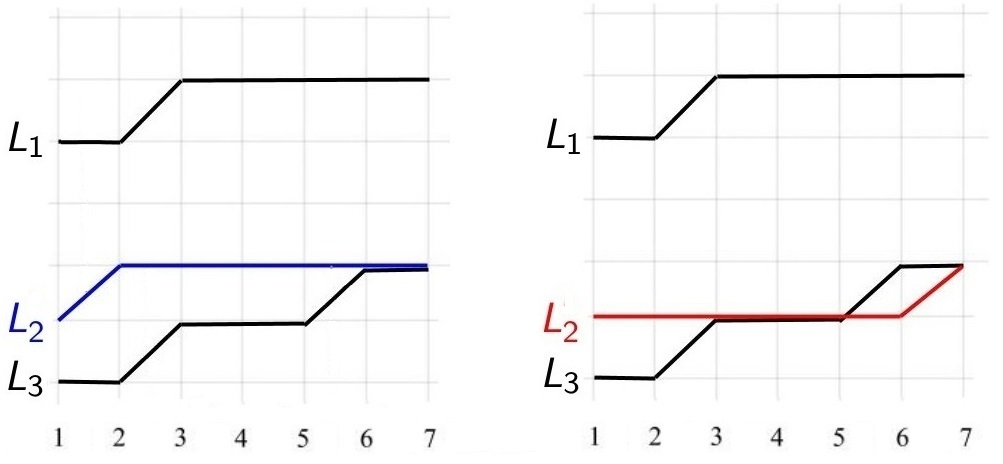
\includegraphics{S3_1.jpg}}
\caption{Two samples of $\{1,2,3\}$-indexed Bernoulli line ensembles with $T_0 = 1$ and $T_1 = 7$. }
\label{S3_1}
\end{figure}
We will often slightly abuse notation and write $\mathfrak{L}: \Sigma \times \llbracket T_0, T_1 \rrbracket \rightarrow \mathbb{Z}$, even though it is not $\mathfrak{L}$ which is such a function, but rather $\mathfrak{L}(\omega)$ for each $\omega \in \Omega$. Furthermore we write $L_i = (\mathfrak{L}(\omega)) (i, \cdot)$ for the index $i \in \Sigma$ path. If $L$ is an up-right path on $\llbracket T_0, T_1 \rrbracket$ and $a, b \in \llbracket T_0, T_1 \rrbracket$ satisfy $a < b$ we let $L\llbracket a, b \rrbracket$ denote the resitrction of $L$ to $\llbracket a,b\rrbracket$. \\

Let $t_i, z_i \in \mathbb{Z}$ for $i = 1,2$ be given such that $t_1 < t_2$ and $0 \leq z_2 - z_1 \leq t_2 - t_1$. We denote by $\Omega(t_1,t_2,z_1,z_2)$ the collection of up-right paths that start from $(t_1,z_1)$ and end at $(t_2,z_2)$, by $\mathbb{P}_{Ber}^{t_1,t_2, z_1, z_2}$ the uniform distribution on $\Omega(t_1,t_2,z_1,z_2)$ and write $\mathbb{E}^{t_1,t_2,z_1,z_2}_{Ber}$ for the expectation with respect to this measure. One thinks of the distribution $\mathbb{P}_{Ber}^{t_1,t_2, z_1, z_2}$ as the law of a simple random walk with i.i.d. Bernoulli increments with parameter $p \in (0,1)$ that starts from $z_1$ at time $t_1$ and is conditioned to end in $z_2$ at time $t_2$ -- this interpretation does not depend on the choice of $p \in (0,1)$. Notice that by our assumptions on the parameters the state space $\Omega(t_1,t_2,z_1,z_2)$ is non-empty.  

Given $k \in \mathbb{N}$, $T_0, T_1 \in \mathbb{Z}$ with $T_0 < T_1$ and $\vec{x}, \vec{y} \in \mathbb{Z}^k$ we let $\mathbb{P}^{T_0,T_1, \vec{x},\vec{y}}_{Ber}$ denote the law of $k$ independent Bernoulli bridges $\{B_i: \llbracket T_0, T_1 \rrbracket  \rightarrow \mathbb{Z} \}_{i = 1}^k$ from $B_i(T_0) = x_i$ to $B_i(T_1) = y_i$. Equivalently, this is just $k$ independent random up-right paths $B_i \in \Omega(T_0,T_1,x_i,y_i)$ for $i = 1, \dots, k$ that are uniformly distributed. This measure is well-defined provided that $\Omega(T_0,T_1,x_i,y_i)$ are non-empty for $i = 1, \dots, k$, which holds if $T_1 - T_0 \geq y_i - x_i \geq 0$ for all $i = 1, \dots, k$. 



The following definition introduces the notion of an $(f,g)$-avoiding Bernoulli line ensemble, which in simple terms is a collection of $k$ independent Bernoulli bridges, conditioned on not-crossing each other and staying above the graph of $g$ and below the graph of $f$ for two functions $f$ and $g$.
\begin{definition}\label{DefAvoidingLawBer}
Let $k \in \mathbb{N}$ and $\mathfrak{W}_k$ denote the set of signatures of length $k$, i.e.
$$\mathfrak{W}_k = \{ \vec{x} = (x_1, \dots, x_k) \in \mathbb{Z}^k: x_1 \geq  x_2 \geq  \cdots \geq  x_k \}.$$
Let $\vec{x}, \vec{y} \in \mathfrak{W}_k$, $T_0, T_1 \in \mathbb{Z}$ with $T_0 < T_1$, and $f: \llbracket T_0, T_1 \rrbracket \rightarrow (-\infty, \infty]$ and $g: \llbracket T_0, T_1 \rrbracket \rightarrow [-\infty, \infty)$ be two functions. 

With the above data we define the {\em $(f,g)$-avoiding Bernoulli line ensemble on the interval $\llbracket T_0, T_1 \rrbracket$ with entrance data $\vec{x}$ and exit data $\vec{y}$} to be the $\Sigma$-indexed Bernoulli line ensemble $\mathfrak{Q}$ with $\Sigma = \llbracket 1, k\rrbracket$ on $\llbracket T_0, T_1 \rrbracket$ and with the law of $\mathfrak{Q}$ equal to $\mathbb{P}^{T_0,T_1, \vec{x},\vec{y}}_{Ber}$ (the law of $k$ independent uniform up-right paths $\{B_i: \llbracket T_0, T_1 \rrbracket \rightarrow \mathbb{R} \}_{i = 1}^k$ from $B_i(T_0) = x_i$ to $B_i(T_1) = y_i$) conditioned on the event 
$$E  = \left\{ f(r) \geq B_1(r) \geq B_2(r) \geq \cdots \geq B_k(r) \geq g(r) \mbox{ for all $r \in \llbracket T_0, T_1 \rrbracket$} \right\}.$$ 
The above definition is well-posed if there exist $B_i \in \Omega(T_0,T_1,x_i,y_i)$ for $i = 1, \dots, k$ that satisfy the conditions in $E$ (i.e. if the set of such up-right paths is not empty). We will denote by $\Omega_{avoid}(T_0, T_1, \vec{x}, \vec{y}, f,g)$ the set of collections of $k$ up-right paths that satisfy the conditions in $E$ and then the distribution on $\mathfrak{Q}$ is simply the uniform measure on $\Omega_{avoid}(T_0, T_1, \vec{x}, \vec{y}, f,g)$. We denote the probability distribution of $\mathfrak{Q}$ as $\mathbb{P}_{avoid, Ber}^{T_0,T_1, \vec{x}, \vec{y}, f, g}$ and write $\mathbb{E}_{avoid, Ber}^{T_0, T_1, \vec{x}, \vec{y}, f, g}$ for the expectation with respect to this measure. 
\end{definition}

It will be useful to formulate simple conditions under which $\Omega_{avoid}(T_0, T_1, \vec{x}, \vec{y}, f,g)$ is non-empty and thus $\mathbb{P}_{avoid, Ber}^{T_0,T_1, \vec{x}, \vec{y}, f, g}$ well-defined. We accomplish this in the following lemma, whose proof is postponed until Section [Appendix].
\begin{lemma}\label{LemmaWD} Suppose that $k \in \mathbb{N}$ and $T_0, T_1 \in \mathbb{Z}$ with $T_0 < T_1$. Suppose further that $\vec{x}, \vec{y} \in \mathfrak{W}_k$ satisfy $T_1 - T_0 \geq y_i - x_i \geq 0$ for $i = 1, \dots, k$. Suppose further that $f : \llbracket T_0, T_1 \rrbracket \rightarrow (-\infty, \infty]$ and $g : \llbracket T_0, T_1 \rrbracket \rightarrow [-\infty, \infty)$ satisfy $f (i+1) = f(i)$ or $f(i+1) = f(i) + 1$, and $g(i+1) = g(i)$ or $g(i+1) = g(i) +1$ for $i = T_0, \dots, T_1 -1$. Finally, suppose that $f(T_0) \geq x_1, f(T_1) \geq y_1$ and $g(T_0) \leq x_k, g(T_1) \leq y_k$. Then the set $\Omega_{avoid}(T_0, T_1, \vec{x}, \vec{y}, f,g)$ from Definition \ref{DefAvoidingLawBer} is non-empty.
\end{lemma}

The following definition introduces the notion of the Schur Gibbs property, which can be thought of a discrete analogue of the partial Brownian Gibbs property the same way that Bernoulli random walks are discrete analogues of Brownian motion. 
\begin{definition}\label{DefSGP}
Fix a set $\Sigma = \llbracket 1, N \rrbracket$ with $N \in \mathbb{N}$ or $N = \infty$ and $T_0, T_1\in \mathbb{Z}$ with $T_0 < T_1$. A $\Sigma$-indexed Bernoulli line ensemble $\mathfrak{L} : \Sigma \times \llbracket T_0, T_1 \rrbracket \rightarrow \mathbb{Z}$ is said to satisfy the {\em Schur Gibbs property} if it is non-crossing, meaning that 
$$ L_j(i) \geq L_{j+1}(i) \mbox{ for all $j = 1, \dots, N-1$ and $i \in \llbracket T_0, T_1 \rrbracket$},$$
and for any finite $K = \{k_1, k_1 + 1, \dots, k_2 \} \subset \llbracket 1, N - 1 \rrbracket$ and $a,b \in \llbracket T_0, T_1 \rrbracket$ with $a < b$ the following holds.  Suppose that $f, g$ are two up-right paths drawn in $\{ (r,z) \in \mathbb{Z}^2 : a \leq r \leq b\}$ and $\vec{x}, \vec{y} \in \mathfrak{W}_{k_2 - k_1 + 1}$ altogether satisfy that $\mathbb{P}(A) > 0$ where $A$ denotes the event
$$A =\{  ({L}_{k_1}(a), \dots, {L}_{k_2}(a)), \vec{y} = ({L}_{k_1}(b), \dots, {L}_{k_2}(b)), L_{k_1-1} \llbracket a,b \rrbracket = f, L_{k_2+1} \llbracket a,b \rrbracket = g \},$$
where if $k_1 = 1$ we adopt the convention $f = \infty = L_0$. Then for any $\{ B_i \in \Omega(a, b, x_i , y_i) \}_{i = 1}^{k_2 - k_1 +1}$ 
\begin{equation}\label{SchurEq}
\mathbb{P}\left( L_{i + k_1-1}\llbracket a,b \rrbracket = B_{i} \mbox{ for $i = 1, \dots, k_2 - k_1 + 1$} \vert  A \right) = \mathbb{P}_{avoid, Ber}^{T_0,T_1, \vec{x}, \vec{y}, f, g} \left( \cap_{i = 1}^k\{ \mathfrak{Q}_i = B_i \} \right).
\end{equation}
\end{definition}
\begin{remark}\label{RemSGB} In simple words, a Bernoulli line ensemble is said to satisfy the Schur Gibbs property if the distribution of any finite number of consecutive paths, conditioned on their end-points and the paths above and below them is simply the uniform measure on all collection of up-right paths that have the same end-points and do not cross each other or the paths above and below them. 
\end{remark}

\begin{remark}\label{RemSGB2} Observe that in Definition \ref{DefSGP} the index $k_2$ is assumed to be less than or equal to $N-1$, so that if $N < \infty$ the $N$-th path is special and is not conditionally uniform. This is what makes Definition \ref{DefSGP} a discrete analogue of the partial Brownian Gibbs property rather than the usual Brownian Gibbs property. Similarly to the partial Brownian Gibbs propert, see Remark \ref{BGPDeg}, if $N = 1$ then the conditions in Definition \ref{DefSGP} become void. I.e., any Bernoulli line ensemble with one line satisfies the Schur Gibbs property. Also we mention that the well-posedness of $\mathbb{P}_{avoid, Ber}^{T_0,T_1, \vec{x}, \vec{y}, f, g}$ in (\ref{SchurEq}) is a consequence of Lemma \ref{LemmaWD} and our assumption that $\mathbb{P}(A) > 0$.
\end{remark}

\begin{remark} In \cite{CD} the authors studied a generalization of the Gibbs property in Definition \ref{DefSGP} depending on a parameter $t \in (0,1)$, which was called the {\em Hall-Littlewood Gibbs property} due to its connection to Hall-Littlewood polynomials \cite{Mac}. The property in Definition \ref{DefSGP} is the $t \rightarrow 0$ limit of the Hall-Littlewood Gibbs property. Since under this $t \rightarrow 0$ limit Hall-Littlewood polynomials degenerate to Schur polynomials we have decided to call the Gibbs property in Definition \ref{DefSGP} the Schur Gibbs property.
\end{remark}
\begin{remark} \label{restrict}  An immediate consequence of Definition \ref{DefSGP} is that if $M \leq N$, we have that the induced law on $\{L_i\}_{i = 1}^M$ also satisfies the Schur Gibbs property as an $\{1,\dots,M\}$-indexed Bernoulli line ensemble on $\llbracket T_0, T_1 \rrbracket$.
\end{remark}

We end this section with the following definition of the term acceptance probability. 
\begin{definition}\label{DefAP} Assume the same notation as in Definition \ref{DefAvoidingLawBer} and suppose that $ T_1 - T_0 \geq y_i -x_i \geq 0$ for $i =1, \dots, k$. We define the {\em acceptance probability } $Z(  T_0, T_1, \vec{x}, \vec{y}, f, g)$ to be the ratio
\begin{equation}\label{EqAP}
Z(  T_0, T_1, \vec{x}, \vec{y}, f, g) = \frac{|\Omega_{avoid}(T_0, T_1, \vec{x}, \vec{y}, f,g)|}{\prod_{i = 1}^k |\Omega(T_0, T_1, x_i, y_i)|}.
\end{equation}
\end{definition}
\begin{remark}\label{RemAP} The quantity $Z(  T_0, T_1, \vec{x}, \vec{y}, f, g)$ is precisely the probability that if $B_i$ are sampled uniformly from $\Omega(T_0, T_1, x_i, y_i)$ for $i =1 , \dots, k$ then the $B_i$ satisfy the condition
$$ E=  \left\{ f(r) \geq B_1(r) \geq B_2(r) \geq \cdots \geq B_k(r) \geq g(r) \mbox{ for all $r \in \llbracket T_0, T_1 \rrbracket$} \right\}.$$
 Let us explain briefly why we call this quantity an acceptance probability. One way to sample $\mathbb{P}_{avoid, Ber}^{T_0,T_1, \vec{x}, \vec{y}, f, g}$ is as follows. Start by sampling a sequence of i.i.d. up-right paths $B^N_i$ uniformly from $\Omega(T_0, T_1, x_i, y_i)$ for $i =1 , \dots, k$ and $N \in \mathbb{N}$. For each $n$ check if $B^n_1, \dots, B^n_k$ satisfy the condition $E$ and let $M$ denote the smallest index that accomplishes this. If $\Omega_{avoid}(T_0, T_1, \vec{x}, \vec{y}, f,g)$ is non-empty then $M$ is geometrically distributed with parameter $Z(  T_0, T_1, \vec{x}, \vec{y}, f, g)$, and in particular $M$ is finite almost surely and $\{B^M_i\}_{i =1}^k$ has distribution $\mathbb{P}_{avoid, Ber}^{T_0,T_1, \vec{x}, \vec{y}, f, g}$. In this sampling procedure we construct a sequence of candidates $\{B^N_i\}_{i =1}^k$ for $N \in \mathbb{N}$ and reject those that fail to satisfy condition $E$, the first candidate that satisfies it is accepted and has law $\mathbb{P}_{avoid, Ber}^{T_0,T_1, \vec{x}, \vec{y}, f, g}$ and the probability that a candidate is accepted is precisely $Z(  T_0, T_1, \vec{x}, \vec{y}, f, g)$, which is why we call it an acceptance probability.
\end{remark}



%-------------------------------------------------------------------------------------------------------------------------------------------------------------------------------------------------
% Section 2.3
%
%-------------------------------------------------------------------------------------------------------------------------------------------------------------------------------------------------
\subsection{Main result}\label{Section2.3} In this section we present the main result of the paper. We start with the following technical definition.
\begin{definition}\label{Def1} Fix $k \in \mathbb{N}$, $\alpha, \lambda > 0$ and $p \in (0,1)$. Suppose we are given a sequence $\{ T_N \}_{N = 1}^\infty$ with $T_N \in \mathbb{N}$ and that $\{\mathfrak{L}^N\}_{N = 1}^\infty$, $\mathfrak{L}^N = (L^N_1, L^N_2, \dots, L^N_k)$ is a sequence of $\llbracket 1, k \rrbracket$-indexed Bernoulli line ensembles on $ \llbracket -T_N, T_N \rrbracket$. We call the sequence $(\alpha,p,\lambda)$-{\em good} if 
\begin{itemize}
\item for each $N \in \mathbb{N}$ we  have that $\mathfrak{L}^N$ satisfies the Schur Gibbs property of Definition \ref{DefSGP};  
\item there is a function $\psi: \mathbb{N} \rightarrow (0, \infty)$ such that $\lim_{N \rightarrow \infty} \psi(N) = \infty$ and for each $N \in \mathbb{N}$ we have that $ T_N > \psi(N)N^{\alpha}$;
\item  there is a function $\phi: (0, \infty) \rightarrow (0,\infty)$ such that for any $\epsilon > 0$ we have 
\begin{equation}\label{globalParabola}
 \sup_{n \in \mathbb{Z}} \limsup_{N \rightarrow \infty} \mathbb{P} \left( \left|N^{-\alpha/2}(L_1^N(n N^{\alpha}) - p n N^{\alpha} + \lambda n^2 N^{\alpha/2}) \right| \geq \phi(\epsilon) \right) \leq \epsilon.
\end{equation}
\end{itemize}
\end{definition}
\begin{remark} Let us elaborate on the meaning of Definition \ref{Def1}. In order for a sequence of $\mathfrak{L}^N $ of $\llbracket 1, k \rrbracket$-indexed Bernoulli line ensembles on $ \llbracket -T_N, T_N \rrbracket$ to be $(\alpha,p,\lambda)$-{\em good} we want several conditions to be satisfied. Firstly, we want for each $N$ the Bernoulli line ensemble $\mathfrak{L}^N$ to satisfy the Schur Gibbs property. The second condition is that while the interval of definition of $\mathfrak{L}^N$ is finite for each $N$ and given by $\llbracket -T_N, T_N \rrbracket$, we want this interval to grow at least with speed $N^{\alpha}$. This property is quantified by the function $\psi$, which can be essentially thought of as an arbitrary unbounded increasing function on $\mathbb{N}$. The third condition is that we want for each $n \in \mathbb{Z}$ the sequence of random variables $N^{-\alpha/2}(L_1^N(n N^{\alpha}) - p n N^{\alpha})$ to be tight but moreover we want globally these random variables to look like the parabola $-\lambda n^2$. This statement is reflected in (\ref{globalParabola}), which provides a certain uniform tightness of the random variables $N^{-\alpha/2}(L_1^N(n N^{\alpha}) - p n N^{\alpha} + \lambda n^2 N^{\alpha/2}) $. A particular case when (\ref{globalParabola}) is satisfied is for example if we know that  for each $n \in \mathbb{Z}$ the random variables $N^{-\alpha/2}(L_1^N(n N^{\alpha}) - p n N^{\alpha} + \lambda n^2 N^{\alpha/2})$ converge to the same random variable $X$. In the applications that we have in mind these random variables would converge to the $1$-point marginals of the Airy$_2$ process that are all given by the same Tracy-Widom distribution (since the Airy$_2$ process is stationary). Equation (\ref{globalParabola}) is a significant relaxation of the requirement that $N^{-\alpha/2}(L_1^N(n N^{\alpha}) - p n N^{\alpha} + \lambda n^2 N^{\alpha/2})$ all converge weakly to the Tracy-Widom distribution -- the convergence requirement is replaced with a mild but uniform control of all subsequential limits.
\end{remark}

The main result of the paper is as follows.
\begin{theorem}\label{PropTightGood}
Fix $k \in \mathbb{N}$ with $k \geq 2$, $\alpha, \lambda > 0$ and $p \in (0,1)$ and let $\mathfrak{L}^N = (L^N_1, L^N_2, \dots, L^N_k)$ be an $(\alpha, p, \lambda)$-good sequence of $\llbracket 1, k \rrbracket$-indexed Bernoulli line ensembles.  Set
$$f^N_i(s) =  N^{-\alpha/2}(L^N_i(sN^{\alpha}) - p s N^{\alpha} + \lambda s^2 N^{\alpha/2}), \mbox{ for $s\in [-\psi(N) ,\psi(N)]$ and $i = 1,\dots, k -1$,}$$
and extend $f^N_i$ to $\mathbb{R}$ by setting for $i = 1, \dots, k - 1$
$$f^N_i(s) = f^N_i(-\psi(N)) \mbox{ for $s \leq -\psi(N)$ and } f^N_i(s) = f_N(\psi(N)) \mbox{ for $s \geq \psi(N)$}.$$
Let $\mathbb{P}_N$ denote the law of $\{f^N_i\}_{i = 1}^{k-1}$ as a $\llbracket 1, k-1 \rrbracket$-indexed line ensemble (i.e. as a random variable in $(C( \llbracket 1, k -1 \rrbracket \times \mathbb{R}), \mathcal{C})$). Then the sequence $\mathbb{P}_N$ is tight.
\end{theorem}

Roughly, Theorem \ref{PropTightGood} states that if you have a sequence of $\llbracket 1, k \rrbracket$-indexed Bernoulli line ensembles that satisfy the Schur Gibbs property and the top paths of these ensembles under some shift and scaling have tight one-point marginals with a non-trivial parabolic shift, then  under the same shift and scaling the top $k-1$ paths of the line ensemble will be tight. The extension of $f^N_i$ to $\mathbb{R}$ is completely arbitrary and irrelevant for the validity of Theorem \ref{PropTightGood} since the topology on $C( \llbracket 1, k -1 \rrbracket \times \mathbb{R})$ is that of uniform convergence over compacts. Consequently, only the behavior of these functions on compact intervals matters in Theorem \ref{PropTightGood} and not what these functions do near infinity, which is where the modification happens as $\lim_{N \rightarrow \infty} \psi(N) = \infty$  by assumption. The only reason we perform the extension is to embed all Bernoulli line ensembles into the same space $(C( \llbracket 1, k -1 \rrbracket \times \mathbb{R}), \mathcal{C})$.

 We mention that the $k$-th up-right path in the sequence of Bernoulli line ensembles is special and Theorem \ref{PropTightGood} provides no tightness result for it. The reason for this stems from the Schur Gibbs property, see Definition \ref{DefSGP}, which assumes less information for the $k$-th path. In practice, one either has an infinite Bernoulli line ensemble for each $N$ or one has a Bernoulli line ensemble with finite number of paths, which increase with $N$ to infinity. In either of these settings one can use Theorem \ref{PropTightGood} to prove teightness of the full line ensemble - we will have more to say about this in Section [Applications].

The proof of Theorem \ref{PropTightGood} is presented in Section \ref{Section4}. In the next section we derive various properties for Bernoulli line ensembles.








%-------------------------------------------------------------------------------------------------------------------------------------------------------------------------------------------------
% Section 3
%
%-------------------------------------------------------------------------------------------------------------------------------------------------------------------------------------------------
\section{Properties of Bernoulli line ensembles}\label{Section3} In this section we derive several results for Bernoulli line ensembles, which will be used in the proof of Theorem \ref{PropTightGood} in Section \ref{Section4}.


%-------------------------------------------------------------------------------------------------------------------------------------------------------------------------------------------------
% Section 3.1
%
%-------------------------------------------------------------------------------------------------------------------------------------------------------------------------------------------------
\subsection{Monotone coupling lemmas}\label{Section3.1}
 In this section we formulate two lemmas that provide couplings of two Bernoulli line ensembles of non-intersecting Bernoulli bridges on the same interval, which depend monotonically on their boundary data. Schematic depictions of the couplings are provided in Figure \ref{fig:MCL}. We postpone the proof of these lemmas until Section \ref{AppendixA}. 
\begin{figure}[ht]
  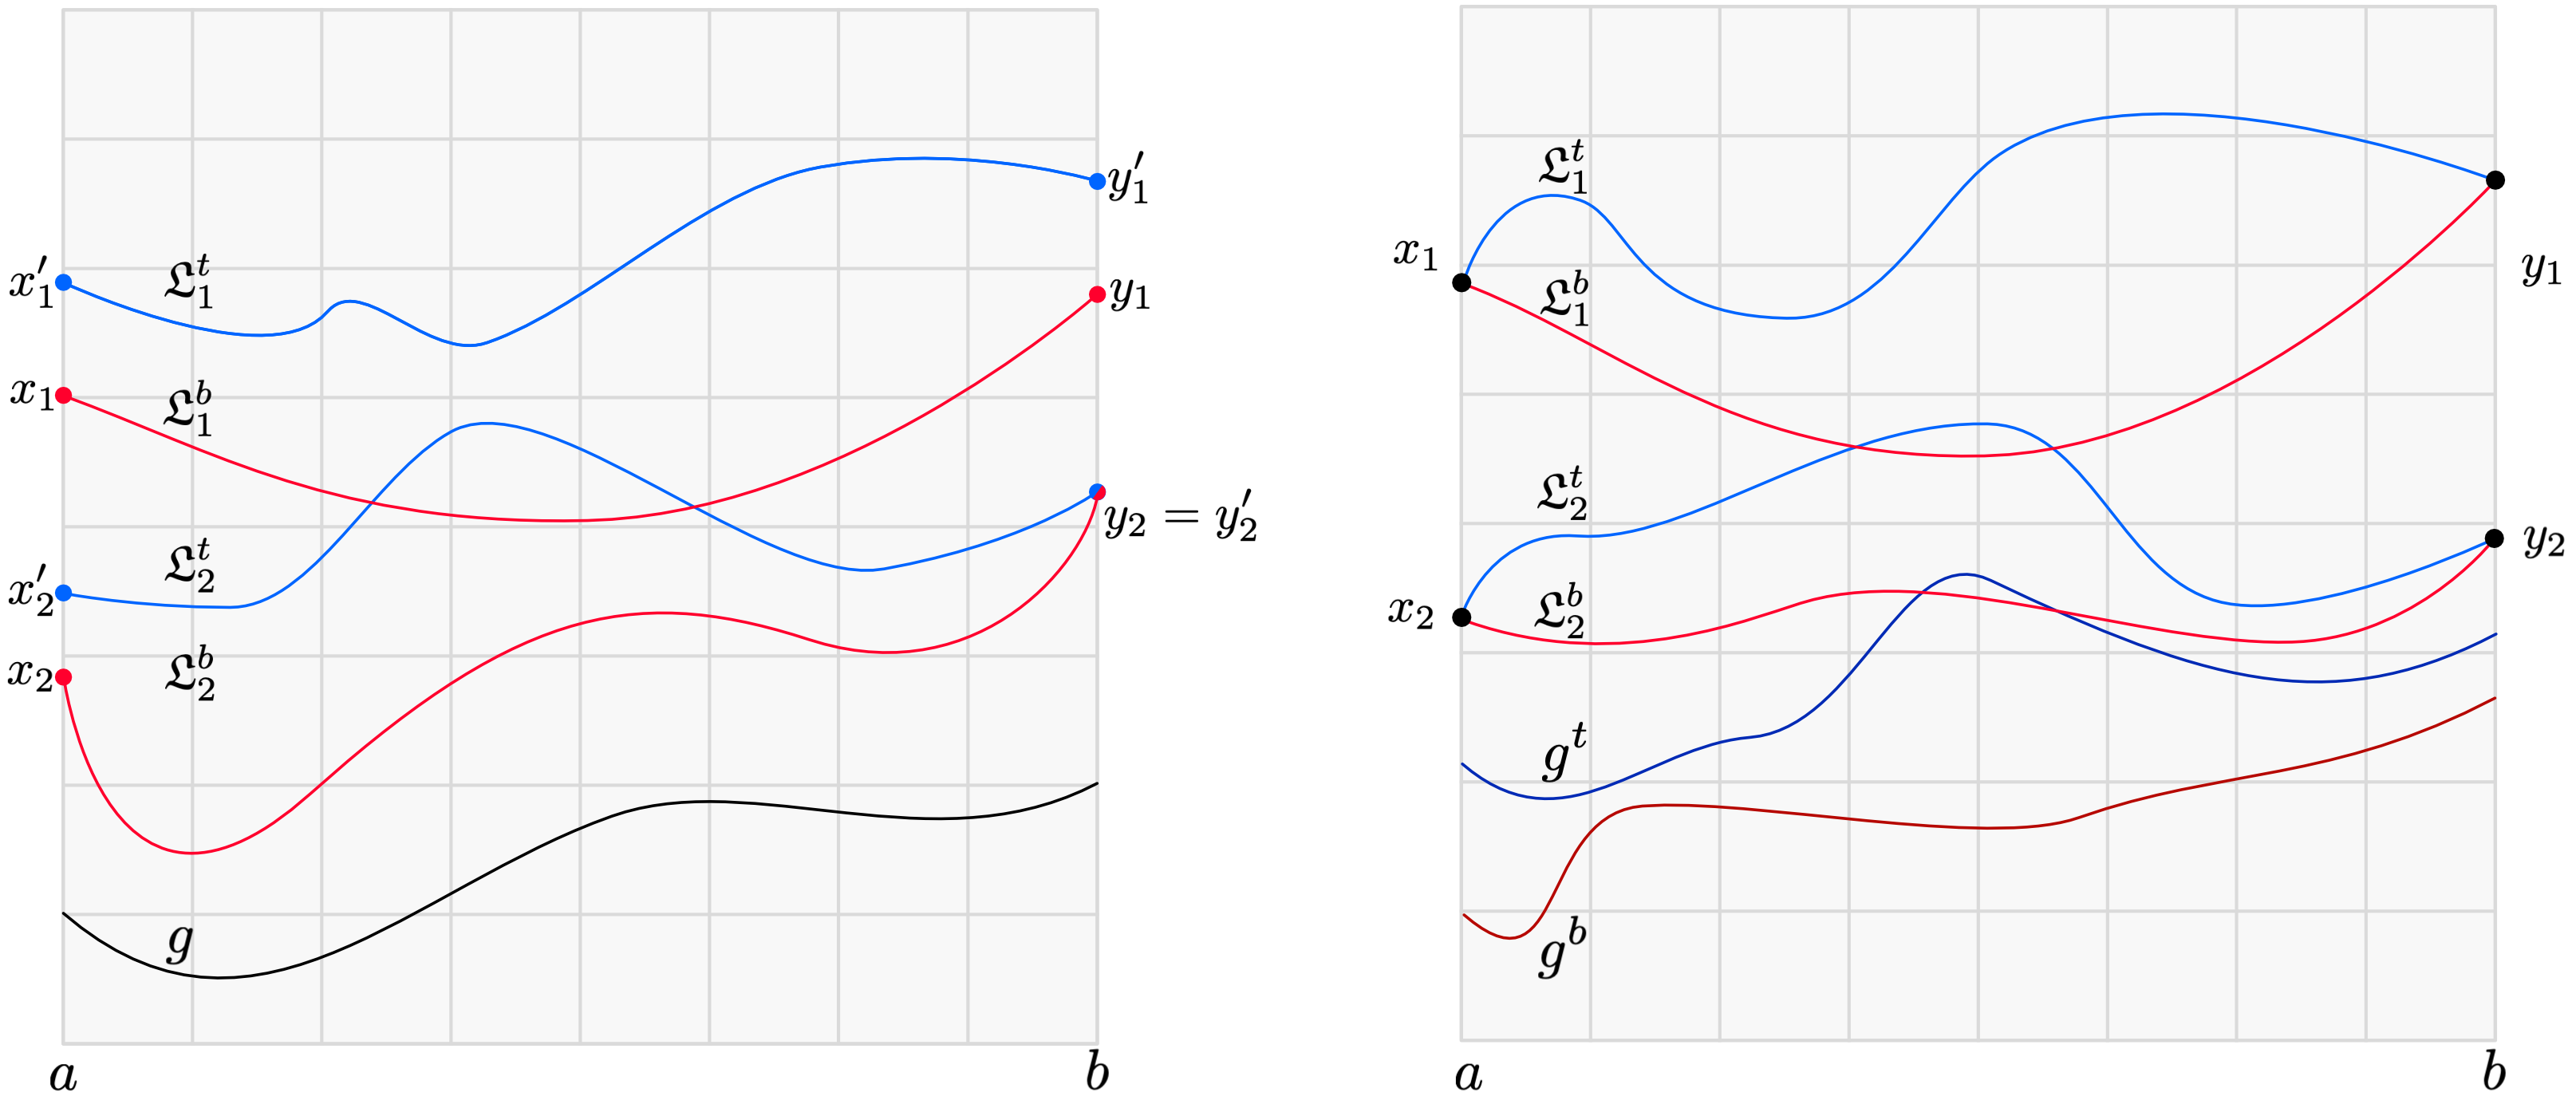
\includegraphics[width=1.02\textwidth]{graphics/MonotoneCoupling.png}
  \caption{Two diagrammatic depictions of the monotone coupling Lemma \ref{MCLxy} (left part) and Lemma \ref{MCLfg} (right part). Red depicts the lower line ensemble and accompanying entry data, exit data, and bottom bounding curve, while blue depicts that of the higher ensemble.}
  \label{fig:MCL}
\end{figure}

\begin{lemma}\label{MCLxy} Assume the same notation as in Definition \ref{DefAvoidingLawBer}. Fix $k \in \mathbb{N}$, $T_0, T_1 \in \mathbb{Z}$ with $T_0 < T_1$, a function $g: \llbracket T_0, T_1 \rrbracket  \rightarrow [-\infty, \infty)$ as well as $\vec{x}, \vec{y}, \vec{x}\,', \vec{y}\,' \in \mathfrak{W}_k$. Assume that $\Omega_{avoid}(T_0, T_1, \vec{x}, \vec{y}, \infty,g)$ and $\Omega_{avoid}(T_0, T_1, \vec{x}', \vec{y}', \infty,g)$ are both non-empty. Then there exists a probability space $(\Omega, \mathcal{F}, \mathbb{P})$, which supports two $\llbracket 1, k \rrbracket$-indexed Bernoulli line ensembles $\mathfrak{L}^t$ and $\mathfrak{L}^b$ on $\llbracket T_0, T_1 \rrbracket$ such that the law of $\mathfrak{L}^{t}$ {\big (}resp. $\mathfrak{L}^b${\big )} under $\mathbb{P}$ is given by $\mathbb{P}_{avoid, Ber}^{T_0, T_1, \vec{x}\,', \vec{y}\,', \infty, g}$ {\big (}resp. $\mathbb{P}_{avoid, Ber}^{T_0, T_1, \vec{x}, \vec{y}, \infty, g}${\big )} and such that $\mathbb{P}$-almost surely we have $\mathfrak{L}_i^t(r) \geq \mathfrak{L}^b_i(r)$ for all $i = 1,\dots, k$ and $r \in \llbracket T_0, T_1 \rrbracket$.
\end{lemma}

\begin{lemma}\label{MCLfg} Assume the same notation as in Definition \ref{DefAvoidingLawBer}. Fix $k \in \mathbb{N}$,  $T_0, T_1 \in \mathbb{Z}$ with $T_0 < T_1$, two functions $g^t, g^b: \llbracket T_0, T_1 \rrbracket \rightarrow [-\infty,\infty)$ and $\vec{x}, \vec{y} \in \mathfrak{W}_k$. We assume that $g^t(r) \geq g^b(r)$ for all $r \in \llbracket T_0, T_1 \rrbracket$ and that $\Omega_{avoid}(T_0, T_1, \vec{x}, \vec{y}, \infty,g^t)$ and $\Omega_{avoid}(T_0, T_1, \vec{x}, \vec{y}, \infty,g^b)$ are both non-empty. Then there exists a probability space $(\Omega, \mathcal{F}, \mathbb{P})$, which supports two $\llbracket 1, k \rrbracket$-indexed Bernoulli line ensembles $\mathfrak{L}^t$ and $\mathfrak{L}^b$ on $\llbracket T_0, T_1 \rrbracket$ such that the law of $\mathfrak{L}^{t}$ {\big (}resp. $\mathfrak{L}^b${\big )} under $\mathbb{P}$ is given by $\mathbb{P}_{avoid, Ber}^{T_0, T_1, \vec{x}, \vec{y}, \infty, g^t}$ {\big (}resp. $\mathbb{P}_{avoid, Ber}^{T_0,T_1, \vec{x}, \vec{y}, \infty, g^b}${\big )} and such that $\mathbb{P}$-almost surely we have $\mathfrak{L}_i^t(r) \geq \mathfrak{L}^b_i(r)$ for all $i = 1,\dots, k$ and $r \in \llbracket T_0, T_1 \rrbracket$.
\end{lemma}

In plain words, Lemma \ref{MCLxy} states that one can couple two Bernoulli line ensembles $\mathfrak{L}^{t}$ and $\mathfrak{L}^{b}$ of non-intersecting Bernoulli bridges, bounded from below by the same function $g$, in such a way that if all boundary values of $\mathfrak{L}^{t}$ are above the respective boundary values of $\mathfrak{L}^{b}$, then all up-right paths of $\mathfrak{L}^{t}$ are almost surely above the respective up-right paths of $\mathfrak{L}^{b}$. See the left part of Figure \ref{fig:MCL}. Lemma \ref{MCLfg}, states that one can couple two Bernoulli line ensembles $\mathfrak{L}^{t}$ and $\mathfrak{L}^{b}$ that have the same boundary values, but the lower bound $g^t$ of $\mathfrak{L}^{t}$ is above the lower bound $g^b$ of $\mathfrak{L}^{b}$, in such a way that all up-right paths of $\mathfrak{L}^{t}$ are almost surely above the respective up-right paths of $\mathfrak{L}^{b}$. See the right part of Figure \ref{fig:MCL}.


%-------------------------------------------------------------------------------------------------------------------------------------------------------------------------------------------------
% Section 3.2
%
%-------------------------------------------------------------------------------------------------------------------------------------------------------------------------------------------------
\subsection{Properties of Bernoulli bridges}\label{Section3.2} In this section we derive several results about Bernoulli bridges, which are random up-right paths that have law $\mathbb{P}_{Ber}^{T_0, T_1, x,y}$ as in Section \ref{Section2.2}. Our results will rely on the two monotonicity Lemmas \ref{MCLxy} and \ref{MCLfg} as well as a strong coupling between Bernoulli bridges and Brownian bridges from \cite{CD} -- recalled here as Theorem \ref{KMT}.

If $W_t$ denotes a standard one-dimensional Brownian motion and $\sigma > 0$, then the process
$$B^{\sigma}_t = \sigma (W_t - t W_1), \hspace{5mm} 0 \leq t \leq 1,$$
is called a {\em Brownian bridge (conditioned on $B_0 = 0, B_1 = 0$) with variance $\sigma^2$.} We note that $B^\sigma$ is the unique a.s. continuous Gaussian process on $[0,1]$ with $B_0 = B_1  = 0$, $\ex[B^\sigma_t] = 0$, and
\begin{equation}\label{BBcovar}
\ex[B^\sigma_r B^\sigma_s] = \sigma^2(r\wedge s - rs - sr + sr) = \sigma^2 (r\wedge s - rs).
\end{equation}  
With the above notation we state the strong coupling result we use.
\begin{theorem}\label{KMT}
Let $p \in (0,1)$. There exist constants $0 < C, a, \alpha < \infty$ (depending on $p$) such that for every positive integer $n$, there is a probability space on which are defined a Brownian bridge $B^\sigma$ with variance $\sigma^2 = p(1-p)$ and a family of random paths $\ell^{(n,z)} \in \Omega(0,n, 0, z)$ for $z = 0,\dots,n$ such that $\ell^{(n,z)}$ has law $\mathbb{P}^{0,n,0,z}_{Ber}$ and
\begin{equation}\label{KMTeq}
\mathbb{E}\left[ e^{a \Delta(n,z)} \right] \leq C e^{\alpha (\log n)^2}e^{|z- p n|^2/n}, \mbox{ where $\Delta(n,z):=  \sup_{0 \leq t \leq n} \left| \sqrt{n} B^\sigma_{t/n} + \frac{t}{n}z - \ell^{(n,z)}(t) \right|.$}
\end{equation}
\end{theorem}
\begin{remark} When $p = 1/2$ the above theorem follows (after a trivial affine shift) from \cite[Theorem 6.3]{LF} and the general $p \in (0,1)$ case was done in \cite[Theorem 4.5]{CD}. We mention that a significant generalization of Theorem \ref{KMT} for general random walk bridges has recently been proved in \cite[Theorem 2.3]{DW19}.
\end{remark}

We will use the following simple corollary of Theorem \ref{KMT} in the following to compare Bernoulli bridges with Brownian bridges. We use the same notation as in the theorem.

\begin{corollary}\label{Cheb}
	Fix $p\in (0,1)$, $\beta > 0$, and $A>0$. Suppose $|z-pn| \leq K\sqrt{n}$ for a constant $K>0$. Then for any $\epsilon > 0$, there exists $N$ large enough depending on $p,\epsilon,A,K$ so that for $n\geq N$,
	\[
	\mathbb{P}\Big(\Delta(n,z) \geq An^\beta\Big) < \epsilon.
	\]
\end{corollary}

\begin{proof}
	Applying Chebyshev's inequality and \eqref{KMTeq} gives
	\begin{align*}
	\mathbb{P}\Big(\Delta(n,z) \geq An^\beta\Big) &\leq e^{-An^\beta}\ex\Big[e^{a\Delta(n,z)}\Big] \leq C\exp\Big[-An^\beta + \alpha(\log n)^2 + \frac{|z-pn|^2}{n}\Big]\\
	&\leq C\exp\Big[-An^\beta + \alpha(\log n)^2 + K\Big].
	\end{align*}
	The conclusion is now immediate.
\end{proof}

We also state the following result regarding the distribution of the maximum of a Brownian bridge, which follows from a formula in \cite[Chapter 4]{KS}.

\begin{lemma}\label{BBmax}
	Fix $p\in (0,1)$, and let $B^\sigma$ be a Brownian bridge of variance $\sigma^2 = p(1-p)$ on $[0,1]$. Then for any $C,T> 0$ we have
	\[
	\mathbb{P}\Big(\max_{s\in[0,T]} B^\sigma_{s/T} \geq C\Big) = \exp\left( - \frac{2C^2}{p(1-p)}\right) \quad \mathrm{and} \quad \mathbb{P}\Big(\max_{s\in[0,T]} \big|B^\sigma_{s/T}\big| \geq C\Big) \leq 2\exp\left( - \frac{2C^2}{p(1-p)}\right).
	\]
\end{lemma}

\begin{proof}
	Let $B^1$ be a Brownian bridge with variance 1 on $[0,1]$. Then $B^\sigma_t$ has the same distribution as $\sigma B^1_t$. Hence
	\begin{align*}
	\mathbb{P}\Big( \max_{s\in[0,T]} B^\sigma_{s/T} \geq C \Big) &= \mathbb{P}\Big( \max_{t\in[0,1]} B^1_t \geq C/\sigma \Big) = e^{-2(C/\sigma)^2} = e^{-2C^2/p(1-p)}.
	\end{align*}
	The second equality follows from \cite[Chapter 4, (3.40)]{KS}. We now observe that since $B^\sigma_t$ has mean 0, $B^\sigma_t$ and $-B^\sigma_t$ have the same distribution. Hence by the equality just proven,
	\begin{align*}
	\mathbb{P}\Big( \max_{s\in[0,T]} \big| B^\sigma_{s/T}\big| \geq C \Big) &\leq \mathbb{P}\Big( \max_{s\in[0,T]}  B^\sigma_{s/T} \geq C \Big) + \mathbb{P}\Big( \max_{s\in[0,T]}  \big(-B^\sigma_{s/T}\big) \geq C \Big)\\
	&= 2\,\mathbb{P}\Big( \max_{s\in[0,T]}  B^\sigma_{s/T} \geq C \Big) = 2e^{-2C^2/p(1-p)}.
	\end{align*}
\end{proof}

We state one more lemma about Brownian bridges, which allows us to decompose a bridge on $[0,1]$ into two independent bridges with Gaussian affine shifts meeting at a point in $(0,1)$.

\begin{lemma}\label{2bridges}
	Fix $p\in (0,1)$, $T>0$, $t\in(0,T)$, and let $B^\sigma$ be a Brownian bridge of variance $\sigma^2 = p(1-p)$ on $[0,1]$. Let $\xi$ be a Gaussian random variable with mean 0 and variance
	\[
	\ex[\xi^2] = \sigma^2\frac{t}{T}\left(1-\frac{t}{T}\right).
	\]
	Let $B^1,B^2$ be two independent Brownian bridges on $[0,1]$ with variances $\sigma^2 t/T$ and $\sigma^2(T-t)/T$ respectively, also independent from $B^\sigma$. Define the process
	\[
	\tilde{B}_{s/T} = \begin{dcases}
	\frac{s}{t}\,\xi + B^1\Big(\frac{s}{t}\Big), & s\leq t,\\
	\frac{T-s}{T-t}\,\xi + B^2\Big(\frac{s-t}{T-t}\Big), & s\geq t,
	\end{dcases}
	\]
	for $s\in [0,T]$. Then $\tilde{B}$ is a Brownian bridge with variance $\sigma$.
\end{lemma}

\begin{proof}
	It is clear that the process $\tilde{B}$ is a.s. continuous, and each $\tilde{B}_s$ is Gaussian with mean 0 since it is a linear combination of centered Gaussians. By \ref{BBcovar}, it suffices to verify that if $0\leq r\leq s\leq T$, then
	\begin{equation}\label{covar}
	\ex[\tilde{B}_{r/T}\tilde{B}_{s/T}] = \sigma^2 \frac{r}{T}\Big(1-\frac{s}{T}\Big).
	\end{equation}
	First assume $s\leq t$ Using the fact that $\xi$ and $B^1_\cdot$ are independent with mean 0, we find
	\begin{align*}
	\ex[\tilde{B}_{r/T}\tilde{B}_{s/T}] &= \frac{rs}{t^2}\cdot\sigma^2\frac{t}{T}\Big(1-\frac{t}{T}\Big) + \sigma^2\frac{t}{T}\cdot\frac{r}{t}\Big(1-\frac{s}{t}\Big)\\
	&= \sigma^2\frac{r}{T}\Big(\frac{s}{t} - \frac{s}{T} + 1 - \frac{s}{t}\Big) = \sigma^2\frac{r}{T}\Big(1-\frac{s}{T}\Big).
	\end{align*}
	If $r\geq t$, we compute
	\begin{align*}
	\ex[\tilde{B}_{r/T}\tilde{B}_{s/T}] &= \frac{(T-r)(T-s)}{(T-t)^2}\cdot\sigma^2\frac{t}{T}\Big( 1 - \frac{t}{T}\Big) + \sigma^2\frac{T-t}{T}\cdot\frac{r-t}{T-t}\Big( 1 - \frac{s-t}{T-t}\Big)\\
	&= \frac{\sigma^2(T-s)}{T(T-t)}\Big(\frac{t(T-r)}{T} + r-t\Big) = \frac{\sigma^2(T-s)}{T(T-t)}\cdot\frac{r(T-t)}{T} = \sigma^2\frac{r}{T}\Big(1-\frac{s}{T}\Big).
	\end{align*}
	If $r < t < s$, then since $\xi$, $B^1_\cdot$, and $B^2_\cdot$ are all independent, we have
	\[
	\ex[\tilde{B}_{r/T}\tilde{B}_{s/T}] = \frac{r}{t}\cdot\frac{T-s}{T-t}\cdot\sigma^2\frac{t(T-t)}{T^2} = \sigma^2\frac{r(T-s)}{T^2} = \sigma^2\frac{r}{T}\Big(1-\frac{s}{T}\Big).
	\]
	This proves \eqref{covar} in all cases.
\end{proof}

Below we list six lemmas about Bernoulli bridges. We provide a brief informal explanation of what each result says after it is stated. All six lemmas are proved in a similar fashion. For the first four lemmas one observes that the event, whose probability is being estimated, is monotone in $\ell$. This allows by Lemmas \ref{MCLxy} and \ref{MCLfg} to replace $x,y$ in the statements of the lemmas with the extreme values of the ranges specified in each. Once the choice of $x$ and $y$ is fixed one can use our strong coupling results, Theorem \ref{KMT} and Corollary \ref{Cheb}, to reduce each of the lemmas to an analogous one involving a Brownian bridge with some prescribed variance. The latter statements are then easily confirmed as one has exact formulas for Brownian bridges, such as Lemma \ref{BBmax}.\\

\begin{lemma}\label{LemmaHalfS4} Fix $p \in (0,1)$, $T \in \mathbb{N}$ and $x, y\in \mathbb{Z}$ such that $T \geq y-x \geq 0$, and suppose that $\ell$ has distribution $\mathbb{P}^{0,T,x,y}_{Ber}$. Let $M_1, M_2 \in \mathbb{R}$ be given. Then we can find $W_0 = W_0(p,M_2 - M_1) \in \mathbb{N}$ such that for $T \geq W_0$, $x \geq M_1 T^{1/2}$, $y \geq pT + M_2 T^{1/2}$ and $s \in [0,T]$ we have
\begin{equation}\label{halfEq1S4}
\mathbb{P}^{0,T,x,y}_{Ber}\Big( \ell(s)  \geq \frac{T-s}{T} \cdot M_1 T^{1/2} + \frac{s}{T} \cdot \big(p T + M_2 T^{1/2}\big) - T^{1/4} \Big) \geq \frac{1}{3}.
\end{equation}
\end{lemma}
\begin{remark}
If $M_1, M_2 = 0$ then Lemma \ref{LemmaHalfS4} states that if a Bernoulli bridge $\ell$ is started from $(0,x)$ and terminates at $(T,y)$, which are above the straight line of slope $p$, then at any given time $s \in [0,T]$ the probability that $\ell(s)$ goes a modest distance below the straight line of slope $p$ is upper bounded by $ 2/3$.
\end{remark}
\begin{proof}
	Define $A = \lfloor M_1T^{1/2}\rfloor$ and $B = \lfloor pT + M_2 T^{1/2}\rfloor$. Then since $A\leq x$ and $B\leq y$, it follows from Lemma 3.1 that there is a probability space with measure $\mathbb{P}_0$ supporting random variables $L_1$ and $L_2$, whose laws under $\mathbb{P}_0$ are $\mathbb{P}^{0,T,A,B}_{Ber}$ and $\mathbb{P}^{0,T,x,y}_{Ber}$ respectively, and $\mathbb{P}_0$-a.s. we have $L_1\leq L_2$. Thus
	\begin{align*}
	&\mathbb{P}^{0,T,x,y}_{Ber}\Big( \ell(s)  \geq \frac{T-s}{T} \cdot M_1 T^{1/2} + \frac{s}{T} \cdot \big(p T + M_2 T^{1/2}\big) - T^{1/4} \Big)\\
	= \; & \mathbb{P}_0\Big( L_2(s)  \geq \frac{T-s}{T} \cdot M_1 T^{1/2} + \frac{s}{T} \cdot \big(p T + M_2 T^{1/2}\big) - T^{1/4} \Big)\\
	\geq \; & \mathbb{P}_0\Big( L_1(s)  \geq \frac{T-s}{T} \cdot M_1 T^{1/2} + \frac{s}{T} \cdot \big(p T + M_2 T^{1/2}\big) - T^{1/4} \Big)\\
	= \; & \mathbb{P}^{0,T,A,B}_{Ber}\Big( \ell(s)  \geq \frac{T-s}{T} \cdot M_1 T^{1/2} + \frac{s}{T} \cdot \big(p T + M_2 T^{1/2}\big) - T^{1/4} \Big).
	\end{align*}
	Since upright paths on $\llbracket 0,T\rrbracket \times \llbracket A,B\rrbracket$ are equivalent to upright paths on $\llbracket 0,T\rrbracket \times \llbracket 0, B-A\rrbracket$ shifted vertically by $A$, the last line is equal to
	\[
	\mathbb{P}^{0,T,0,B-A}_{Ber}\Big( \ell(s) + A  \geq \frac{T-s}{T} \cdot M_1 T^{1/2} + \frac{s}{T} \cdot \big(p T + M_2 T^{1/2}\big) - T^{1/4} \Big).
	\]
	Now we consider the coupling provided by Theorem \ref{KMT}. We have another probability space $(\Omega,\mathcal{F},\mathbb{P})$ supporting a random variable $\ell^{(T,B-A)}$ whose law under $\mathbb{P}$ is $\mathbb{P}^{0,T,0,B-A}_{Ber}$, and a Brownian bridge $B^\sigma$. Then 
	\begin{align*}
	&\mathbb{P}^{0,T,0,B-A}_{Ber}\Big( \ell(s) + A  \geq \frac{T-s}{T} \cdot M_1 T^{1/2} + \frac{s}{T} \cdot \big(p T + M_2 T^{1/2}\big) - T^{1/4} \Big)\\
	= \; & \mathbb{P}\Big( \ell^{(T,B-A)}(s) + A \geq \frac{T-s}{T} \cdot M_1 T^{1/2} + \frac{s}{T} \cdot \big(p T + M_2 T^{1/2}\big) - T^{1/4} \Big)\\
	= \; & \mathbb{P}\Big( \Big[\ell^{(T,B-A)}(s) - \sqrt{T} B^\sigma_{s/T} - \frac{s}{T}\cdot(B-A)\Big] + \sqrt{T}B^\sigma_{s/T} \geq -A-\frac{s}{T}\cdot(B-A) \\
	&\qquad\qquad + \frac{T-s}{T} \cdot M_1 T^{1/2} + \frac{s}{T} \cdot \big(p T + M_2 T^{1/2}\big) - T^{1/4} \Big).
	\end{align*}
	Recalling the definitions of $A$ and $B$, we can rewrite the quantity on the right hand side in the last expression and bound it by
	\begin{align*}
	\frac{T-s}{T}\cdot(M_1T^{1/2}-A) + \frac{s}{T}\cdot(pT + M_2T^{1/2} - B) - T^{1/4} &\leq  \frac{T-s}{T} + \frac{s}{T} - T^{1/4}\\
	& = -T^{1/4} + 1.
	\end{align*}
	Thus
	\begin{align*}
	&\mathbb{P}^{0,T,0,B-A}_{Ber}\Big( \ell(s) + A  \geq \frac{T-s}{T} \cdot M_1 T^{1/2} + \frac{s}{T} \cdot \big(p T + M_2 T^{1/2}\big) - T^{1/4} \Big)\\
	\geq \; & \mathbb{P}\Big( \Big[\ell^{(T,B-A)}(s) - \sqrt{T} B^\sigma_{s/T} - \frac{s}{T}\cdot(B-A)\Big] + \sqrt{T}B^\sigma_{s/T} \geq -T^{1/4} + 1 \Big)\\
	\geq \; & \mathbb{P}\Big( \sqrt{T}B^\sigma_{s/T} \geq 0 \quad \mathrm{and} \quad \Delta(T,B-A) < T^{1/4} - 1 \Big)\\
	\geq \; & \mathbb{P}\left( B^\sigma_{s/T} \geq 0 \right) - \mathbb{P}\left( \Delta(T,B-A) \geq T^{1/4} - 1 \right)\\
	= \; & \frac{1}{2} - \mathbb{P}\left( \Delta(T,B-A) \geq T^{1/4} - 1 \right).
	\end{align*}
	For the second inequality, we used the fact that the quantity in brackets is bounded in absolute value by $\Delta(T,B-A)$. The third inequality follows by dividing the event $\{B^\sigma_{s/T}\geq 0\}$ into cases and applying subadditivity. Since $|B-A-pT|\leq (M_2-M_1+1)\sqrt{T}$, Corollary \ref{Cheb} allows us to choose $W_0$ large enough depending on $p$ and $M_2-M_1$ so that if $T \geq W_0$, then the last line is bounded above by $1/2 - 1/6 = 1/3$. This proves \eqref{halfEq1S4}.
\end{proof}

\begin{lemma}\label{LemmaMinFreeS4} Fix $p \in (0,1)$, $T \in \mathbb{N}$ and $y,z\in \mathbb{Z}$ such that $T \geq y,z \geq 0$, and suppose that $\ell_y,\ell_z$ have distributions $\mathbb{P}^{0,T,0,y}_{Ber}$, $\mathbb{P}^{0,T,0,z}_{Ber}$ respectively. Let $M > 0$ and $\epsilon > 0$ be given. Then we can find $W_1=W_1(M,p, \epsilon) \in \mathbb{N}$ and $A=A(M,p, \epsilon) > 0$ such that for $T \geq W_1$, $ y \geq p T -  MT^{1/2}$, $z \leq pT + MT^{1/2}$ we have
\begin{equation}\label{minFree1S4}
\begin{split}
&\mathbb{P}^{0,T,0,y}_{Ber}\Big( \inf_{s \in [ 0, T]}\big( \ell(s) -  ps \big) \leq -AT^{1/2} \Big) \leq \epsilon, \\ &\mathbb{P}^{0,T,0,z}_{Ber}\Big( \sup_{s \in [ 0, T]}\big( \ell(s) -  ps \big) \geq AT^{1/2} \Big) \leq \epsilon.
\end{split}
\end{equation}
\end{lemma}
\begin{remark} Roughly, Lemma \ref{LemmaMinFreeS4} states that if a Bernoulli bridge $\ell$ is started from $(0,0)$ and terminates at time $T$ not significantly lower (resp. higher) than the straight line of slope $p$, then the event that $\ell$ goes significantly below (resp. above) the straight line of slope $p$ is very unlikely.
\end{remark}
\begin{proof}
	The two inequalities are proven in essentially the same way. We begin with the first inequality. It follows from Lemma \ref{MCLxy} that
	\[
	\mathbb{P}^{0,T,0,y}_{Ber}\Big( \inf_{s \in [ 0, T]}\big( \ell(s) -  ps \big) \leq -AT^{1/2} \Big) \leq \mathbb{P}^{0,T,0,B}_{Ber}\Big( \inf_{s \in [ 0, T]}\big( \ell(s) -  ps \big) \leq -AT^{1/2} \Big),
	\]
	where $B=\lfloor pT - MT^{1/2}\rfloor$. By Theorem \ref{KMT}, there is a probability space $(\Omega,\mathcal{F},\mathbb{P})$ supporting a random variable $\ell^{(T,B)}$ whose law under $\mathbb{P}$ is that of $\ell$, and a Brownian bridge $B^\sigma$ with variance $\sigma^2 = p(1-p)$. Therefore
	\begin{align}
	&\mathbb{P}^{0,T,0,B}_{Ber}\Big( \inf_{s \in [ 0, T]}\big( \ell(s) -  ps \big) \leq -AT^{1/2} \Big) = \mathbb{P}\Big( \inf_{s \in [ 0, T]}\big( \ell^{(T,B)}(s) -  ps \big) \leq -AT^{1/2} \Big)\nonumber\\
	\leq \; & \mathbb{P}\Big( \inf_{s \in [ 0, T]}  \sqrt{T}B^\sigma_{s/T} \leq -\frac{1}{2}AT^{1/2} \Big) + \mathbb{P}\Big( \sup_{s\in [0,T]} \Big|\sqrt{T} B^\sigma_{s/T} + ps - \ell^{(T,B)}(s) \Big| \geq \frac{1}{2}AT^{1/2} \Big)\nonumber\\
	\leq \; & \mathbb{P}\Big( \max_{s\in[0,T]} B^\sigma_{s/T} \geq A/2 \Big) + \mathbb{P}\Big(\Delta(T,B) \geq \frac{1}{2}AT^{1/2} - MT^{1/2} - 1\Big). \label{MinFreeS4ineq}
	\end{align}
	For the first term in the last line, we used the fact that $B^\sigma$ and $-B^\sigma$ have the same distribution. For the second term, we used the fact that
	\begin{align*}
	\sup_{s\in[0,T]}\Big| ps - \frac{s}{T}\cdot B \Big| &\leq \sup_{s\in[0,T]}\Big| ps - \frac{pT-MT^{1/2}}{T}\cdot s \Big| + 1 = MT^{1/2} + 1.
	\end{align*}
	By Lemma \ref{BBmax}, the first term in \eqref{MinFreeS4ineq} is equal to $e^{-A^2/2p(1-p)}$. If we choose $A \geq \sqrt{2p(1-p)\log(2/\epsilon)}$, then this is $\leq \epsilon/2$. If we also take $A > 2M$, then since $|B-pT| \leq (M+1)\sqrt{T}$, Corollary \ref{Cheb} gives us a $W_1$ large enough depending on $M,p,\epsilon$ so that the second term in \eqref{MinFreeS4ineq} is also $<\epsilon/2$ for $T\geq W_1$. Adding the two terms gives the first inequality in \eqref{minFree1S4}.
	
	If we replace $B$ with $\lceil pT + MT^{1/2} \rceil$ and change signs and inequalities where appropriate, then the same argument proves the second inequality in \eqref{minFree1S4}.
\end{proof}

\begin{lemma}\label{LemmaTailS4}Fix $p \in (0,1)$, $T \in \mathbb{N}$ and $x, y\in \mathbb{Z}$ such that $T \geq y-x \geq 0$, and suppose that $\ell$ has distribution $\mathbb{P}^{0,T,x,y}_{Ber}$. Let $M_1,M_2 > 0$ be given. Then we can find $W_2 = W_2(M_1,M_2,p) \in \mathbb{N}$ such that for $T \geq W_2$, $ x \geq -M_1T^{1/2}$, $ y \geq pT -  M_1T^{1/2}$ and $t\in(0,1)$ we have
\begin{equation}\label{halfEq2S4}
\mathbb{P}^{0,T,x,y}_{Ber}\bigg( \ell(tT)  \geq t(M_2T^{1/2} + pT) - T^{1/4} \bigg) \geq (1/2) (1 - \Phi^{v}(M_1 + M_2) ),
\end{equation}
where $\Phi^{v}$ is the cumulative distribution function  of a Gaussian random variable with mean $0$ and variance $v = pt(1-p)(1-t)$.
\end{lemma}
\begin{remark} Lemma \ref{LemmaTailS4} states that  if a Bernoulli bridge $\ell$ is started from $(0,x)$ and terminates at $(T,y)$ with these points not significantly lower than the straight line of slope $p$, then its mid-point would lie well above the straight line of slope $p$ at least with some quantifiably tiny probability.
\end{remark}
\begin{proof}
	By Lemma \ref{MCLxy}, we have
	\begin{align*}
	\mathbb{P}^{0,T,x,y}_{Ber}\bigg( \ell( tT )  \geq t(M_2T^{1/2} + p T) - T^{1/4} \bigg) &\geq \mathbb{P}^{0,T,0,B-A}_{Ber}\bigg( \ell( tT ) + A  \geq t(M_2T^{1/2} + p T) - T^{1/4} \bigg)\\
	&= \mathbb{P}\bigg( \ell^{(T,B-A)}( tT ) + A  \geq t(M_2T^{1/2} + p T) - T^{1/4} \bigg),
	\end{align*}
	with $A = \lfloor -M_1T^{1/2}\rfloor$, $B = \lfloor pT-M_1T^{1/2}\rfloor$, and $\mathbb{P}$, and $\ell^{(T,B-A)}$ provided by Theorem \ref{KMT}. If $B^\sigma$ is as in the theorem, we can rewrite the expression on the second line as
	\begin{align*}
	& \mathbb{P}\bigg( \big[\ell^{(T,B-A)}( tT ) -\sqrt{T}\,B^\sigma_t - t(B-A)\big] + \sqrt{T}\,B^\sigma_t \geq -A - t(B-A) + t(M_2T^{1/2} + p T) - T^{1/4} \bigg).
	\end{align*}
	We have
	\begin{align*}
	-A - t(B-A) + t(M_2T^{1/2} + p T) - T^{1/4} & \leq M_1T^{1/2} + 1 - t(pT-1) + t(M_2T^{1/2} + p T) - T^{1/4}\\
	&\leq (M_1 + M_2)T^{1/2} - T^{1/4} + 2.
	\end{align*}
	Thus the probability in question is bounded below by
	\begin{align*}
	& \mathbb{P}\bigg( \big[\ell^{(T,B-A)}( tT ) -\sqrt{T}\,B^\sigma_t - t(B-A)\big] + \sqrt{T}\,B^\sigma_t  \geq (M_1 + M_2)T^{1/2} - T^{1/4} + 2 \bigg)\\
	\geq \; & \mathbb{P}\bigg( \sqrt{T}\,B^\sigma_t \geq (M_1 + M_2)T^{1/2} \quad \mathrm{and} \quad \Delta(T,B-A) < T^{1/4} - 2 \bigg)\\
	\geq \; & \mathbb{P}\big( B^\sigma_t \geq M_1 + M_2 \big) - \mathbb{P}\big( \Delta(T,B-A) \geq T^{1/4} - 2 \big).
	\end{align*}
	Note that $B^\sigma_t = \sigma(W_t - tW_1)$ for a standard Brownian motion $W$ on $[0,1]$. Thus $B^\sigma_t$ is Gaussian with mean 0 and variance $\sigma^2(t-t^2) = p(1-p)t(1-t) = v$. In particular, the first term in the last line is equal to
	\[
	1 - \Phi^v(M_1+M_2),
	\]
	where $\Phi^v$ is the cdf for a Gaussian random variable with mean 0 and variance $v$. By Corollary \ref{Cheb}, since $|B-A-pT| \leq 1$, we can choose $W_2$ depending on $M_1,M_2$, and $p$ so that the second term is less than 1/2 the first term for $T\geq W_2$. This proves \eqref{halfEq2S4}.
\end{proof}


\begin{lemma}\label{LemmaAwayS4} Fix $p \in (0,1)$, $T \in \mathbb{N}$ and $x, y\in \mathbb{Z}$ such that $T \geq y-x \geq 0$, and suppose that $\ell$ has distribution $\mathbb{P}^{0,T,x,y}_{Ber}$. Then we can find $W_3 = W_3(p) \in \mathbb{N}$ such that for $T \geq W_3$, $ x \geq T^{1/2}$, $ y \geq pT +  T^{1/2}$
\begin{equation}\label{awayS4}
\mathbb{P}^{0,T,x,y}_{Ber}\Big( \inf_{s \in [0,T]} \big( \ell(s) -ps \big)+ T^{1/4} \geq 0 \Big) \geq \frac{1}{2} \left(1 - \exp\left(-\frac{2}{p(1-p)}\right)\right).
\end{equation}
\end{lemma}
\begin{remark} 
Lemma \ref{LemmaAwayS4} states that  if a Bernoulli bridge $\ell$ is started from $(0,x)$ and terminates at $(T,y)$ with $(0,x)$ and $(T,y)$ well above the line of slope $p$ then at least with some positive probability $\ell$ will not fall significantly below the line of slope $p$.
\end{remark}
\begin{proof}
	By Lemma \ref{MCLxy},
	\begin{align*}
	& \mathbb{P}^{0,T,x,y}_{Ber}\Big( \inf_{s \in [0,T]} \big( \ell(s) -ps \big)+ T^{1/4} \geq 0 \Big) \\
	\geq \; & \mathbb{P}^{0,T,0,B-A}_{Ber}\Big( \inf_{s \in [0,T]} \big( \ell(s) + A -ps \big)+ T^{1/4} \geq 0 \Big)\\
	= \; & \mathbb{P}\Big( \inf_{s \in [0,T]} \big( \ell^{(T,B-A)}(s) -ps \big) \geq - T^{1/4} - A \Big)\\
	\geq \; & \mathbb{P}\Big( \inf_{s \in [0,T]} \big( \ell^{(T,B-A)}(s) - \frac{s}{T}\cdot(B-A) \big) \geq - T^{1/4} - T^{1/2} + 2 \Big),
	\end{align*}
	with $A = \lfloor T^{1/2}\rfloor$, $B = \lfloor pT + T^{1/2}\rfloor$, and $\mathbb{P}$, and $\ell^{(T,B-A)}$ as in Theorem \ref{KMT}. In the last line, we used the facts that $|A-T^{1/2}|\leq 1$ and $|p-(B-A)/T|\leq 1$. With $B^\sigma$ as in the theorem, the last line is bounded below by
	\begin{align*}
	&\mathbb{P}\Big( \inf_{s\in[0,T]} \sqrt{T}\,B^\sigma_{s/T} \geq - T^{1/2} \quad \mathrm{and} \quad \Delta(T,B-A) < T^{1/2} - 2 \Big)\\
	\geq \; & 1- \exp\left(-\frac{2}{p(1-p)}\right) - \mathbb{P}\Big( \Delta(T,B-A) \geq T^{1/2} - 2 \Big).
	\end{align*}
	In the second line, we used Lemma \ref{BBmax}. Since $|B-A-pT| \leq 1$, Corollary \ref{Cheb} allows us choose $W_3$ large enough depending on $p$ so that this term is less than $\frac{1}{2}(1-e^{-2/p(1-p)})$ for $T\geq W_3$. This implies \eqref{awayS4}.
\end{proof}


We need the following definition for our next result. For a function $f \in C([a,b])$ we define its {\em modulus of continuity} by
\begin{equation}\label{MOCS4}
w(f,\delta) = \sup_{\substack{x,y \in [a,b]\\ |x-y| \leq \delta}} |f(x) - f(y)|.
\end{equation}
\begin{lemma}\label{MOCLemmaS4}Fix $p \in (0,1)$, $T \in \mathbb{N}$ and $y\in \mathbb{Z}$ such that $T \geq y \geq 0$, and suppose that $\ell$ has distribution $\mathbb{P}^{0,T,0,y}_{Ber}$. For each positive $M$, $\epsilon$ and $\eta$, there exist a $\delta(\epsilon, \eta, M) > 0$ and $W_4 = W_4(M, p, \epsilon, \eta) \in \mathbb{N}$ such that  for $T \geq W_4$ and $|y - pT| \leq MT^{1/2}$ we have
\begin{equation}\label{MOCeqS4}
\mathbb{P}^{0,T,0,y}_{Ber}\Big( w\big({f^\ell},\delta\big) \geq \epsilon \Big) \leq \eta,
\end{equation}
where $f^\ell(u) = T^{-1/2}\big(\ell(uT) - puT\big)$  for $u \in [0,1]$.
\end{lemma}
\begin{remark}
Lemma \ref{MOCLemmaS4} states that if $\ell$ is a Bernoulli bridge that is started from $(0,0)$ and terminates at $(T,y)$ with $y$ close to $pT$ (i.e. with well-behaved endpoints) then the modulus of continuity of $\ell$ is also well-behaved with high probability.
\end{remark}
\begin{proof}
	We have
	\[
	\mathbb{P}^{0,T,0,y}_{Ber}\Big( w\big({f^\ell},\delta\big) \geq \epsilon \Big) = \mathbb{P}\Big( w\big(f^{\ell^{(T,y)}},\delta\big) \geq \epsilon \Big),
	\]
	with $\mathbb{P}$, $\ell^{(T,y)}$ as in Theorem \ref{KMT}. If $B^\sigma$ is the Brownian bridge provided by Theorem \ref{KMT}, then
	\begin{align*}
	w\big(f^{\ell^{(T,y)}},\delta\big) &= T^{-1/2} \sup_{\substack{s,t \in [0,1]\\ |s-t| \leq \delta}} \Big| \ell^{(T,y)}(sT) - psT - \ell^{(T,y)}(tT) + ptT \Big|\\
	&\leq T^{-1/2} \sup_{\substack{s,t \in [0,1]\\ |s-t| \leq \delta}} \Big(\big| \sqrt{T}\,B^\sigma_s + sy - psT - \sqrt{T}\,B^\sigma_t - ty + ptT \big|\\
	&\qquad + \big|\sqrt{T}\,B^\sigma_s + sy - \ell^{(T,y)}(sT)\big| + \big|\sqrt{T}\,B^\sigma_t + ty - \ell^{(T,y)}(tT)\big|\Big)\\
	&\leq \sup_{\substack{s,t \in [0,1]\\ |s-t| \leq \delta}} \Big| B^\sigma_s - B^\sigma_t + T^{-1/2} (y-pT)(s-t)\Big| + 2T^{-1/2}\Delta(T,y)\\
	&\leq w\big(B^\sigma,\delta\big) + M\delta + 2T^{-1/2}\Delta(T,y).
	\end{align*}
	The last line follows from the assumption that $|y-pT|\leq MT^{1/2}$. Thus
	\begin{equation}\label{eq:brownianbound}
	\begin{split}
	\mathbb{P}\Big( w\big(f^{\ell^{(N,y)}},\delta\big) \geq \epsilon \Big) &\leq \mathbb{P}\Big( w\big(B^\sigma,\delta\big) + M\delta + 2T^{-1/2}\Delta(T,y) \geq \epsilon \Big)\\
	&\leq \mathbb{P}\Big( w\big(B^\sigma,\delta\big) + M\delta \geq \epsilon/2 \Big) + \mathbb{P}\Big( \Delta(T,y) \geq \epsilon\, T^{1/2}/4 \Big).
	\end{split}
	\end{equation}
	Corollary \ref{Cheb} gives us a $W_4$ large enough depending on $M,p,\epsilon,\eta$ so that the last expression in equation \ref{eq:brownianbound} is $\leq\eta/2$ for $T\geq W_4$. Since $B^\sigma$ is a.s. uniformly continuous on the compact interval $[0,1]$, $w(B^\sigma,\delta) \to 0$ as $\delta\to 0$. Thus we can find $\delta_0>0$ small enough depending on $\epsilon,\eta$ so that $w(B^\sigma,\delta_0) < \epsilon/4$ with probability at least $1-\eta/2$. Then with $\delta = \min(\delta_0, \epsilon/4M)$, the first term is $\leq\eta/2$ as well. This implies \eqref{MOCeqS4}.
\end{proof}

\begin{lemma}\label{CurveSeparation} Fix $T\in\mathbb{N}$, $p\in (0,1)$, $K>0$, $C \geq \sqrt{8p(1-p)\log 3}$, and $a,b\in \mathbb{Z}$ such that $\Omega(0,T,a,b)$ is nonempty. Let $\ell_{bot} \in \Omega(0,T,a,b)$. Suppose $\vec{x},\vec{y}\in\mathfrak{W}_{k-1}$, $k\geq 2$, are such that $T \geq y_i - x_i \geq 0$ for $1\leq i\leq k-1$. Write $\vec{z} = \vec{y} - \vec{x}$, and suppose that
	\begin{enumerate}[label=(\arabic*)]
		
		\item $x_{k-1} + (z_{k-1}/T)s - \ell_{bot}(s) \geq C\sqrt{T}$ for all $s\in[0,T]$
		
		\item $x_i - x_{i+1} \geq C\sqrt{T}$ and $y_i - y_{i+1} \geq C\sqrt{T}$ for $1\leq i\leq k-2$,
		
		\item $|z_i - pT| \leq K\sqrt{T}$ for $1\leq i\leq k-1$, for a constant $K > 0$.
		
	\end{enumerate}
	Let $\mathfrak{L} = (L_1,\dots,L_{k-1})$ be a line ensemble with law $\mathbb{P}^{0,T,\vec{x},\vec{y}}_{Ber}$, and let $E$ denote the event 
	\[ E=\left\{L_1(s)\geq \cdots \geq L_{k-1}(s)\geq \ell_{bot}(s), \text{for } s\in [0,T]\right\}.
	\] Then we can find $W_5 = W_5(p,C,K)$ so that for $T\geq W_5$,
	\begin{equation}\label{SepBound}
	\mathbb{P}^{0,T,\vec{x},\vec{y}}_{Ber}(E) \geq \big(1 - 3e^{-C^2/8p(1-p)}\big)^{k-1}.
	\end{equation}
\end{lemma}

\begin{remark}
	This lemma states that if $k$ independent Bernoulli bridges are well-separated from each other and $\ell_{bot}$, then there is a positive probability that the curves will intersect neither each other nor $\ell_{bot}$. We will use this result to compare curves in an avoiding Bernoulli line ensemble with free Bernoulli bridges.
\end{remark}

\begin{proof}
	Observe that condition (1) simply states that $\ell_{bot}$ lies a distance of at least $C\sqrt{T}$ uniformly below the line segment connecting $x_{k-1}$ and $y_{k-1}$. Thus (1) and (2) imply that $E$ occurs if each curve $L_i$ remains within a distance of $C\sqrt{T}/2$ from the line segment connecting $x_i$ and $y_i$. As in Theorem \ref{KMT}, let $\mathbb{P}_i$ be probability measures supporting random variables $\ell^{(T,z_i)}$ with laws $\mathbb{P}^{0,T,0,z_i}_{Ber}$. Then
	\begin{align}
	\mathbb{P}^{0, T,\vec{x},\vec{y}}_{Ber} (E) &\geq \mathbb{P}^{0,T,\vec{x},\vec{y}}_{Ber} \Big(\sup_{s\in[0,T]} \big|L_i(s) - x_i - (z_i/T)s\big| \leq C\sqrt{T}/2, \;1\leq i\leq k-1\Big) \nonumber\\
	&= \prod_{i=1}^{k-1}\Big[ \mathbb{P}^{0,T,0,z_i}_{Ber} \Big(\sup_{s\in[0,T]} \big|L_i(s+rN^\alpha) - (z_i/T)s\big| \leq C\sqrt{T}/2\Big)\Big] \nonumber\\
	&= \prod_{i=1}^{k-1}\Big[ 1 - \mathbb{P}_i\Big(\sup_{s\in[0,T]} \big|\ell^{(T,z_i)} - (z_i/T)s\big| > C\sqrt{T}/2\Big)\Big]. \label{SepEst}
	\end{align}
	In the third line, we used the fact that $L_1,\dots,L_{k-1}$ are independent from each other under $\mathbb{P}^{0,T,0,z_i}_{Ber}$. Let $B^{\sigma,i}$ be the Brownian bridge with variance $\sigma^2 = p(1-p)$ coupled with $\ell^{(T,z_i)}$ given by Theorem \ref{KMT}. Then we have
	\begin{align*}
	&\mathbb{P}_i \Big(\sup_{s\in[0,T]} \big|\ell^{(T,z_i)}(s) - (z_i/T)s\big| > C\sqrt{T}/2\Big)\\
	\leq \; & \mathbb{P}_i\Big(\sup_{s\in[0,T]} |\sqrt{T}B^{\sigma}_{s/T}| > C\sqrt{T}/4\Big) + \mathbb{P}_i\Big(\Delta(T,z_i) > C\sqrt{T}/4\Big).
	\end{align*}
	By Lemma \ref{BBmax}, the first term is bounded above by $2e^{-C^2/8p(1-p)}$. For the second term, condition (3) in the hypothesis and Corollary \ref{Cheb} give an upper bound of $e^{-C^2/8p(1-p)}$ for sufficiently large $N$ depending on $p,C,K$, but independent of $i$. Adding these two terms and referring to \eqref{SepEst} proves \eqref{SepBound}.
\end{proof}


%-------------------------------------------------------------------------------------------------------------------------------------------------------------------------------------------------
% Section 3.3
%
%-------------------------------------------------------------------------------------------------------------------------------------------------------------------------------------------------
\subsection{Properties of avoiding Bernoulli line ensembles}\label{Section3.3}  In this section we derive several results about avoiding Bernoulli line ensembles, which are Bernoulli line ensembles with law $\mathbb{P}_{avoid, Ber}^{T_0,T_1, \vec{x}, \vec{y}, f, g}$ as in Definition \ref{DefAvoidingLawBer}. The lemmas we prove only involve the case when $f(r) = \infty$ for all $r \in \llbracket T_0, T_1 \rrbracket$ and we denote the measure in this case by $\mathbb{P}_{avoid, Ber}^{T_0,T_1, \vec{x}, \vec{y}, \infty, g}$. A $\mathbb{P}_{avoid, Ber}^{T_0,T_1, \vec{x}, \vec{y}, \infty, g}$-distributed random variable will be denoted by $\mathfrak{Q} = (Q_1, \dots, Q_k)$ where $k$ is the number of up-right paths in the ensemble. As usual, if $g=-\infty$, we write $\mathbb{P}_{avoid, Ber}^{T_0,T_1, \vec{x}, \vec{y}}$. Our first result will rely on the two monotonicity Lemmas \ref{MCLxy} and \ref{MCLfg} as well as the strong coupling between Bernoulli bridges and Brownian bridges from Theorem \ref{KMT}, and the further results make use of the material in Section \ref{Appendix2}, Appendix B.


\begin{lemma}\label{prob19}
	Fix $p\in(0,1)$, $k\in\mathbb{N}$. Let $\vec{x},\vec{y}\in\mathfrak{W}_k$ be such that $T \geq y_i - x_i \geq 0$ for $i=1,\dots,k$. Then for any $M,M_1 > 0$ we can find $W_6\in\mathbb{N}$ depending on $p,k,M,M_1$ such that if $T\geq W_6$, $x_k \geq - M_1\sqrt{T}$, and $y_k \geq pT - M_1\sqrt{T}$, then
	\begin{equation}\label{19ineq}
	\mathbb{P}^{0,T,\vec{x},\vec{y}}_{avoid, Ber}\Big(Q_k(T/2) - pT/2 \geq M\sqrt{T}\Big) \geq \frac{2^{k/2}\big(1-2e^{-4/p(1-p)}\big)^{2k}}{(\pi p(1-p))^{k/2}}\exp\left(-\frac{2k(M+M_1+6)^2}{p(1-p)}\right).
	\end{equation}
\end{lemma}

\begin{proof}
	Define vectors $\vec{x},\vec{y}\in\mathfrak{W}_k$ by
	\begin{align*}
	x_i' &= \lfloor - M_1\sqrt{T} \rfloor - 10(i-1)\lceil\sqrt{T}\rceil,\\
	y_i' &= \lfloor pT - M_1\sqrt{T}\rfloor - 10(i-1)\lceil\sqrt{T}\rceil.
	\end{align*}
	Then $x_i'\leq x_k \leq x_i$ and $y_i' \leq y_k \leq y_i$ for $1\leq i\leq k-1$. Thus by Lemma \ref{MCLxy}, we have
	\begin{equation*}
	\mathbb{P}^{0,T,\vec{x},\vec{y}}_{avoid, Ber} \Big(Q_k(T/2) - pT/2 \geq M\sqrt{T}\Big) \geq \mathbb{P}^{0,T,\vec{x}\,',\vec{y}\,'}_{avoid, Ber} \Big(Q_k(T/2) - pT/2 \geq M\sqrt{T}\Big).
	\end{equation*}
	Let us write $K_i = pT/2 + M\sqrt{T}+(10(k-i)-5)\lceil\sqrt{T}\rceil$ for $1\leq i\leq k$. Note $K_i$ is the midpoint of $pT/2 + M\sqrt{T} + 10(k-i-1)\lceil\sqrt{T}\rceil$ and $pT/2 + M\sqrt{T}+10(k-i)\lceil\sqrt{T}\rceil$. Let $E$ denote the event that the following conditions hold for $1\leq i\leq k$:
	\begin{enumerate}[label=(\arabic*)]
		
		\item $\big| Q_i(T/2) - pT/2 - M\sqrt{T} - (10(k-i)-5)\lceil\sqrt{T}\rceil \big| \leq 2\lceil\sqrt{T}\rceil$,
		
		\item $\sup_{s\in[0,T/2]} \Big|Q_i(s)-x_i'-\dfrac{K_i-x_i'}{T/2}\,s\Big| \leq 3\sqrt{T}$,
		
		\item $\sup_{s\in[T/2,T]} \Big|Q_i(s)-K_i-\dfrac{y_i'-K_i}{T/2}(s-T/2)\Big| \leq 3\sqrt{T}$.
		
	\end{enumerate}
	The first condition requires in particular that $Q_k(T/2)-pT/2 \geq M\sqrt{T}$, and also that $Q_i(T/2)-Q_{i+1}(T/2)\geq 6\sqrt{T}$ for each $i$. The second and third conditions require that each curve $Q_i$ remain within a distance of $3\sqrt{T}$ of the graph of the piecewise linear function on $[0,T]$ passing through the points $(0,x_1')$, $(T/2,K_i)$, and $(T,y_i')$. We observe that
	\[
	\mathbb{P}^{0,T,\vec{x}\,',\vec{y}\,'}_{avoid, Ber} \Big(Q_k(T/2) - ptT \geq M\sqrt{T}\Big) \geq \mathbb{P}^{0,T,\vec{x}\,',\vec{y}\,'}_{avoid, Ber}(E) \geq \mathbb{P}^{0,T,\vec{x}\,',\vec{y}\,'}_{Ber}(E).
	\]
	The second inequality follows since the event $E$ implies that $Q_1(s)\geq\cdots\geq Q_k(s)$ for all $s\in[0,T]$. Write $z=y_k'-x_k'$. Then we have
	\begin{equation}\label{19gibbs}
	\begin{split}
	\mathbb{P}^{0,T,\vec{x}\,',\vec{y}\,'}_{Ber}(E) &= \Big[\mathbb{P}^{0,T,0,z}_{Ber}\Big(\big|\ell(T/2)-pT/2-M\sqrt{T}-5\lceil\sqrt{T}\rceil+x_1'\big|\leq 2\lceil\sqrt{T}\rceil \quad\mathrm{and}\\
	&\qquad\qquad\qquad \sup_{s\in[0,T/2]}\Big|\ell(s) - \frac{K_1-x_1'}{T/2}\,s\Big| \leq 3\sqrt{T}\quad\mathrm{and}\\
	&\qquad\qquad\qquad \sup_{s\in[T/2,T]}\Big|\ell(s)-(K_1-x_1')-\frac{y_1'-K_1}{T/2}(s-T/2)\Big| \leq 3\sqrt{T}\Big) \Big]^k.
	\end{split}
	\end{equation}
\begin{figure}
	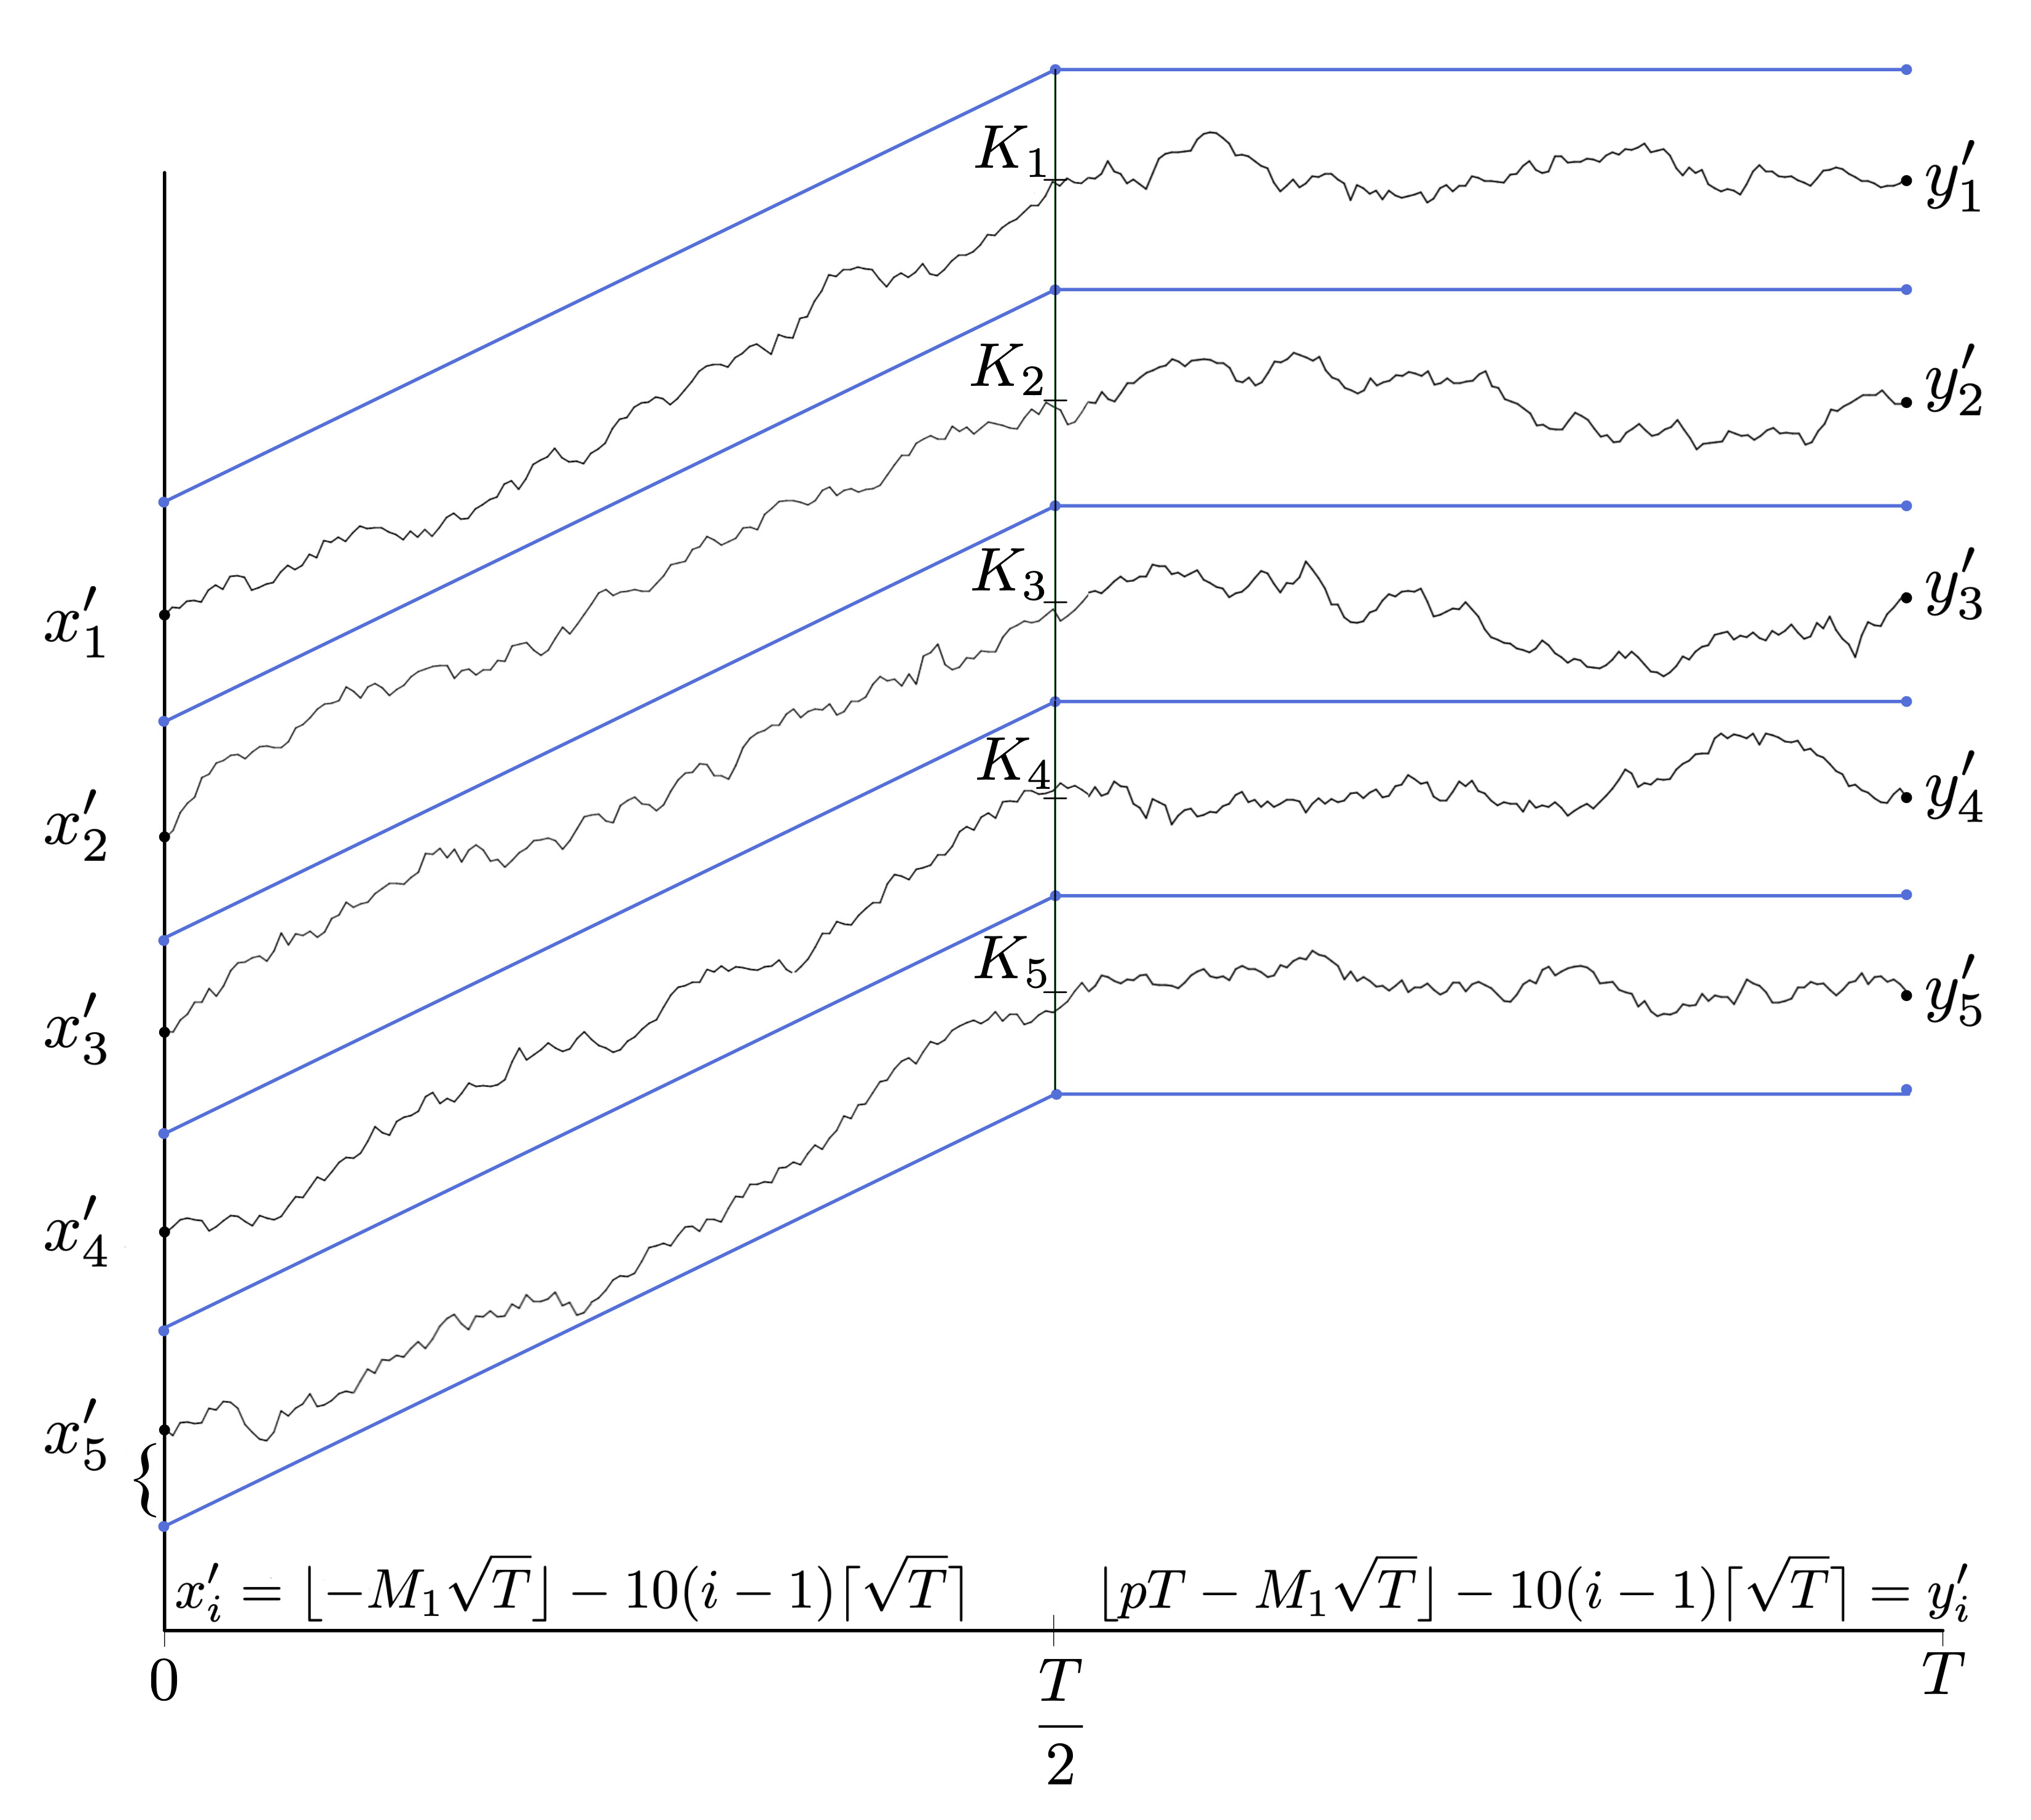
\includegraphics[width=0.85\textwidth]{graphics/Lemma320.jpg}{\kern 3em}
	\caption{Sketch of the argument for Lemma 3.20: \\We shift the Bernoulli random walks with entry and exit data $\vec x$ and $\vec y$ down to Bernoulli random walks with entry data $x'$ and $y'$, applying Monotone Coupling, Lemma \ref{MCLxy} to find that the probability of the even that midpoint of the random walk from $\vec x$ to $\vec y$ is greater than $M\sqrt{T}$ is greater  than the probability of the same event for random walks from $\vec x'$ to $\vec y'$. We then define the event $E$, which is the probability that each random walk lies within the blue bounding lines above after an affine shift. We may then use strong coupling with Brownian motions in accordance with Theorem \ref{KMT} to bound the  event $E$ from below, and use previously known results about Brownian motion to bound the original probability, the height of a random walk at its midpoint, from below.}
\end{figure}
	Let $\mathbb{P}$ be a probability space suporting a random variable $\ell^{(T,z)}$ with law $\mathbb{P}^{0,T,0,z}$ coupled with a Brownian bridge $B^\sigma$ with variance $\sigma^2$, as in Theorem \ref{KMT}. Then the last probability in brackets is bounded below by
	\begin{equation}\label{19BB}
	\begin{split}
	& \mathbb{P}^{0,T,0,z}_{Ber}\Big(\big|\ell(T/2)-pT/2-(M+M_1+5)\sqrt{T}\big|\leq 2\sqrt{T} - 5\quad\mathrm{and}\\
	&\qquad\qquad\qquad \sup_{s\in[0,T/2]}\Big|\ell(s)-ps-\frac{M+M_1+5}{\sqrt{T}/2}\,s\Big| \leq 3\sqrt{T} - 1 \quad\mathrm{and}\\
	&\qquad\qquad\qquad \sup_{s\in[T/2,T]}\Big|\ell(s)-ps-(M+M_1+5)\sqrt{T}+\frac{M+M_1+5}{\sqrt{T}/2}(s-T/2)\Big| \leq 3\sqrt{T} - 1 \Big)\\
	&\geq \mathbb{P}\Big(\big|\sqrt{T}\,B^\sigma_{1/2} - (M+M_1+5)\sqrt{T}\big|\leq \sqrt{T} \quad\mathrm{and}\\
	&\qquad\qquad\qquad\sup_{s\in[0,T/2]}\Big|\sqrt{T}\,B^\sigma_{s/T}-(M+M_1+5)\sqrt{T}\cdot\frac{s}{T/2}\Big| \leq 2\sqrt{T}\quad\mathrm{and}\\
	&\qquad\qquad\qquad \sup_{s\in[T/2,T]}\Big|\sqrt{T}\,B^\sigma_{s/T}-(M+M_1+5)\sqrt{T}\cdot\frac{T-s}{T/2}\Big| \leq 2\sqrt{T} \Big)\\
	&\qquad\qquad\qquad -  \mathbb{P}\Big(\Delta(T,z) > \sqrt{T}/2\Big).
	\end{split}
	\end{equation}
	Note that $B^\sigma_{1/2}$ is a centered Gaussian random variable with variance $p(1-p)/4 = \sigma^2(1/2)(1-1/2)$. Writing $\xi = B^\sigma_{1/2}$, it follows from Lemma \ref{2bridges} that there exist independent Brownian bridges $B^1,B^2$ with variance $\sigma^2/2$ so that $B^\sigma_s$ has the same law as $\frac{s}{T/2}\xi + B^1_{2s/T}$ for $s\in[0,T/2]$ and $\frac{T-s}{T/2}\xi + B^2_{(2s-T)/T}$ for $s\in[T/2,T]$. The first term in the last expression in \eqref{19BB} is thus equal to
	\begin{align*}
	&\mathbb{P}\Big(|\xi - (M+M_1+5)|\leq 1 \quad\mathrm{and} \sup_{s\in[0,T/2]}\Big|B^1_{s/T}-(M+M_1+5-\xi)\cdot\frac{s}{T/2}\Big| \leq 2\\
	&\qquad\qquad\qquad \mathrm{and}\quad \sup_{s\in[T/2,T]}\Big|B^2_{(2s-T)/T}-(M+M_1+5-\xi)\cdot\frac{T-s}{T/2}\Big| \leq 2 \Big)\\
	&\geq \mathbb{P}\Big(|\xi - (M+M_1+5)|\leq 1 \quad\mathrm{and} \sup_{s\in[0,T/2]}\big|B^1_{2s/T}\big| \leq 1 \qquad \mathrm{and}\quad \sup_{s\in[T/2,T]}\big|B^2_{(2s-T)/T}\big| \leq 1 \Big)\\
	&= \mathbb{P}\Big(|\xi-(M+M_1+5)|\leq 1\Big)\mathbb{P}\Big(\sup_{s\in[0,T/2]} \big|B^1_{2s/T}\big|\leq 1\Big)\mathbb{P}\Big(\sup_{s\in[0,T/2]} \big|B^2_{(2s-T)/T}\big|\leq 1\Big)\\
	&\geq \big(1-2e^{-4/p(1-p)}\big)^2 \int_{M+M_1+4}^{M+M_1+6} \frac{e^{-2\xi^2/p(1-p)}}{\sqrt{\pi p(1-p)/2}}\,d\xi\\
	&\geq \frac{2\sqrt{2}\,e^{-2(M+M_1+6)^2/p(1-p)}}{\sqrt{\pi p(1-p)}}\,\big(1-2e^{-4/p(1-p)}\big)^2.
	\end{align*}
	In the fourth line, we used the fact that $\xi$, $B^1_\cdot$, and $B^2_\cdot$ are independent, and in the second to last line, we used Lemma \ref{BBmax}. Since $|z-pT|\leq (M_1+1)\sqrt{T}$, Lemma \ref{Cheb} allows us to choose $T$ large enough so that $\mathbb{P}(\Delta(T,z) > \sqrt{T}/2)$ is less than 1/2 the last expression. Then in view of \eqref{19gibbs} and \eqref{19BB}, we conclude \eqref{19ineq}.
	
\end{proof}
\begin{lemma}\label{prob17}
Fix $p,t\in(0,1)$, $k\in\mathbb{N}$, $\vec a$, $\vec b\in W_k$.  Suppose that $\vec{x}^{T}=(x_{1}^{T},\cdots,x_{k}^{T})$ and $\vec{y}^{T}=(y_{1}^{T},\cdots,y_{k}^{T})$ are two sequence of $k$-dimensional vectors with integer entries such that for $i\in \llbracket 1,k\rrbracket$, $$\lim_{T\rightarrow\infty}\frac{x_{i}^{T}}{\sqrt{T}}=a_{i} \text{ and } \lim_{T\rightarrow\infty}\frac{y_{i}^{T}-pT}{\sqrt{T}}=b_{i}$$ and define the sequence of random $k$-dimensional vectors $Z^{T}$ by $$Z^{T}=\big(\frac{L_{1}(tT)-ptT}{\sqrt{T}},\cdots,\frac{L_{k}(tT)-ptT}{\sqrt{T}}\big),$$ where $(L_{1},\cdots,L_{k})$ is $\mathbb{P}^{0,T,\vec{x}^{T},\vec{y}^{T}}_{avoid,Ber}$-distributed. When $a_i=a_{i+1}$ or $b_{j}=b_{j+1}$ for any entries of $\vec a$ and $\vec b$, we write
\begin{equation*}\begin{split}
\vec{a}&=(a_{1},\cdots,a_{k})=(\underbrace{\alpha_{1},\cdots,\alpha_{1}}_{m_{1}},\cdots,\underbrace{\alpha_{p},\cdots,\alpha_{p}}_{m_{p}})\\
\vec{b}&=(b_{1},\cdots,b_{k})=(\underbrace{\beta_{1},\cdots,\beta_{1}}_{n_{1}},\cdots,\underbrace{\beta_{q},\cdots,\beta_{q}}_{n_{q}})
\end{split}
\end{equation*}
where $\alpha_{1}>\alpha_{2}>\cdots>\alpha_{p}$, $\beta_{1}>\beta_{2}>\cdots>\beta_{q}$ and $\sum_{i=1}^{p}m_{i}=\sum_{i=1}^{q}n_{i}=k$. Then, the random vector $Z^{T}$ converges weakly to a random variable $\hat Z$ with the density $$\rho_{\vec{a},\vec{b}}(z_{1},\cdots,z_{k})=\frac{1}{Z_{\vec{a},\vec{b}}}\cdot \varphi(\vec{a},\vec{z},\vec{m})\psi(\vec{b},\vec{z},\vec{n})\prod_{i=1}^{k}e^{-c_{3}(t,p)z_{i}^{2}}\mathbbm{1}_{\{z_{1}>\cdots> z_{k}\}}$$ where $\vec{m}=(m_{1},\cdots,m_{k})$, $\vec{n}=(n_{1},\cdots,n_{k})$, $c_{1},c_{2},c_{3}$ are constants depending on $p,t$ as given in Proposition \ref{WeakConvDistinct} , $Z_{\vec a,\vec b}$ is a constant depending on $p,t,\vec{a},\vec{b}$ such that $\rho_{\vec{a},\vec{b}}(z_{1},\cdots,z_{k})$ integrates to $1$ over $\mathbb{R}^{k}$, and $\varphi(\vec{a},\vec{z},\vec{m})$ and $\psi(\vec{b},\vec{z},\vec{n})$ are determinants:
\begin{equation*}
\varphi(\vec{a},\vec{z},\vec{m})= \det
\left[ \begin{array}{ccc}
((c_{1}(t,p)z_{j})^{i-1}e^{c_{1}(t,p)\alpha_{1}z_{j}})_{\substack{i=1,\cdots,m_{1}\\j=1,\cdots,k}}\\
\vdots\\
((c_{2}(t,p)z_{j})^{i-1}e^{c_{1}(t,p)\alpha_{p}z_{j}})_{\substack{i=1,\cdots,m_{p} \\j=1,\cdots,k}}
\end{array}
\right]
\end{equation*}
\begin{equation*}
\psi(\vec{b},\vec{z},\vec{n})= \det
\left[ \begin{array}{ccc}
((c_{2}(t,p)z_{j})^{i-1}e^{c_{2}(t,p)\beta_{1}z_{j}})_{\substack{i=1,\cdots,n_{1}\\j=1,\cdots,k}}\\
\vdots\\
((c_{2}(t,p)z_{j})^{i-1}e^{c_{2}(t,p)\beta_{q}z_{j}})_{\substack{i=1,\cdots, n_{q} \\j=1,\cdots,k}}
\end{array}
\right]
\end{equation*} 
\end{lemma}
Proof of this lemma will be postponed until the appendix, in propositions \ref{WeakConvDistinct} and \ref{WeakConvCollide}
\begin{lemma}\label{prob 20}
Fix $p,t\in (0,1)$ and $ k\in \mathbb{N}$. Suppose that $\vec x^T=(x_1^T,\cdots x_k^T)$ and $\vec y^T=(y_1^T,\cdots , y_k^T)$ is a sequence of $k$-dimensional vectors with integer entries such that $T\geq y_i^T-x_i^T\geq 0$ for $i\in \llbracket 1,k\rrbracket$. Show that for any $M_1,M_2>0$ and $\epsilon>0$ there exists $T_0\in\mathbb{N}$ and $\delta>0$ depending on $p,k,M_1,M_2$ such that if $T\geq T_0$, $\abs*{x_i^T}\leq M_1\sqrt{T}$ and $\abs*{y_i^T-pT}\leq M_2\sqrt{T}$ then 
\[
\pr^{0,T,\vec x^T, \vec y^T}_{avoid,Ber}\left(\min_{1\leq i\leq k-1} \left[L_i(tT)-L_{i+1}(tT)\right]<\delta\sqrt{T}\right)<\epsilon
\]
\end{lemma}
\begin{proof}
	We prove the claim by contradiction:
	suppose there exists $M_1,M_2,\epsilon>0$ such that for any $T_0\in \mathbb{N}$ and $\delta>0$ there exists some $T\geq T_0$ such that \[
	\pr^{0,T,\vec x^T,\vec y^T}_{avoid, Ber}\left(\min_{1\leq i\leq k-1}\left[L_i(tT)-L_{i+1}(tT)\right]<\delta\sqrt{T}\right)\geq \epsilon
	\]
	Therefore, we can obtain sequences $T_n$, $\delta_n>0$, $T_n\uparrow \infty$, $\delta_n\downarrow 0$ such that for all $n$, we have  
	\[
	\pr^{0,T,\vec x^{T_n},\vec y^{T_n}}_{avoid, Ber}\left(\min_{1\leq i\leq k-1}\left[\frac{L_i(tT_n)-L_{i+1}(tT_n)}{\sqrt{T_n}}\right]<\delta_n\right)\geq \epsilon
	\]
	As $\abs*{x_i^{T_n}}<M_1\sqrt{T_n}$, $\abs*{y_i^{T_n}-pT_n}\leq M_2\sqrt{T_n}$ we know that there exists some subsequence $T_{n_m}$ such that $\lim_{m\to\infty} \frac{x^{T_{n_m}}}{\sqrt{T_{n_m}}}\to \vec x$ 
	and 
	$\lim_{m\to\infty}\frac{y^{T_{n_m}}-pT}{\sqrt{T_{n_m}}}\to \vec y$ 
	by the Bolzano-Weierstrass theorem, as these sequences lie in compact intervals. Denote $$Z_i^m:=\frac{L_i(tT_{n_m})-ptT}{\sqrt{T_{n_m}}}.$$ Then, if we fix $\tilde\delta>0$, because $\delta_n\downarrow 0$, there exists some $M$ such that $m>M$ implies $\delta_m<\tilde\delta$. For such $m>M$, we have 
	\begin{equation}\label{prob20inf}
	\epsilon\leq \liminf_{m\to\infty}\pr\left(\min_{1\leq i\leq k-1}Z_i^m-Z_{i+1}^m<\delta_{n_m}\right)\leq \liminf_{m\to\infty}\pr\left(\min_{1\leq i\leq k-1}Z_i^m-Z_{i+1}^m\leq\tilde\delta\right)
	\end{equation}
	Now, if we apply the results of Lemma \ref{prob17}, we that the vector $(Z_1^m,\cdots, Z_k^m)$ converges weakly to some random vector $\hat Z$ with probability density function $\rho$ as defined previously in \ref{prob17}, the definitions of which we will state in a few lines, when  they are needed.
	Because this sequence has weak convergence we may apply portmanteau's lemma with the closed set $K=[0,\tilde\delta]$ to find 
	\begin{equation}\label{prob20sup}
	\limsup_{m\to\infty }\pr\left(\min_{1\leq i\leq k-1}Z_i^m-Z_{i+1}^m\in K\right)\leq \pr\left(\min_{1\leq i\leq k-1}\hat Z_i-\hat Z_{i+1}\in K\right)
	\end{equation}
	Combining (\ref{prob20inf}) and (\ref{prob20sup}), we arrive at the inequality
	\begin{equation}\label{eq:limsupinf}
	\epsilon\leq \liminf_{m\to\infty}\pr\left(\min_{1\leq i\leq k-1} Z_i^m-Z_{i+1}^m\leq \tilde\delta\right)\leq \pr\left(\min_{1\leq i\leq k-1} \hat Z_i-\hat Z_{i+1}\tilde\delta\right)
	\end{equation}
	and so by (\ref{eq:limsupinf}) and countable subadditivity,
	\begin{equation}\label{eq:ineq}
	\epsilon\leq \pr\left(\min_{1\leq i\leq k-1} \hat Z_i-\hat Z_{i+1}\leq\tilde\delta\right)\leq \sum_{i=1}^{k-1}\pr\left(\hat Z_i-\hat Z_{i+1}\leq \tilde\delta\right)
	\end{equation}
	
	Since $\tilde\delta$ is arbitrary, this inequality holds for any $\tilde\delta>0$. 
	In order to pick a sufficient $\delta'$ to find a contradiction, we will now state the definition of $\rho$, as found in \ref{prob17}: 
	\[\rho(z_1,\cdots ,z_k)=\frac{1}{Z_{\vec a, \vec b}}\cdot \varphi(\vec a, \vec z, \vec n)\cdot \psi(\vec b, \vec z, \vec n)\prod_{i=1}^{k}e^{\frac{-z_i^2}{t(1-t)}}
	\]
	with $\vec z_i\in W_k^\circ$ where we have the functions and constant
	\begin{align*}
	\varphi(\vec a,\vec z, \vec n)&=\det\begin{bmatrix}
	\left[(c_1(t,p)z_j)^{i-1}e^{c_1(t,p)\alpha_1 z_j}\right]_{\substack{i=1,...,m_1\\j=1,...,k}}\\
	\left[(c_1(t,p)z_j)^{i-1}e^{c_1(t,p)\alpha_2 z_j}\right]_{\substack{i=1,...,m_2\\j=1,...,k}}\\
	\vdots \\
	\left[(c_1(t,p)z_j)^{i-1}e^{c_1(t,p)\alpha_r z_j}\right]_{\substack{i=1,...,m_r\\j=1,...,k}}
	\end{bmatrix}\\
	\psi(\vec b, \vec z, \vec n)&=\det\begin{bmatrix}
	\left[(c_2(t,p)z_j)^{i-1}e^{c_2(t,p)\beta_1 z_j}\right]_{\substack{i=1,...,n_1\\j=1,...,k}}\\
	\left[(c_2(t,p)z_j)^{i-1}e^{c_2(t,p)\beta_2 z_j}\right]_{\substack{i=1,...,n_2\\j=1,...,k}}\\
	\vdots \\
	\left[(c_2(t,p)z_j)^{i-1}e^{c_2(t,p)\beta_q z_j}\right]_{\substack{i=1,...,n_q\\j=1,...,k}}
	\end{bmatrix}\\
	Z_{\vec a, \vec b}&=\int_{\mathbb{R}^k}\left(\indic_{z_1\geq z_2\geq \cdots \geq z_k}(\vec z)\right)\varphi(\vec a, \vec z, \vec n)\cdot \psi(\vec b, \vec z, \vec n)\prod_{i=1}^{k}e^{\frac{-z_i^2}{t(1-t)}} d\vec z
	\end{align*} we find that $\rho$ is continuous as a sum and product of continuous functions. Additionally, if for any $\chi\in\llbracket 1,k-1 \rrbracket$ such that $z_\chi=z_{\chi+1}$, then we have two equal columns 
	\[\begin{bmatrix}
	\left[(c_1(t,p)z_\chi)^{i-1}e^{c_1(t,p)\alpha_1 z_\chi}\right]_{i=1,...,m_1}\\
	\left[(c_1(t,p)z_\chi)^{i-1}e^{c_1(t,p)\alpha_2 z_\chi}\right]_{i=1,...,m_2}\\
	\vdots \\
	\left[(c_1(t,p)z_\chi)^{i-1}e^{c_1(t,p)\alpha_r z_\chi}\right]_{i=1,...,m_r}
	\end{bmatrix}=\begin{bmatrix}
	\left[(c_1(t,p)z_{\chi+1})^{i-1}e^{c_1(t,p)\alpha_1 z_{\chi+1}}\right]_{i=1,...,m_1}\\
	\left[(c_1(t,p)z_{\chi+1})^{i-1}e^{c_1(t,p)\alpha_2 z_{\chi+1}}\right]_{i=1,...,m_2}\\
	\vdots \\
	\left[(c_1(t,p)z_{\chi+1})^{i-1}e^{c_1(t,p)\alpha_r z_{\chi+1}}\right]_{i=1,...,m_r}
	\end{bmatrix}\]
	which implies that the determinant in $\varphi(\vec a,\vec b,\vec n)=0$, so $\rho(\vec z)=0$. Hence, if we let $E_i^\delta:=\{z\mid z_i-z_{i+1}\leq\delta\}$ we know by the continuity of $\rho$ that the accumulation function \[R_i(\delta):=\int_{E_i^\delta}\rho\] is well defined and continuous. We can find that $R_i(0)=\int_{E_i^0} 0$ by our previous calculation since $\rho=0$ on $E_i^0$ as $z_i=z_{i+1}$. By the continuity of $R$ we know that for any $\epsilon$ there exists a $\delta_i(\epsilon)$ such that $0<\delta<\delta_i(\epsilon)$ implies $|R_i(\delta)|<\epsilon$. Therefore, let $\tilde\delta=\min_{1\leq i\leq k-1}\delta_i\left(\frac\epsilon{k-1}\right)$ and we find that 
	\begin{equation}
	\label{prob20boundR}
	\pr\left( \hat Z_i-\hat Z_{i+1}\leq\tilde\delta \right)=R_i(\tilde\delta)<\frac{\epsilon}{k-1}
	\end{equation}
	for each integer $i\in \llbracket 1,k-1\rrbracket$. Combining equations (\ref{eq:ineq}) and (\ref{prob20boundR}) yields the inequality 
	\[\epsilon\leq \pr\left(\min_{1\leq i\leq k-1} \hat Z_i-\hat Z_{i+1}\leq\delta'\right)\leq \sum_{i=1}^{k-1}\pr\left(\hat Z_i-\hat Z_{i+1}\leq \delta'\right)< \epsilon
	\]
	which is a contradiction. Thus we have proved the Lemma.
\end{proof}
\begin{remark}
	Lemma \ref{prob 20} provides us with some amount of separation between the lines in the ensemble at any point along the Beroulli Random Walkers as $T$ tends to infinity. For any $\epsilon$, it allows us to find a distance $\delta$ such that the probability that any lines get closer than $\delta$ is less than $\epsilon$. The proof essentially passes to subsequential limits in order to use the convergence result of Lemma ($\ref{prob17}$), and then the fact that the density $\rho$ is continuous allows us to integrate $\rho(\vec z)$ over areas where $z_i$ values collide, and find that these integrals are $0$. Then we may use continuity around areas where $z_i$ values are equal to bound the probability where $z_i$ are close.
\end{remark}


%-------------------------------------------------------------------------------------------------------------------------------------------------------------------------------------------------
% Section 4
%
%-------------------------------------------------------------------------------------------------------------------------------------------------------------------------------------------------
\section{Proof of Theorem \ref{PropTightGood} }\label{Section4}


The goal of this section is to prove Theorem \ref{PropTightGood} and for the remainder we assume that $k \in \mathbb{N}$ with $k \geq 2$, $p \in (0,1)$, $\alpha, \lambda > 0$ are all fixed and 
\begin{equation}\label{eqalphagood}
\big\{\mathfrak{L}^N = (L^N_1,L^N_2, \dots, L^N_k)\big\}_{N=1}^{\infty},
\end{equation}
 is an $(\alpha,p,\lambda)$-good sequence of $\llbracket 1, k\rrbracket$-indexed Bernoulli line ensembles as in Definition \ref{Def1} that are all defined on a probability space with measure $\mathbb{P}$. The main technical result we will require is contained in Proposition \ref{PropMain} below and its proof is the content of Section \ref{Section4.1}. The proof of Theorem \ref{PropTightGood} is given in Section \ref{Section4.2}.
%-------------------------------------------------------------------------------------------------------------------------------------------------------------------------------------------------
% Section 4.1
%
%-------------------------------------------------------------------------------------------------------------------------------------------------------------------------------------------------
\subsection{Bounds on the acceptance probability}\label{Section4.1}
 The main result in this section is presented as Proposition \ref{PropMain} below. In order to formulate it and some of the lemmas below it will be convenient to adopt the following notation for any $r > 0$:
\begin{equation}\label{eqsts}
t_1 =\lfloor (r+1) N^{\alpha} \rfloor,\quad t_2 = \lfloor (r+2)N^{\alpha} \rfloor,\quad \textrm{and } t_3 = \lfloor (r+3)N^{\alpha} \rfloor.
\end{equation}
\begin{proposition}\label{PropMain} For any $\epsilon > 0$, $r > 0$ and any $(\alpha,p,\lambda)$-good sequence of Bernoulli line ensembles $\big\{ \mathfrak{L}^N  = (L^N_1,L^N_2, \dots, L^N_k)\big\}_{N=1}^{\infty}$
there exist $\delta > 0$ and $N_1$ (both depending on $\epsilon, r$ as well as $ \alpha, p, \lambda$ and the functions $\phi, \psi$ in Definition \ref{Def1}) such that for all $N \geq N_1$
we have 
$$\mathbb{P}\Big(Z\big( -t_1, t_1, \vec{x}, \vec{y} , L_{k}\llbracket -t_1, t_1\rrbracket\big) < \delta\Big) < \epsilon,$$
where $\vec{x} = (L_1^N(-t_1), \dots, L_{k-1}^N(-t_1)$, $\vec{y} = (L_1^N(t_1), \dots, L^N_{k-1}(t_1))$,  $ L_{k}\llbracket -t_1, t_1\rrbracket$ is the restriction of $L^N_k$ to the set $\llbracket -t_1, t_1\rrbracket$, and $Z$ is the acceptance probability of Definition \ref{DefAP}. $\mathbb{P}$ is the measure on a probability space that supports $\big\{ \mathfrak{L}^N \big\}_{N = 1}^\infty$.
\end{proposition}

The general strategy we use to prove Proposition \ref{PropMain} is inspired by the proof of Proposition 6.5 in \cite{CorHamK}. We begin by stating three key lemmas that will be required. Their proofs are postponed to Section \ref{Section5}. All constants in the statements below will depend implicitly on $\alpha$, $r$, $p$, $\lambda$, and the functions $\phi, \psi$ from Definition \ref{Def1}, which are fixed throughout. We will not list this dependence explicitly.

Lemma \ref{PropSup} controls the deviation of the curve $L^N_1(s)$ from the line $ps$ in the scale $N^{\alpha/2}$.
\begin{lemma}\label{PropSup} For each $\epsilon > 0$ there exist $R_1=R_1(\epsilon) > 0$ and $N_2= N_2(\epsilon)$ such that for $N \geq N_2$ 
$$\mathbb{P}\Big( \sup_{s \in [ -t_3, t_3] }\big( L^N_1(s) - p s \big) \geq  R_1N^{\alpha/2} \Big) < \epsilon.$$
\end{lemma}

Lemma \ref{PropSup2} controls the upper deviation of the curve $L^N_2(s)$ from the line $ps$ in the scale $N^{\alpha/2}$.
\begin{lemma}\label{PropSup2} For each $\epsilon > 0$ there exist $R_2=R_2( \epsilon) > 0$ and $N_3=N_3(\epsilon)$ such that for $N \geq N_3$
$$\mathbb{P}\Big( \inf_{s \in [ -t_2, t_2 ]}\big(L^N_k(s) - p s \big) \leq - R_2N^{\alpha/2} \Big) < \epsilon.$$
\end{lemma}

\begin{lemma}\label{LemmaAP1} Fix $k \in \mathbb{N}$, $p \in (0,1)$, $M_1, M_2 > 0$ . Suppose that $\ell_{bot}: \llbracket -t_2, t_2 \rrbracket \rightarrow \mathbb{R} \cup \{ - \infty \}$, and $\vec{x}, \vec{y} \in \mathfrak{W}_{k-1}$ are such that $2t_2 \geq y_i-x_i \geq 0$ for $i = 1, \dots, k-1$. Suppose further that
	\begin{enumerate}
		\item $\sup_{s \in [ -t_2,t_2]}\big(\ell_{bot}(s)  - ps \big)  \leq M_2 (2t_2)^{1/2}$,
		\item  $ x_{k-1} \geq \max\left(\ell_{bot}(t_2), pt_2- M_1 (2t_2)^{1/2}\right),$
		\item $ y_{k-1} \geq  \max \left( \ell_{bot}(t_2),  p t_2- M_1(2t_2)^{1/2} \right).$
	\end{enumerate}
	Define the constants $g$ and $h$ (depending on $ M_1, M_2, p , k, r$) via
	$$g =  \cdots \mbox{ and } h = \cdots .$$
	Then, there exists $N_4 = N_4(M_1,M_2,k ) \in \mathbb{N}$  such that for any $\tilde{\epsilon}  > 0$ and $N \geq N_4$ we have
	\begin{equation}\label{eqn60}
	\mathbb{P}^{-t_2, t_2, \vec{x},\vec{y}, \infty, \ell_{bot} }_{avoid, Ber} \Big( Z\big(  -t_1, t_1, Q(-t_1) ,Q(t_1), \ell_{bot}\llbracket -t_1, t_1\rrbracket\big) \leq  gh \tilde{\epsilon}   \Big)  \leq \tilde{\epsilon},
	\end{equation}
	where $\ell_{bot}\llbracket -t_1, t_1\rrbracket$ is the vector, whose coordinates match those of $\ell_{bot}$ on $\llbracket -t_1, t_1\rrbracket$ and $Q(a) = (Q_1(a), \dots, Q_{k-1}(a))$ is the value of the line ensemble $Q$ whose law is $\mathbb{P}^{-t_2, t_2, \vec{x},\vec{y}, \infty, \ell_{bot} }_{avoid, Ber}$ at location $a$.
\end{lemma}


\begin{proof}[Almost proof of Proposition \ref{PropMain}] Let $\epsilon > 0$ be given. Define the event
	\begin{equation*}
	\begin{split}
	&E_N = \Big\{    L_{k-1}^N(  \pm t_2) \mp pt_2 \geq  - M_1 (2t_2)^{1/2}\Big\} \cap \Big\{ \sup_{s \in [ -t_2, t_2]} \big( {L}^N_{k}(s) - p s \big)\leq M_2  (2t_2)^{1/2} \Big\},
	\end{split}
	\end{equation*}
	where $M_1$ and $M_2$ are sufficiently large so that for all large $N$ we have $\mathbb{P}(E_N^c) <  \epsilon / 2$. The existence of such $M_1$ and $M_2$ is assured from Lemmas \ref{PropSup} and \ref{PropSup2}. 
	
	Let $\delta = (\epsilon/2) \cdot g h$, where $g,h$ are as in Lemma \ref{LemmaAP1} for the values $M_1, M_2$ as above and $r$ as in the statement of the proposition.
	We denote
	$$V = \Big\{Z\big( -t_1,t_1, \vec{x}, \vec{y} , L_{k}\llbracket -t_1, t_1\rrbracket\big)< \delta\Big\}$$
	and make the following deduction
	\begin{equation*}
	\begin{split}
	&\mathbb{P}\big( V \cap E_N \big) =\mathbb{E} \bigg[    \mathbb{E}\Big[{\bf 1}_{E_N} \cdot {\bf 1}_{V} \Big{|} \mathcal{F}_{ext} \big( \{1, \dots, k-1\} \times \llbracket -t_2 + 1,t_2 - 1\rrbracket \big)\Big] \bigg] = \\
	&\mathbb{E} \bigg[ {\bf 1}_{E_N} \cdot   \mathbb{E}\Big[ {\bf 1} \{ Z\big( -t_1,t_1, \vec{x}, \vec{y} , L_{k}\llbracket -t_1, t_1\rrbracket \big) < \delta\}   \Big{|} \mathcal{F}_{ext} \big( \{1, \dots, k-1\} \times \llbracket -t_2 + 1,t_2 - 1\rrbracket \big)\Big] \bigg]  = \\
	&\mathbb{E} \left[ {\bf 1}_{E_N} \cdot  \mathbb{E}^{-t_2, t_2, L^N(-t_2), L^N(t_2), \infty, L^N_k\llbracket -t_2, t_2\rrbracket }_{avoid, Ber}\left[ {\bf 1} \{ Z\big( -t_1, t_1, \ell(-t_1),\ell(t_1),{L}^N_k\llbracket -t_1, t_1\rrbracket \big) < \delta\} \right] \right] \leq \\
	&  \mathbb{E} \left[ {\bf 1}_{E_N} \cdot  \epsilon/2 \right] \leq \epsilon/2.
	\end{split}
	\end{equation*}
	The first equality follows from the tower property for conditional expectations. The second equality uses the fact that ${\bf 1}_{E_N} $ is $\mathcal{F}_{ext} \big( \{1\} \times \llbracket -t_2 + 1,t_2 - 1\rrbracket$-measurable and can thus be taken outside of the conditional expectation as well as the definition of $V$. The third equality uses the Schur Gibbs property. The inequality on the third line uses Lemma \ref{LemmaAP1} with $\tilde{\epsilon} = \epsilon/2$ as well as the fact that on the event $E_N^c$ the random variables $L^N(-t_2), L^N(t_2)$ and $L^N_k \llbracket -t_2, t_2 \rrbracket$ (that play the roles of $\vec{x}, \vec{y}$ and $\ell_{bot}$) satisfy the inequalities 
	$$L^N_{k-1}(-t_2) \geq  -pt_2- M_1 (2t_2)^{1/2},  L^N_{k-1}(t_2) \geq  p t_2- M_1(2t_2)^{1/2}, \sup_{s \in [ -t_2,t_2]} \hspace{-2mm}\big(L^N_k(s)  - ps \big)  \leq M_2(2t_2)^{1/2}.$$
	The last inequality is trivial.
	
	Combining the above inequality with $\mathbb{P}(E_N^c) <  \epsilon/2$, we see that for all large $N$ we have
	$$\mathbb{P}\left( V  \right) = \mathbb{P}(V \cap E_N) + \mathbb{P}(V \cap E_N^c) \leq \epsilon/2 + \mathbb{P}(E_N^c) < \epsilon.$$
\end{proof}


%-------------------------------------------------------------------------------------------------------------------------------------------------------------------------------------------------
% Section 4.2
%
%-------------------------------------------------------------------------------------------------------------------------------------------------------------------------------------------------
\subsection{Proof of Theorem \ref{PropTightGood} }\label{Section4.2}
	
	By Lemma \ref{2Tight}, it suffices to verify the following two conditions for all $1\leq i\leq k$, $R>0$, and $\epsilon>0$:
	\begin{align}
	\lim_{a\to\infty} &\limsup_{N\to\infty} \pr(|f^N_i(0)|\geq a) = 0 \label{ThmCond1}\\
	\lim_{\delta\to 0} &\limsup_{N\to\infty} \pr\bigg(\sup_{\substack{x,y\in [-R,R], \\ |x-y|\leq\delta}} |f^N_i(x) - f^N_i(y)| \geq \epsilon\bigg)= 0. \label{ThmCond2}
	\end{align}
	For the sake of clarity, we will prove these conditions in two separate steps.\\
	
	\noindent\textbf{Step 1.} We first prove condition \eqref{ThmCond1}, making use of Lemmas \ref{PropSup} and \ref{PropSup2} in order to obtain upper and lower bounds for the top and bottom curves respectively, thus bounding all curves.
	
	Fix $\epsilon>0$. We show that there exists an $a>0$ and $N'$ such that $N>N'$ implies
	$$\pr(|f^N_i(0)|\geq a) = \pr(|L_i^N(0)|\geq a N^{\alpha/2})<\epsilon.$$
	By Lemmas \ref{PropSup} and \ref{PropSup2}, there exist $R_1 := R_1(\epsilon/2)>0$, $R_2 := R_2(\epsilon/2)>0$ and $N_2 := N_2(\epsilon/2),N_3 := N_3(\epsilon/2)$ such that 
	\begin{align*}
	N\geq N_2 &\text{ implies } \pr\Big(\sup_{s\in[-t_3,t_3]}\left(L_1^N(s)-ps\right)\geq R_1N^{\alpha/2}\Big)<\epsilon/2,\\
	N\geq N_3 &\text{ implies } \pr\Big(\inf_{s\in[-t_2,t_2]}\left(L_k^N(s)-ps\right)\leq -R_2 N^{\alpha/2}\Big)<\epsilon/2.
	\end{align*}
	In particular, taking $s=0$, we find that for $N\geq N' := N_2 \vee N_3$, 
	\begin{align*}
	\pr\big(L_1^N(0)\geq R_1N^{\alpha/2}\big) &\leq \pr\Big(\sup_{s\in[-t_3,t_3]}\left(L_1^N(s)-ps\right)\geq R_1N^{\alpha/2}\Big)< \epsilon/2,\\
	\pr\big(L_k^N(0)\leq -R_2N^{\alpha/2}\big) &\leq \pr\Big(\inf_{s\in[-t_2,t_2]}\left(L_k^N(s)-ps\right)\leq -R_2N^{\alpha/2}\Big)< \epsilon/2.
	\end{align*}
	Letting $a = R_1 \vee R_2$ and noting that $L_1^N(0)>L_2^N(0)>...>L_k^N(0)$, we find that for $1\leq i\leq k$ and $N \geq N'$,
	$$\pr\big(|L_i^N(0)|\geq a N^{\alpha/2}\big)\leq \pr\big(L_1^N(0)\geq R_1 N^{\alpha/2}\big) + \pr\big(L_k^N(0)\leq -R_2N^{\alpha/2}\big) < \epsilon.$$
	This proves \eqref{ThmCond1}.\\
	
	\noindent\textbf{Step 2.} Here, we will prove condition \eqref{ThmCond2} for a fixed $i$ in three parts. We must show that for all $\epsilon,\eta>0$ and $R>0$, there exists a $\delta$ and $N_0$ such that $N>N_0$ implies 
	\[
	\pr\bigg(\sup_{\substack{x,y\in [-R,R],\\ |x-y|\leq\delta}} |f^N_i(x) - f^N_i(y)| \geq \epsilon\bigg)<\eta.
	\]
	We rewrite the left hand side as
	\begin{align}
	\pr\bigg(\sup_{\substack{x,y\in [-R,R],\\ |x-y|\leq\delta}} \abs*{N^{-\alpha/2}\left(L^N_i(xN^{\alpha}) - L^N_i(yN^\alpha)\right)-p(x-y)N^{\alpha/2}+\lambda(x^2-y^2)} \geq \epsilon\bigg).
	\end{align}
	Given that $|x-y|<\delta$ and $x,y\in [-R,R]$, we know that $|x+y|\leq 2R$ and $|x-y|<\delta$, hence $|x^2-y^2|\leq 2R\delta$. Thus if we take $\delta < \frac{\epsilon}{8\lambda R}$, then the last probability is bounded below by
	\begin{align*}
	&\pr\bigg(\sup_{\substack{x,y\in [-R,R],\\ |x-y|\leq\delta}} N^{-\alpha/2}\abs*{L_i^N(xN^\alpha)-L_i^N(yN^\alpha)-p(x-y)N^\alpha}+2\lambda R\delta\geq \epsilon\bigg)\\
	\leq \; & \pr\bigg(\sup_{\substack{x,y\in [-R,R],\\ |x-y|\leq\delta}} \abs*{L_i^N(xN^\alpha)-L_i^N(yN^\alpha)-p(x-y)N^\alpha}\geq \frac{3N^{\alpha/2}\epsilon}4\bigg)\\
	= \; & \pr\bigg(\sup_{\substack{x,y\in [-RN^\alpha,RN^\alpha],\\ |x-y|\leq \delta N^\alpha}} \abs*{L_i^N(x)-L_i^N(y)-p(x-y)}\geq \frac{3N^{\alpha/2}\epsilon}4\bigg).
	\end{align*}
	We denote the event in the last line by $A_\delta$, and we now bound $\mathbb{P}(A_\delta)$ by size-biasing.
	
	Define events
	\begin{align*}
	E_1&=\left\{\max_{1\leq j \leq i}\abs*{f_j(\pm R)}\leq M_1\right\},\\
	E_2&=\left\{Z(-RN^\alpha, RN^\alpha, \vec x, \vec y, \infty, L_{i+1}^N[-RN^\alpha, RN^\alpha])>\delta_1\right\}.
	\end{align*}
	Here, $\vec{x} = (L_1^N(-RN^\alpha),\dots,L_i(-RN^\alpha))$ and $\vec{y} = (L_1^N(RN^\alpha),\dots,L_i(RN^\alpha))$. We argue that $E_1,E_2$ have high probability for appropriately chosen $M_1,\delta_1$, and it then suffices to bound the probability of $A_\delta$ on these events.
	
	Firstly, we observe that $L_j^N(\pm RN^\alpha)> L_{j+1}^N(\pm RN^\alpha)$, so $f_j^N(\pm R)>f_{j+1}^N(\pm R)$ as well. Thus
	\begin{align*}
	E_1^c &= \{f_1(\pm R)> M_1\} \cup \{f_i(\pm R)<-M_1\} \\
	&= \left\{ \left(L_1^N(\pm RN^\alpha)\mp pRN^\alpha\right)> (M_1-\lambda R^2)N^{\alpha/2}\right\}\\
	&\qquad \cup \left\{\left(L_i^N(\pm RN^\alpha)\mp pRN^\alpha\right)< -(\lambda R^2+M_1)N^{\alpha/2}\right\}.
	\end{align*}
	Now take $r>R$. Then in particular $RN^\alpha \leq t_3$, so we have $$
	\pr\left(L_1^N(\pm RN^\alpha)\mp prN^\alpha>(M_1-\lambda R^2)N^{\alpha/2}\right)
	\leq\pr\Big(\sup_{s\in[-t_3,t_3]}L_1^N(s)-ps>(M_1-\lambda R^2)N^{\alpha/2}\Big).
	$$ By Lemma \ref{PropSup}, we find that if $M_1>R_1(\eta/8)+\lambda R^2$ and $N>N_1(\eta/8)$, then this probability is less than $\eta/8$. Next, we have
	\begin{align*}
	\pr \left(L_i^N(\pm RN^\alpha)\mp pRN^\alpha< -(\lambda R^2+M_1)N^{\alpha/2}\right)&\leq \pr \left(L_i^N(\pm RN^\alpha)\mp pRN^\alpha< -M_1N^{\alpha/2}\right)\\
	&\leq \pr\Big(\inf_{s\in[-t_2,t_2]}\big(L_i^N(s)-ps\big)<-M_1N^{\alpha/2}\Big),
	\end{align*}
	and this last probability is $<\eta/8$ for $M_1\geq R_2(\eta/8)$ and $N>N_2(\eta/8)$ by Lemma \ref{PropSup2}. Therefore taking $M_1=\max\{R_1(\eta/8)+\lambda R^2,R_2(\eta/8)\}$, we find $$\pr(E_1^c)<\frac{\eta}{4}.$$
	Now by Proposition \ref{PropMain} with $r=R-1$, there exist $\delta_1(\eta/4)$ and $N_1(\eta/4)$ such that $N\geq N_1$ implies 
	\[
	\pr\left( E_2^c\right)<\frac{\eta}{4}.
	\]
	In summary, for $N>N_{01} := \max\{N_1(\eta/4),N_2(\eta/8),N_3(\eta/8)\}$, 
	\begin{equation}
	\pr(A_\delta)= \pr(A_\delta\cap E_1\cap E_2)+\pr(A_\delta\cap\left(E_1^c\cup E_2^c\right))\leq \pr(A_\delta\cap E_1\cap E_2)+\frac{\eta}{2}. \label{ThmBias}
	\end{equation}
	It remains to bound the first term. We define a $\sigma$-algebra 
	$$\mathcal{F}=\sigma\left(L_{i+1}^N,L_1^N(\pm RN^\alpha ), L_2^N(\pm RN^\alpha ),\dots, L_i^N(\pm RN^\alpha )\right).$$
	Clearly $E_1, E_2\in \mathcal{F}$, so the indicator random variables $\indic_{E_1}$ and $\indic_{E_2}$ are $\mathcal{F}$-measurable. It follows from the tower property of conditional expectation that
	\begin{align}
	\pr(A_\delta\cap E_1\cap E_2)&=\ex[\indic_{A_\delta} \indic_{E_1} \indic_{E_2}] =\ex[\indic_{E_1} \indic_{E_2}\ex[\indic_{A_\delta}\mid \mathcal{F}]\,]. \label{tower}
	\end{align}
	By the Schur-Gibbs property (see Definition \ref{DefSGP}),
	\[
	\ex[\indic_{A_\delta}\mid \mathcal{F}]=\ex_{avoid,Ber}^{-RN^\alpha,RN^\alpha,\vec x, \vec y, \infty, L_{i+1}^N}[\indic_{A_\delta}].
	\]
	We now observe that the Radon-Nikodym derivative of $\pr_{avoid,Ber}^{-RN^\alpha,RN^\alpha,\vec x, \vec y, \infty, L_{m+1}^N}$ with respect to $\pr_{Ber}^{-RN^\alpha, RN^\alpha,\vec x,\vec y}$ is given by 
	\begin{equation}
	\frac{d\pr_{avoid,Ber}^{-RN^\alpha,RN^\alpha,\vec x, \vec y, \infty, L_{i+1}^N}}{d\pr_{Ber}^{-RN^\alpha, RN^\alpha,\vec x,\vec y}} = \frac{\indic_{\left\{L_1 \geq \cdots \geq L_{i+1}\right\}}}{Z(-RN^\alpha,RN^\alpha,\vec x, \vec y, L_{i+1}^N)}. \label{RN}
	\end{equation}
	To see this, note that for any event $A$,
	\begin{align*}
	&\pr_{avoid,Ber}^{-RN^\alpha,RN^\alpha,\vec x, \vec y, \infty, L_{i+1}^N}(A) = \frac{\pr_{Ber}^{-RN^\alpha,RN^\alpha,\vec x, \vec y}(A\cap\left\{L_1 \geq \cdots \geq L_{i+1}\right\})}{\pr_{Ber}^{-RN^\alpha,RN^\alpha,\vec x, \vec y}(L_1\geq\cdots\geq L_{i+1})}\\
	= \; & \frac{\ex_{Ber}^{-RN^\alpha,RN^\alpha,\vec x, \vec y}\left[\indic_A \indic_{\left\{L_1\geq\cdots\geq L_{i+1}\right\}}\right]}{Z(-RN^\alpha,RN^\alpha,\vec{x},\vec{y},L^N_{i+1})} = \int_A \frac{\indic_{\left\{L_1\geq\cdots\geq L_{i+1}\right\}}}{Z(-RN^\alpha,RN^\alpha,\vec x, \vec y, L_{i+1}^N)}\,d\pr_{Ber}^{-RN^\alpha,RN^\alpha,\vec x, \vec y}.
	\end{align*}
	It follows from \eqref{tower}, \eqref{RN}, and the definition of $E_2$ that
	\begin{align*}
	\pr(A_\delta\cap E_1\cap E_2) &=\ex\left[\indic_{E_1}\indic_{E_2} \ex_{Ber}^{-RN^\alpha, RN^\alpha,\vec x,\vec y}\left[\frac{\indic_{A_\delta}\cdot \indic_{\left\{L_1\geq\cdots\geq L_{i+1}\right\}}}{Z(-RN^\alpha,RN^\alpha,\vec x, \vec y, L_{i+1}^N)}\right]\right]\\
	&\leq \ex\left[\indic_{E_1}\ex_{Ber}^{-RN^\alpha,RN^\alpha,\vec x,\vec y}\left[\frac{\indic_{A_\delta}}{\delta_1}\right]\right]\\
	&\leq \frac{1}{\delta_1}\,\pr_{Ber}^{-RN^\alpha,RN^\alpha,\vec x,\vec y}(A_\delta).
	\end{align*}
	By Lemma \ref{MOCLemmaS4}, there exist $N_4$ and $\delta$ such that $N>N_4$ implies
	\[
	\pr_{Ber}^{-RN^\alpha,RN^\alpha,\vec x,\vec y}(A_\delta)<\frac{\eta\,\delta_1}2,
	\] 
	and hence $$\pr\left(A_\delta\cap E_1\cap E_2\right)\leq \frac{\eta}{2}.$$ We conclude from \eqref{ThmBias} that $\mathbb{P}(A_\delta) < \eta$ for $N\geq N_0 := N_{01} \vee N_4$. This completes the proof.



%-------------------------------------------------------------------------------------------------------------------------------------------------------------------------------------------------
%    Section 5
%
%-------------------------------------------------------------------------------------------------------------------------------------------------------------------------------------------------
\section{Proof of three key lemmas}\label{Section5}
Here we prove the three key lemmas from Section \ref{Section4.1}.

\subsection{Proof of Lemma \ref{PropSup}}

We first establish some notation. Let $a,b,t_1,t_2,z_1,z_2 \in \mathbb{Z}$ be given such that $t_1 + 1 < t_2$, $0\leq z_2 - z_1 \leq t_2 - t_1$, $0\leq b-a \leq t_2 - t_1$, $z_1\leq a$, and $z_2\leq b$. We write $\ell\in\Omega(t_1,t_2,a,b)$ and $\ell_{bot}\in\Omega(t_1,t_2,z_1,z_2)$ for generic paths in these two spaces, and we consider the event $\{\ell \geq \ell_{bot}\} = \{\ell(s) \geq \ell_{bot}(s), s\in[t_1,t_2]\}$. Note that $\mathbb{P}^{t_1,t_2,a,b,\infty,\ell_{bot}}_{avoid,Ber}(\ell) = \mathbb{P}^{t_1,t_2,a,b}_{Ber}(\ell\,|\,\ell \geq \ell_{bot}))$. We now establish some auxiliary results which will be used in the proof of Lemma \ref{PropSup}.

\begin{lemma}\label{pathcounting}
	If $a\leq k_1\leq k_2\leq a + T - t_1$, then with notation as above,
	\[
	\mathbb{P}^{t_1, t_2, a, b}_{Ber}\big( \ell \geq \ell_{bot}\,\big|\,\ell(T) = k_1\big) \leq \mathbb{P}^{t_1, t_2, a, b}_{Ber}\big(\ell \geq \ell_{bot}\,\big|\,\ell(T) = k_2\big).
	\]
\end{lemma}

\begin{remark}
	This lemma essentially states that a path $\ell$ is more likely to lie above $\ell_{bot}$ if its value at a point $T$ is increased. A more general result is proven in \cite[Lemma 4.1]{CD}
\end{remark}

\begin{proof}
	Let $\ell_1$ be a random path distributed according to $\mathbb{P}^{t_1, t_2, a, b}_{Ber}$ conditioned on $\ell_1(T) = k_1$. We can identify $\ell_1$ with a sequence of $+$'s and $-$'s of length $t_2-t_1$, where a $+$ in the $i$th position means that $\ell_1(t_1+i+1)-\ell_1(t_1+i) = 1$, and a $-$ means that $\ell_1(t_1+i+1)-\ell_1(t_1+i) = 0$. [Maybe include Figure 9 from Corwin-Dimitrov here.] In this representation, the value of $\ell_1(T)$ is $a$ plus the number of $+$'s in the first $T-t_1$ slots, and the value of $\ell_1(t_2)$ is $a$ plus the total number of $+$'s. Note that we must have exactly $(k_1-a)$ $+$'s in the first $T-t_1$ slots, and $(b-k_1)$ $+$'s in the last $t_2-T$ slots. We pick uniformly at random $(k_2-k_1)$ $-$'s in the first $T-t_1$ slots and change them to $+$'s, then pick randomly $(k_2-k_1)$ $+$'s in the last $t_2-T$ slots and change them to $-$'s. This defines a new path $\ell_2$. Since there are now $k_2-a$ $+$'s in the first $T-t_1$ slots, we have $\ell_2(T) = k_2$, and we still have $\ell_2(t_2) = b$ since the number of $+$'s is unchanged. Thus we see that $\ell_2$ is distributed according to $\mathbb{P}^{t_1,t_2,a,b}_{Ber}$ conditioned on $\ell_2(T) = k_2$. 
	
	Now suppose $\ell_1 \geq \ell_{bot}$. We claim that $\ell_2 \geq \ell_1$ on all of $[t_1,t_2]$. To see this, note that for any $s\in\llbracket t_1, t_2\rrbracket$, $\ell_2(s) - \ell_1(s)$ is equal to the number of $+$'s in the first $s-t_1$ slots of the sequence representing $\ell_2$, minus the corresponding number for $\ell_1$. If $s\leq T$, this difference is clearly positive by construction. The difference is equal to $k_2 - k_1 \geq 0$ at $s = T$, and the difference then decreases monotonically as $s$ increases to $t_2$, since we have removed exactly $k_2-k_1$ $+$'s from the last $t_2-T$ slots. The difference is of course 0 at $s = t_2$, so this proves the claim. It follows that
	\[
	\mathbf{1}_{\ell_1 \geq \ell_{bot}} \leq \mathbf{1}_{\ell_2 \geq \ell_{bot}}.
	\]
	Now taking expectations of both sides and recalling the distributions of $\ell_1,\ell_2$ proves the lemma.
\end{proof}


\begin{corollary}\label{setpathcounting}
	Let $T\in\llbracket t_1, t_2\rrbracket$, and let $A, B$ be nonempty sets of integers such that $a \leq \alpha \leq \beta \leq a+T-t_1$ for all $\alpha\in A, \beta\in B$. Then
	\[
	\mathbb{P}^{t_1, t_2, a, b}_{Ber}\big(\ell \geq \ell_{bot}\,\big|\,\ell(T) \in A\big) \leq \mathbb{P}^{t_1, t_2, a, b}_{Ber}\big(\ell \geq \ell_{bot}\,\big|\,\ell(T) \in B\big).
	\]
\end{corollary}

\begin{proof}
	We have
	\begin{align*}
	& \mathbb{P}^{t_1, t_2, a, b}_{Ber}\big(\ell \geq \ell_{bot}\,\big|\,\ell(T) \in A\big) = \sum_{\alpha\in A} \mathbb{P}^{t_1, t_2, a, b}_{Ber}\big(\ell \geq \ell_{bot}\,\big|\,\ell(T) = \alpha\big) \cdot \frac{\mathbb{P}^{t_1, t_2, a, b}_{Ber}(\ell(T) = \alpha)}{\mathbb{P}^{t_1, t_2, a, b}_{Ber}(\ell(T) \in A)}\\
	= \; & \sum_{\alpha\in A}\sum_{\beta\in B} \mathbb{P}^{t_1, t_2, a, b}_{Ber}\big(\ell \geq \ell_{bot}\,\big|\,\ell(T) = \alpha\big) \cdot \frac{\mathbb{P}^{t_1, t_2, a, b}_{Ber}(\ell(T) = \alpha)}{\mathbb{P}^{t_1, t_2, a, b}_{Ber}(\ell(T) \in A)} \cdot \frac{\mathbb{P}^{t_1, t_2, a, b}_{Ber}(\ell(T) = \beta)}{\mathbb{P}^{t_1, t_2, a, b}_{Ber}(\ell(T) \in B)}\\
	\leq \; & \sum_{\alpha\in A}\sum_{\beta\in B} \mathbb{P}^{t_1, t_2, a, b}_{Ber}\big(\ell \geq \ell_{bot}\,\big|\,\ell(T) = \beta\big) \cdot \frac{\mathbb{P}^{t_1, t_2, a, b}_{Ber}(\ell(T) = \alpha)}{\mathbb{P}^{t_1, t_2, a, b}_{Ber}(\ell(T) \in A)} \cdot \frac{\mathbb{P}^{t_1, t_2, a, b}_{Ber}(\ell(T) = \beta)}{\mathbb{P}^{t_1, t_2, a, b}_{Ber}(\ell(T) \in B)}\\
	= \; & \sum_{\beta \in B} \mathbb{P}^{t_1, t_2, a, b}_{Ber}\big(\ell \geq \ell_{bot}\,\big|\,\ell(T) = \beta\big) \cdot \frac{\mathbb{P}^{t_1, t_2, a, b}_{Ber}(\ell(T) = \beta)}{\mathbb{P}^{t_1, t_2, a, b}_{Ber}(\ell(T) \in B)} = \mathbb{P}^{t_1, t_2, a, b}_{Ber}\big(\ell \geq \ell_{bot}\,\big|\,\ell(T) \in B\big).
	\end{align*}
	The inequality in the third line follows from Lemma \ref{pathcounting}.
\end{proof}

\begin{corollary}\label{freeavoidbound}
	Let $\alpha \leq a + T - t_1$. Then
	\begin{align*}
	\mathbb{P}^{t_1,t_2,a,b,\infty,\ell_{bot}}_{avoid,Ber} (\ell(T)\geq\alpha) &\geq \mathbb{P}^{t_1,t_2,a,b}_{Ber} (\ell(T)\geq \alpha).
	\end{align*}
\end{corollary}

\begin{proof}
	We write $\mathbb{P} := \mathbb{P}^{t_1,t_2,a,b}_{Ber}$ for brevity. Using Bayes' theorem repeatedly, we find
	\begin{align*}
	\mathbb{P}(\ell(T)\geq\alpha\,|\,\ell \geq \ell_{bot}) &= \frac{\mathbb{P}(\ell \geq \ell_{bot}\,|\,\ell(T)\geq\alpha) \mathbb{P}(\ell(T)\geq\alpha)}{\mathbb{P}(\ell \geq \ell_{bot})}\\ 
	&\geq \frac{\mathbb{P}(\ell \geq \ell_{bot}\,|\,\ell(T) < \alpha) \mathbb{P}(\ell(T)\geq\alpha)}{\mathbb{P}(\ell \geq \ell_{bot})}\\
	&= \big(1 - \mathbb{P}(\ell(T)\geq\alpha\,|\,\ell \geq \ell_{bot})\big)\cdot\frac{\mathbb{P}(\ell(T)\geq\alpha)}{\mathbb{P}(\ell(T) < \alpha)}.
	\end{align*}
	The inequality in the second line follows from Corollary \ref{setpathcounting}. It follows that
	\[
	\mathbb{P}(\ell(T)\geq\alpha\,|\,\ell \geq \ell_{bot}) \geq \frac{\mathbb{P}(\ell(T)\geq\alpha)}{\mathbb{P}(\ell(T)\geq\alpha) + \mathbb{P}(\ell(T) < \alpha)} = \mathbb{P}(\ell(T)\geq\alpha).
	\]
\end{proof}

We are now ready to prove Lemma \ref{PropSup}. The proof is similar to that of \cite[Lemma 5.2]{CD}. We exploit the one-point tightness of $L_1^N$ at two appropriately chosen points, and we use Lemma \ref{LemmaHalfS4} to control the deviation of $L_1^N$ from the line of slope $p$ away from these points.

\begin{proof}
	We write $s_4 = \lceil r+3 \rceil N^\alpha$, $s_3 = \lfloor r+3 \rfloor N^\alpha$, so that $s_3 \leq t_3 \leq s_4$, and take $N$ large enough so that $L_1^N$ is defined at $s_4$. We define events 
	\[
	E(M) = \Big\{\big|L_1^N(-s_4) + ps_4\big| > MN^{\alpha/2}\Big\}, \quad F(M) = \Big\{L_1^N(-s_3) > -ps_3 + MN^{\alpha/2} \Big\},
	\]
	\[
	G(M) = \Bigg\{\sup_{s\in[0,t_3]} \big(L_1^N(s) - ps \big) \geq (6r+22)(2r+6)^{1/2}(M+1)N^{\alpha/2} \Bigg\}.
	\]
	For $a,b\in\mathbb{Z}$, $s\in\llbracket 0, t_3 \rrbracket$, and $\ell_{bot}\in\Omega(-s_4,s,z_1,z_2)$ with $z_1\leq a$, $z_2\leq b$, we also define $E(a,b,s,\ell_{bot})$ to be the event that $L_1^N(-s_4) = a$, $L_1^N(s) = b$, and $L_2^N$ agrees with $\ell_{bot}$ on $[-s_4,s]$. 
	
	We claim that the set $G(M) \setminus E(M)$ can be written as a \textit{countable disjoint} union of sets $E(a,b,s,\ell_{bot})$. Let $D(M)$ be the set of tuples $(a,b,s,\ell_{bot})$ satisfying
	\begin{enumerate}[label=(\arabic*)]
		
		\item $0\leq s\leq t_3$,
		
		\item $0\leq b-a \leq s + s_4$, $|a + ps_4| \leq MN^{\alpha/2}$, and $b-ps > (6r+22)(2r+6)^{1/2}(M+1)N^{\alpha/2}$,
		
		\item $z_1\leq a, z_2\leq b$, and $\ell_{bot}\in\Omega(-s_4, s, z_1, z_2)$.
		
	\end{enumerate}
	Conditions (1) and (2) show that the union of these sets $E(a,b,s,\ell_{bot})$ for $(a,b,s,\ell_{bot})\in D(M)$ is $G(M)\setminus E(M)$. Observe that $D(M)$ is countable, since there are finitely many possible choices of $s$, countably many $a,b$ and $z_1,z_2$ for each $s$, and finitely many $\ell_{bot}$ for each $z_1,z_2$. Moreover, the sets $E(a,b,s,\ell_{bot})$ are clearly pairwise disjoint for distinct tuples in $D(M)$. This proves the claim.
	
	Now by one-point tightness of $L_1^N$ at integer multiples of $N^\alpha$, we can choose $M$ large enough depending on $\epsilon$ so that
	\begin{equation}
	\mathbb{P}(E(M)) < \epsilon/4, \quad \mathbb{P}(F(M)) < \epsilon/12 \label{4.2EFbounds}
	\end{equation}
	for all $N\in\mathbb{N}$. If $(a,b,s,\ell_{bot})\in D(M)$, then
	\begin{align*}
	\mathbb{P}^{-s_4,s,a,b}_{Ber}\Big( \ell(-s_3) > -ps_3 + MN^{\alpha/2}\Big) &= \mathbb{P}^{0,s+s_4,0,b-a}_{Ber}\Big(\ell(s_4-s_3) + a \geq -ps_3 + MN^{\alpha/2}\Big)\\
	&\geq \mathbb{P}^{0,s+s_4,0,b-a}_{Ber}\Big(\ell(s_4-s_3) \geq p(s_4-s_3) + 2MN^{\alpha/2}\Big).
	\end{align*}
	The inequality follows from the assumption in (2) that $a+ps_4 \geq -MN^{\alpha/2}$. Moreover, since $b-ps > (6r+22)(2r+6)^{1/2}(M+1)N^{\alpha/2}$ and $a+ps_4 \leq MN^{\alpha/2}$, we have 
	\[
	b-a \geq p(s+s_4) + (6r+21)(2r+6)^{1/2}(M+1)N^{\alpha/2} \geq p(s+t_3) + (6r+21)(M+1)(s+s_4)^{1/2}.
	\]  
	The second inequality follows since $s+s_4 \leq 2s_4 \leq (2r+6)N^{\alpha}$. It follows from Lemma \ref{LemmaHalfS4} with $M_1 = 0$, $M_2 = (6r+21)(M+1)$ that for sufficiently large $N$, we have
	\begin{equation}
	\mathbb{P}^{0,s+s_4,0,b-a}_{Ber}\Big(\ell(s_4-s_3) \geq \frac{s_4-s_3}{s+s_4}[p(s+s_4) + M_2 N^{\alpha/2}] - (s+s_4)^{1/4}\Big) \geq 1/3, \label{4.2interp}
	\end{equation}
	for all $(a,b,s,\ell_{bot}) \in D(M)$ simultaneously. Note that $\frac{s_4-s_3}{s+s_4} \geq \frac{N^\alpha - 1}{(2r+6)N^\alpha} \geq \frac{1}{2r+7}$
	for large $N$. Hence $\frac{s_4-s_3}{s+s_4}[p(s+t_3) + M_2 N^{\alpha/2}] - (s+s_4)^{1/4} \geq p(s+s_4) + 3(M+1)N^{\alpha/2} - (s+s_4)^{1/4}\geq p(s+s_4) + 2MN^{\alpha/2}$ for all large enough $N$. We conclude from \eqref{4.2interp} that
	\[
	\mathbb{P}^{-s_4,s,a,b}_{Ber}\Big(\ell(-s_3) > -ps_3 + MN^{\alpha/2}\Big) \geq 1/3
	\]
	uniformly in $a,b$ for large $N$. Now by the Gibbs property for $L^N$, we have for any $\ell\in\Omega(-s_4,s,a,b)$ that
	\[
	\mathbb{P}(L_1^N|_{[-s_4,s]} = \ell\,|\,E(a,b,s,\ell_{bot})) = \mathbb{P}^{-s_4,s,a,b,\infty,\ell_{bot}}_{avoid, Ber}(\ell).
	\]
	Hence by Corollary \ref{freeavoidbound},
	\begin{align*}
	&\mathbb{P}\big( L_1^N(-s_3) > -ps_3 + MN^{\alpha/2}\,\big|\,E(a,b,s,\ell_{bot})\big)\\
	= \; & \sum_{\ell\in\Omega(-s_4,s,a,b)} \mathbb{P}^{-s_4,s,a,b,\infty,\ell_{bot}}_{avoid, Ber}(\ell)\cdot \mathbb{P}^{-s_4,s,a,b,\infty,\ell_{bot}}_{avoid, Ber}\big(\ell(-s_3) > -ps_3 + MN^{\alpha/2}\big)\\
	\geq \; & \sum_{\ell\in\Omega(-s_4,s,a,b)} \mathbb{P}^{-s_4,s,a,b,\infty,\ell_{bot}}_{avoid, Ber}(\ell)\cdot \mathbb{P}^{-s_4,s,a,b}_{Ber}\big(\ell(-s_3) > -ps_3 + MN^{\alpha/2}\big)\\
	\geq \; & \frac{1}{3}\sum_{\ell\in\Omega(-s_4,s,a,b)} \mathbb{P}^{-s_4,s,a,b,\infty,\ell_{bot}}_{avoid, Ber}(\ell) = \frac{1}{3}.
	\end{align*}
	Note once again that this bound holds independent of $a,b$ for all sufficiently large $N$. It follows from \eqref{4.2EFbounds} that
	\[
	\epsilon/12 > \mathbb{P}(F(M)) \geq \sum_{(a,b,s,\ell_{bot})\in D(M)} \mathbb{P}(F(M)\cap E(a,b,s,\ell_{bot}))
	\]
	\[
	= \sum_{(a,b,s,\ell_{bot})\in D(M)} \mathbb{P}(F(M)\,|\, E(a,b,s,\ell_{bot}))\mathbb{P}(E(a,b,s,\ell_{bot})) \geq \frac{1}{3}\mathbb{P}(G(M)\setminus E(M))
	\]
	for large $N$. Since in addition $\mathbb{P}(E(M)) < \epsilon/4$, we find that
	\[
	\mathbb{P}\Big( \sup_{s \in [0,t_3] }\big( L^N_1(s) - p s \big) \geq  (6r+22)(2r+6)^{1/2}(M+1)N^{\alpha/2} \Big) = \mathbb{P}(G(M)) < \epsilon/2
	\]
	for large enough $N$. A similar argument proves the same inequality with $[-t_3,0]$ in place of $[0,t_3]$. Thus we can find an $N_2 = N_2(\epsilon)$ so that
	\[
	\mathbb{P}\Big( \sup_{s \in [-t_3,t_3] }\big( L^N_1(s) - p s \big) \geq  R_1N^{\alpha/2} \Big) < \epsilon
	\]
	for all $N\geq N_2$, with $R_1 = (6r+22)(2r+6)^{1/2}(M+1)$.
	
\end{proof}
	
	
\subsection{Proof of Lemma \ref{PropSup2}}

	We begin by proving the following lemma, which allows us to prevent the bottom curve of an ensemble from falling too low on some interval.
	
	\begin{lemma}\label{21}
		Fix $p\in (0,1)$, $k\in\mathbb{N}$, and $\alpha,\lambda > 0$. Suppose that $\mathfrak{L}^N = (L_1^N, \dots, L_k^N)$ is a $(\alpha,p,\lambda)$-good sequence of $\llbracket 1, k\rrbracket$-indexed Bernoulli line ensembles. Then for any $r,\epsilon>0$, there exists $R>0$ depending on $\lambda,k,p,\epsilon,r,\phi$ and $N_0 \in \mathbb{N}$ depending on $\lambda,k,p,\epsilon,r,\phi,\psi,\alpha$ such that for all $N\geq N_0$,
		\[
		\mathbb{P}\Big(\max_{x\in[r,R]} \big(L_k^N(xN^\alpha) - pxN^\alpha\big) \leq -(\lambda R^2 + \phi(\epsilon/16))N^{\alpha/2}\Big) < \epsilon.
		\]
		The same statement holds if $[r,R]$ is replaced with $[-R,-r]$.
	\end{lemma}

	\begin{remark}
		The key to this lemma is the parabolic shift implicit in the definition of an $(\alpha,p,\lambda)$-good sequence. This requires the deviation of the top curve from the line of slope $p$ to appear roughly parabolic. Using monotone coupling, we separate the curves of the ensemble so that $L_1^N$ is nearly independent of the other curves. Then we would expect the value of $L_1^N$ at the midpoint of $r$ and $R$ to be close to the midpoint of the straight line segment connecting two points of the parabola. But the parabola is convex, so for large enough $R$ this violates the one-point tightness assumpion at $(R+r)/2$.
	\end{remark}
	
	\begin{proof}
		
		Fix $r>0$. Note that for any $R>r$,
		\[
		\max_{r\leq x\leq R} \big(L_k^N(xN^\alpha) - pxN^\alpha\big) \geq \max_{\lceil r\rceil \leq x \leq R} \big(L_k^N(xN^\alpha) - pxN^\alpha\big).
		\]
		Thus by replacing $r$ with $\lceil r\rceil$, we can assume that $r\in\mathbb{Z}$. Before beginning the proof, we introduce notation. Define constants
		\begin{align}
		C &= \sqrt{ 8p(1-p) \log\frac{3}{1-(11/12)^{1/(k-1)}}}\,,\label{21Cdef}\\
		R_0 &= 8\left( r + \frac{Ck}{\lambda}\right) \vee \frac{2\phi(\epsilon/16)}{Ck+\lambda r}. \label{21Rdef}
		\end{align}
		Note that $R_0\geq r$. We define $R = R_0 + \mathbf{1}_{R_0 + r\;\mathrm{odd}}$, so that $R\geq R_0$ and the midpoint $(R+r)/2$ is an integer. In the following, we always assume $N$ is large enough depending on $\psi,R$ so that $L_1^N$ is defined at $R$. We may do so by the second condition in the definition of an $(\alpha,p,\lambda)$-good sequence (see Definition \ref{Def1}). Define events
		\begin{align*}
		A &= \left\{L_1^N\left(\frac{R+r}{2}\,N^\alpha\right) - pN^\alpha\,\frac{R+r}{2} + \lambda\left(\frac{R+r}{2}\right)^2 N^{\alpha/2} < -\phi(\epsilon/16)N^{\alpha/2}\right\},\\
		B &= \left\{\max_{x\in[r,R]} \left(L_k^N(xN^\alpha) - pxN^\alpha\right) \leq -(\lambda R^2 + \phi(\epsilon/16)) N^{\alpha/2} \right\}.
		\end{align*}
		Let $F$ denote the subset of $B$ for which the inequalities
		\begin{equation}\label{21x1y1}
		\begin{split}
		& prN^\alpha - (\lambda r^2+\phi(\epsilon/16))N^{\alpha/2} < L_1^N(rN^\alpha) <  prN^\alpha - (\lambda r^2-\phi(\epsilon/16))N^{\alpha/2},\\
		& pRN^\alpha - (\lambda R^2+\phi(\epsilon/16))N^{\alpha/2} < L_1^N(RN^\alpha) <  pRN^\alpha - (\lambda R^2-\phi(\epsilon/16))N^{\alpha/2}
		\end{split}
		\end{equation}
		hold. Let $D$ denote the set of pairs $(\vec{x},\vec{y})$, with $\vec{x},\vec{y}\in\mathfrak{W}_{k-1}$ satisfying 
		\begin{enumerate}[label=(\arabic*)]
			
			\item $0\leq y_i - x_i \leq (R-r)N^\alpha$ for $1\leq i\leq k$,
			
			\item $prN^\alpha - (\lambda r^2+\phi(\epsilon/8))N^{\alpha/2} < x_1 <  prN^\alpha - (\lambda r^2-\phi(\epsilon/8))N^{\alpha/2}$ and $pRN^\alpha - (\lambda R^2+\phi(\epsilon/8))N^{\alpha/2} < y_1 <  pRN^\alpha - (\lambda R^2-\phi(\epsilon/8))N^{\alpha/2}$.
			
		\end{enumerate}
		Let $E(\vec{x},\vec{y})$ denote the subset of $F$ consisting of $L^N$ for which $L_i^N(rN^\alpha) = x_i$ and $L_i^N(RN^\alpha)=y_i$ for $1\leq i\leq k$, and $L_1^N(s) \geq \cdots \geq L_k^N(s)$ for all $s$. Then $D$ is countable, the $E(\vec{x},\vec{y})$ are pairwise disjoint, and $F = \bigcup_{(\vec{x},\vec{y})\in D} E(\vec{x},\vec{y})$.
		
		To prove the lemma, we argue that $\mathbb{P}(B) < \epsilon$ for large $N$. We split the proof into several steps.\\
		
		\noindent\textbf{Step 1.} We will argue in the following steps that for large enough $N$,
		\begin{equation}\label{21AEbound}
		\mathbb{P}(A\,|\, E(\vec{x},\vec{y})) > 1/4
		\end{equation}
		uniformly in $\vec{x},\vec{y}$. In this step, we prove the lemma assuming this fact. 
		
		It follows from \eqref{21AEbound} that
		\begin{equation}
		\mathbb{P}(A\,|\,F) = \sum_{(\vec{x},\vec{y})\in D} \frac{\mathbb{P}(A\,|\,E(\vec{x},\vec{y}))\mathbb{P}(E(\vec{x},\vec{y}))}{\mathbb{P}(F)} \geq \frac{1}{4}\cdot\frac{\sum_{(\vec{x},\vec{y})\in D} \mathbb{P}(E(\vec{x},\vec{y}))}{\mathbb{P}(F)} = \frac{1}{4}.
		\end{equation}
		From the third condition in Definition \ref{Def1}, we have $\mathbb{P}(A) < \epsilon/8$ for large enough $N$. Hence
		\[
		\mathbb{P}(F) = \frac{\mathbb{P}(A\cap F)}{\mathbb{P}(A\,|\,F)} \leq 4\mathbb{P}(A) < \epsilon/2.
		\]
		Now with probability $>1-\epsilon/2$, the two inequalities in \eqref{21x1y1} hold. We conclude that
		\[
		\mathbb{P}(B) \leq \mathbb{P}(F) + \epsilon/2 \leq \epsilon.
		\]
		
		\noindent\textbf{Step 2.} We will now prove \eqref{21AEbound}, assuming results from Steps 3 and 4 below. We first note that by Lemma \ref{MCLxy}, if we raise the endpoints of each curve, then the probability of the event $A$ will decrease. In particular, write $T = (R-r)N^\alpha$, and define $\vec{x}\,',\vec{y}\,'$ by
		\begin{align*}
		x_i' &= \lceil prN^\alpha - (\lambda r^2 - \phi(\epsilon/8))N^{\alpha/2}\,\rceil + (k-i)\lceil C\sqrt{T}\,\rceil,\\
		y_i' &= \lceil pRN^\alpha - (\lambda R^2 - \phi(\epsilon/8))N^{\alpha/2}\,\rceil + (k-i)\lceil C\sqrt{T}\,\rceil.
		\end{align*}
		Note that $x_i' \geq x_1 \geq x_i$ for each $i$ by condition (2) above. Furthermore, $x_i' - x_{i+1}' \geq C\sqrt{T}$. The same observations hold for $y_i'$. Using Lemma \ref{MCLxy}, we have
		\begin{align}
		\mathbb{P}(A\,|\,E(\vec{x},\vec{y})) &= \mathbb{P}^{rN^\alpha, RN^\alpha,\vec{x},\vec{y},\infty,L_k}_{avoid,Ber} (A\,|\,F) \geq \mathbb{P}^{rN^\alpha, RN^\alpha,\vec{x}\,',\vec{y}\,',\infty,L_k}_{avoid,Ber} (A\,|\,F) \nonumber \\
		&\geq \mathbb{P}^{rN^\alpha, RN^\alpha,\vec{x}',\vec{y}'}_{Ber} (A\cap\{L_1 \geq \cdots \geq L_k\}\,|\,F) \nonumber \\
		&\geq \mathbb{P}^{rN^\alpha, RN^\alpha,\vec{x}',\vec{y}'}_{Ber} (A\,|\,F) - \big( 1 - \mathbb{P}^{rN^\alpha, RN^\alpha,\vec{x}',\vec{y}'}_{Ber} (L_1 \geq \cdots \geq L_k\,|\,F)\big) \nonumber\\
		&= \mathbb{P}^{rN^\alpha, RN^\alpha,x_1',y_1'}_{Ber} (A) - \big( 1 - \mathbb{P}^{rN^\alpha, RN^\alpha,\vec{x}',\vec{y}'}_{Ber} (L_1 \geq \cdots \geq L_k\,|\,F)\big). \label{21xyest}
		\end{align}
		For the first term in the last line, we used the Gibbs property and the fact that $A$ and $F$ are independent under $\mathbb{P}^{rN^\alpha, RN^\alpha,\vec{x},\vec{y}}_{Ber}$. In Step 3, we will argue that the two probabilities in \eqref{21xyest} are bounded below by 1/3 and 11/12, respectively. Then $\mathbb{P}(A\,|\,E(\vec{x},\vec{y})) \geq 1/3 - 1/12 = 1/4$ for large $N$ independent of $\vec{x},\vec{y}$, proving \eqref{21AEbound}.\\
		
		\noindent\textbf{Step 3.} We first argue that $\mathbb{P}^{rN^\alpha, RN^\alpha,x_1',y_1'}_{Ber} (A) > 1/3$ for sufficiently large $N$. Write 
		\[
		\overline{x} = x_1' - (k-1)\lceil C\sqrt{T}\rceil, \quad \overline{y} = y_1' - (k-1)\lceil C\sqrt{T}\rceil,
		\] 
		and $\overline{z} = \overline{y}-\overline{x}$. We have
		\begin{align}
		& \mathbb{P}^{rN^\alpha, RN^\alpha,x_1',y_1'}_{Ber} (A)\nonumber\\
		= \; &\mathbb{P}^{0,T,x_1',y_1'}_{Ber} \Big(L_1(T/2) - pN^\alpha \frac{R+r}{2} + \lambda\Big(\frac{R+r}{2}\Big)^2 N^{\alpha/2} < -\phi(\epsilon/8)N^{\alpha/2}\Big)\nonumber\\
		= \; & \mathbb{P}^{0,T,\overline{x},\overline{y}}_{Ber}\Big(L_1(T/2) - pN^\alpha\frac{R+r}{2} + \lambda\Big(\frac{R+r}{2}\Big)^2 N^{\alpha/2} < -\big(\phi(\epsilon/8) + (k-1)\lceil C\sqrt{R-r}\,\rceil\big)N^{\alpha/2}\Big)\nonumber\\
		\geq \; & \mathbb{P}^{0,T,\overline{x},\overline{y}}_{Ber}\Big(L_1(T/2) - \frac{\overline{x} + \overline{y}}{2} < \Big( \lambda\Big(\frac{R^2+r^2}{2}\Big) - \lambda\Big(\frac{R+r}{2}\Big)^2 - Ck\sqrt{R-r} - 2\phi(\epsilon/8)\Big)N^{\alpha/2}\Big). \label{21convex}
		\end{align}
		The inequality in the last line follows from the definitions of $\overline{x},\overline{y}$. Observe that
		\[
		\frac{R^2+r^2}{2} - \left(\frac{R+r}{2}\right)^2 = \frac{R^2 + r^2}{4} - \frac{rR}{4} = O(R^2)
		\]
		for fixed $r$. Our choice of $R$ from \eqref{21Rdef} ensures that the constant factor multiplying $N^{\alpha/2}$ in \eqref{21Rdef} is positive. Denoting this constant by $\gamma$, we see that \eqref{21convex} is bounded below by
		\[
		\mathbb{P}^{0,T,0,\overline{z}}_{Ber}\Big(L_1(T/2) - \overline{z}/2 < \gamma\sqrt{T}\Big).
		\]
		Let $\ell^{(T,\overline{z})}$ have the same law as $L_1$ under a probability measure $\mathbb{P}$ as in Theorem \ref{KMT}, and let $B^\sigma$, $\sigma^2 = p(1-p)$, be the Brownian bridge provided by the theorem. Then the last probability is
		\begin{align*}
		& \mathbb{P}\Big( \ell^{(T,\overline{z})}(T/2) - \overline{z}/2 < \gamma\sqrt{T}\Big) = \mathbb{P}\Big(\Big[\ell^{(T,\overline{z})}(T/2) - \overline{z}/2 - \sqrt{T}B^\sigma_{1/2}\Big] + \sqrt{T}B^\sigma_{1/2} < \gamma\sqrt{T}\Big) \\
		\geq \; & \mathbb{P}\Big(\sqrt{T}B^\sigma_{1/2} < 0\quad\mathrm{and}\quad \Delta(T,\overline{z}) < \gamma\sqrt{T}\Big) \geq \frac{1}{2} - \mathbb{P}\Big(\Delta(T,\overline{z}) \geq \gamma\sqrt{T}\Big).
		\end{align*}
		Here, $\Delta(T,\overline{z})$ is as defined in \eqref{KMTeq}. Observe that
		\begin{equation}\label{21zpT}
		\frac{|\overline{z} - pT|^2}{T} \leq \frac{(\lambda(R^2-r^2) N^{\alpha/2} + 1)^2}{(R-r)N^\alpha} \leq 4\lambda^2(R+r)^2(R-r).
		\end{equation}
		Thus Corollary \ref{Cheb} shows that $\mathbb{P}(\Delta(T,\overline{z})\geq \gamma\sqrt{T})<1/6$ for large enough $N$. This gives a lower bound on $\mathbb{P}^{rN^\alpha, RN^\alpha,x_1',y_1'}_{Ber} (A)$ of $1/2 - 1/6 = 1/3$ as desired.
		
		Lastly, we show that $\mathbb{P}^{rN^\alpha, RN^\alpha,\vec{x},\vec{y}}_{Ber} (L_1 \geq \cdots \geq L_k\,|\,F) > 11/12$ for large $N$. Note that on the event $F$, $L_k^N$ lies uniformly below the line segment connecting $L_1^N(rN^\alpha)$ and $L_1^N(RN^\alpha)$. Thus after raising the endpoints to $\vec{x}\,',\vec{y}\,'$, the bottom curve $L_k$ lies uniformly at a distance of at least $C\sqrt{T}$ below the segment connecting $L_{k-1}(rN^\alpha)$ and $L_{k-1}(RN^\alpha)$, and moreover the endpoints of adjacent curves are at least $C\sqrt{T}$ apart. In view of \eqref{21zpT}, we see from Lemma \ref{CurveSeparation} applied with $\ell_{bot} = L_k$ that for large enough $N$ depending on $\lambda, r, R, C$, we have
		\[
		\mathbb{P}^{rN^\alpha, RN^\alpha,\vec{x},\vec{y}}_{Ber} (L_1 \geq \cdots \geq L_k\,|\,F) \geq \big(1-3e^{-C^2/8p(1-p)}\big)^{k-1}.
		\]
		Our choice of $C$ in \eqref{21Cdef} implies that this quantity is at least 11/12.\\
		
		\noindent Essentially the same argument proves the statement if $[r,R]$ is replaced by $[-R,-r]$.
		
	\end{proof}

	We now prove Lemma \ref{PropSup2}. We exploit Lemma \ref{21} in order to find two far away points where $L_k^N$ cannot be too low. After separating the curves in order to treat $L_k^N$ as a free curve as in the previous argument, we employ Lemma \ref{LemmaMinFreeS4} to bound the deviation of $L_k^N$ below the line of slope $p$.
	
	\begin{proof}
		We first introduce notation used in the proof. Define events
		\[
		A_N(R_2) = \left\{\inf_{s \in [ -t_2, t_2 ]}\big(L^N_k(s) - p s \big) \leq - R_2N^{\alpha/2}\right\},
		\]
		\begin{align*}
		B_N &= \left\{ \max_{x\in [r+2, R]} \big(L^N_k(xN^\alpha) - pxN^\alpha\big) > -MN^{\alpha/2} \right\}\\
		&\qquad \cap \left\{ \max_{x\in [-R, -r-2]} \big(L^N_k(xN^\alpha) - pxN^\alpha\big) > -MN^{\alpha/2} \right\}.
		\end{align*}
		Here, we define $M,R$ via Lemma \ref{21}, taking $R$ large enough so that with $M = \lambda R^2 + \phi(\epsilon/64)$, we have 
		\begin{equation}\label{4.3Bbound}
		\mathbb{P}(B_N^c) < \epsilon/2
		\end{equation} 
		for sufficiently large $N$. 
		
		For $0<a,b\in\mathbb{Z}$ and $\vec{x},\vec{y}\in\mathfrak{W}_k$, we define $E(a,b,\vec{x},\vec{y})$ to be the event that $L_i^N(-a) = x_i$ and $L_i^N(b) = y_i$ for $1\leq i\leq k$, and $L_1^N(s) > \cdots > L_k^N(s)$ for all $s\in[-RN^\alpha,RN^\alpha]$.
		
		We claim that $B_N(M,R)$ can be written as a countable disjoint union of sets $E(a,b,\vec{x},\vec{y})$. Let $D_N(M)$ be the collection of tuples $(a,b,\vec{x},\vec{y})$ satisfying 
		\begin{enumerate}[label=(\arabic*)]
			
			\item $a,b\in[rN^\alpha,RN^\alpha]$.
			
			\item $0 \leq y_i - x_i \leq b+a$, $x_k + pa > - MN^{\alpha/2}$, and $y_k - pb > - MN^{\alpha/2}$.
			
			\item If $c,d\in\mathbb{Z}$, $c > a$, and $d>b$, then $L_k^N(-c) + pc \leq -MN^{\alpha/2}$ and $L_k^N(d) - pd \leq -MN^{\alpha/2}$.
			
		\end{enumerate} 
		Since there are finitely many integers $a,b$ satisfying (1), the $x_i,y_i$ are integers, and there are finitely many choices of $L_i^N$ on $[-aN^\alpha, bN^\alpha]$ given $a,b,x_i,y_i$, we see that $D_N(M)$ is countable. The third condition ensures that the $E(a,b,\vec{x},\vec{y})$ are pairwise disjoint. To see that their union over $D_N(M)$ is all of $B_N(M,R)$, note that $B_N(M,R)$ occurs if and only if there is a first integer time $s=-a$ and a last integer time $s=b$ when $L_k^N(s)-ps$ crosses $-MN^{\alpha/2}$.
		
		Lastly, define the constant
		\begin{equation}\label{4.3Cdef}
		C = \sqrt{16p(1-p)\log\frac{3}{1-2^{-1/(k-1)}}}.
		\end{equation}
		We will prove that $\mathbb{P}(A_N(R_2)) < \epsilon$ for large $N$, if $R_2$ is chosen large enough depending on $M,C,k,r,\epsilon$. We specify how we choose $R_2$ after \eqref{4.3R2} below. We split the proof into steps for clarity.\\
		
		\noindent\textbf{Step 1.} We will prove in the steps below that for large enough $N$,
		\begin{equation}\label{4.3AEbound}
		\mathbb{P}(A_N(R_2)\,|\,E(a,b,\vec{x},\vec{y}) < \epsilon/2
		\end{equation}
		uniformly in $a,b,\vec{x},\vec{y}$. In this step, we prove the lemma assuming this fact.
		
		Since the $E(a,b,\vec{x},\vec{y})$ are disjoint, \eqref{4.3AEbound} implies
		\begin{align*}
		\mathbb{P}(A_N(R_2) \cap B_N(M,R)) &= \sum_{(a,b,\vec{x},\vec{y})\in D_N} \mathbb{P}(A_N(R_2)\,|\,E(a,b,\vec{x},\vec{y}))\mathbb{P}(E(a,b,\vec{x},\vec{y}))\\
		&\leq \frac{\epsilon}{2}\sum_{(a,b,\vec{x},\vec{y})\in D_N} \mathbb{P}(E(a,b,\vec{x},\vec{y})) \leq \frac{\epsilon}{2}.
		\end{align*}
		
		It follows from \eqref{4.3Bbound} that
		\begin{equation*}
		\mathbb{P}(A_N(R_2)) \leq \mathbb{P}(A_N(R_2)\cap B_N) + \epsilon/2 < \epsilon
		\end{equation*}
		for large enough $N$.\\
		
		\noindent\textbf{Step 2.} We next prove \eqref{4.3AEbound}, assuming results from Steps 3 and 4 below. Define $\vec{x}\,',\vec{y}\,'$ by
		\begin{align*}
		x_i' &= \lfloor - pa - MN^{\alpha/2}\rfloor - (i-1)\lceil CN^{\alpha/2}\rceil,\\
		y_i' &= \lfloor pb - MN^{\alpha/2}\rfloor - (i-1)\lceil CN^{\alpha/2}\rceil.
		\end{align*}  
		Observe that by condition (2) above, $x_i'\leq -pa - MN^{\alpha/2} \leq x_k \leq x_i$, and similarly for $\vec{y}$. It follows from Lemma \ref{MCLxy} that
		\begin{align}
		&\mathbb{P}(A_N(R_2)\,|\,E(a,b,\vec{x},\vec{y})) \leq \mathbb{P}^{-a,b, \vec{x}, \vec{y}}_{avoid, Ber} \Big( \inf_{s\in[-a, b]} \big(L_k(s) - ps\big) \leq -R_2N^{\alpha/2} \Big) \label{4.3main}\\
		= \; & \mathbb{P}^{0, a+b, \vec{x}, \vec{y}}_{avoid, Ber} \Big( \inf_{s\in[0,a+b]} \big(L_k(s-a) - p(s-a)\big) \leq -R_2N^{\alpha/2} \Big) \nonumber\\
		\leq \; & \mathbb{P}^{0, a+b, \vec{x}\,', \vec{y}\,'}_{avoid, Ber} \Big( \inf_{s\in[0,a+b]} \big(L_k'(s) - p(s-a)\big) \leq -R_2N^{\alpha/2} \Big) \nonumber.
		\end{align}
		In the last line, we have written $L_k'(s) = L_k(s-a)$. The last probability is bounded above by
		\begin{equation}\label{4.3bayes}
		\frac{\mathbb{P}^{0, a+b, \vec{x}\,', \vec{y}\,'}_{Ber} \Big( \inf_{s\in[0,a+b]} \big(\ell(s) - p(s-a)\big) \leq -R_2 N^{\alpha/2} \Big)}{\mathbb{P}^{0, a+b, \vec{x}\,', \vec{y}\,'}_{Ber}(F)},
		\end{equation}
		where
		\[
		F = \{L_1'(s) > \cdots > L_k'(s), \,s\in [0, a+b]\}.
		\]
		In Step 3 below, we will prove that the numerator and denominator in \eqref{4.3bayes} are $<\epsilon/4$ and $>1/2$ for sufficiently large $N$. It then follows that \eqref{4.3bayes} is bounded above by $\epsilon/2$, proving \eqref{4.3AEbound}.\\
		
		\noindent\textbf{Step 3.} We first argue that
		\begin{equation}\label{4.3num}
		\mathbb{P}^{0, a+b, \vec{x}\,', \vec{y}\,'}_{Ber} \Big( \inf_{s\in[0,a+b]} \big(\ell(s) - p(s-a)\big) \leq -R_2 N^{\alpha/2} \Big) < \epsilon/4
		\end{equation}
		for sufficiently large $N$. Writing $\vec{z} = \vec{y}\,' - \vec{x}\,'$, \eqref{4.3num} is equal to
		\begin{align}
		& \mathbb{P}^{0, a+b, x_k', y_k'}_{Ber} \Big( \inf_{s\in[0,a+b]} \big(\ell(s) - p(s-a)\big) \leq -R_2 N^{\alpha/2} \Big) \nonumber\\
		= \; & \mathbb{P}^{0, a+b, 0, z_k}_{Ber} \Big( \inf_{s\in[0,a+b]} \big(\ell(s) - ps + pa - \lceil pa + MN^{\alpha/2}\rceil - (k-1)\lceil CN^{\alpha/2}\rceil\big) \leq -R_2 N^{\alpha/2} \Big) \nonumber\\
		\leq \; & \mathbb{P}^{0, a+b, 0, z_k}_{Ber} \Big( \inf_{s\in[0,a+b]} \big(\ell(s) - ps\big) \leq -(R_2 - M - Ck) N^{\alpha/2} \Big).\label{4.3R2}
		\end{align}
		Since $z_k\geq p(a+b)$, Lemma \ref{LemmaMinFreeS4} allows us to find $R_2>0$ depending on $M,C,k,r,\epsilon$ so that this probability is $<\epsilon/4$ for all large $N$, such that $a+b$ is larger than some constant $W_1$. But observe that $a+b \geq 2rN^\alpha$, so it suffices to take $N > (W_1/2r)^{1/\alpha}$. Thus we obtain \eqref{4.3num}, \textit{independent} of $a,b,\vec{x},\vec{y}$.
		
		Lastly, we argue that
		\begin{equation}\label{4.3denom}
		\mathbb{P}^{0, a+b, \vec{x}\,', \vec{y}\,'}_{Ber}(F) > 1/2
		\end{equation}
		for large $N$. Write $a = a'N^\alpha, b = b'N^\alpha$, $T = a+b = (a'+b')N^\alpha$, and $z = y_k' - x_k'$. Also let $C' = C/\sqrt{a'+b'}$, so that $x_i' - x_{i+1}' \geq CN^{\alpha/2} = C'\sqrt{T}$ and likewise for $y_i'$. Note that $|z-pT| < 1$. It follows from Lemma \ref{CurveSeparation}, applied with $k+1$ in place of $k$, $\ell_{bot} = -\infty$, and $C'$ in place of $C$, that for $T$ larger than some $T_0$, 
		\begin{equation}\label{4.3avoid}
		\mathbb{P}^{0, a+b, \vec{x}\,', \vec{y}\,'}_{Ber}(F) \geq \big(1 - 3e^{-(C')^2/8p(1-p)}\big)^k \geq \big(1 - 3e^{-C^2/16p(1-p)R}\big)^k.
		\end{equation}
		Here, we used the fact that $a'+b' \leq 2R$, hence $C' \geq C/\sqrt{2R}$. The constant $T_0$ depends in particular on $C'$, hence possibly on $a+b$. Referring to the proofs of Lemmas \ref{CurveSeparation} and \ref{Cheb}, we see that the dependency of $T_0$ on $C'$ amounts to requiring that $e^{-C'\sqrt{T_0}}$ be sufficiently small. But $C' \geq C/2R$, so for this it suffices to choose $T_0$ depending on $C$ and $R$. Moreover, $T\geq 2rN^\alpha$, so as long as $N \geq (T_0/2r)^{1/\alpha}$, we have the bound in \eqref{4.3avoid} independent $a,b,\vec{x},\vec{y}$. Our choice of $C$ in \eqref{4.3Cdef} ensures that the expression on the right in \eqref{4.3avoid} is $> 1/2$, proving \eqref{4.3denom}
		
	\end{proof}
	
	
	
\subsection{Proof of Lemma \ref{LemmaAP1}} Throughout this section we assume the same notation as in Lemma \ref{LemmaAP1}. I.e. we assume that we have fixed $k \in \mathbb{N}$, $p \in (0,1)$, $M_1, M_2 > 0$, $\ell_{bot}: \llbracket -t_2, t_2 \rrbracket \rightarrow \mathbb{R} \cup \{ - \infty \}$, and $\vec{x}, \vec{y} \in \mathfrak{W}_{k-1}$ such that $|\Omega_{avoid}(-t_2, t_2, \vec{x}, \vec{y}, \infty, \ell_{bot})| \geq 1$. We also assume that
\begin{enumerate}
	\item $\sup_{s \in [- t_2,t_2]}\big(\ell_{bot}(s)  - ps \big)  \leq M_2 (2t_2)^{1/2}$,
	\item  $-pt_2 + M_1 (2t_2)^{1/2} \geq  x_1 \geq  x_{k-1} \geq \max\left(\ell_{bot}(-t_2), -pt_2- M_1 (2t_2)^{1/2}\right),$
	\item $pt_2 + M_1 (2t_2)^{1/2} \geq y_1 \geq y_{k-1} \geq  \max \left( \ell_{bot}(t_2),  p t_2- M_1(2t_2)^{1/2} \right).$
\end{enumerate}

\begin{definition}
	Let $\tilde{\Omega}_{avoid}(-t_2, t_2, \vec{x}, \vec{y}, \infty, \ell_{bot})$ denote the set of elements $(\ell_1, \dots, \ell_{k-1})$ in \\${\Omega}_{avoid}(-t_2, t_2, \vec{x}, \vec{y}, \infty, -\infty)$ such that $\ell_{k-1}(s) \geq \ell_{bot}(s)$ for all $s \in \llbracket -t_2, t_2 \rrbracket \setminus \llbracket -t_1 + 1, t_1 - 1 \rrbracket$. We also denote by $\tilde{\mathfrak{L}} = (\tilde{L}_1, \dots, \tilde{L}_{k-1})$ the $\llbracket 1, k-1 \rrbracket$-indexed line ensemble that is uniformly distributed on $\tilde{\Omega}_{avoid}(-t_2, t_2, \vec{x}, \vec{y}, \infty, \ell_{bot})$.
\end{definition}
In simple words, $\tilde{L}$ has the law of $k-1$ independent Bernoulli bridges that have been conditioned on not-crossing each other and also staying above the graph of $\ell_{bot}$ but only on the intervals $[-t_2, -t_1]$ and $[t_1, t_2]$, meaning that $\tilde{L}_{k-1}$ is allowed to be below $\ell_{bot}$ on $(-t_1, t_1).$ 

\begin{lemma}\label{LemmaAP2} We claim that there exists $N_5 \in \mathbb{N}$ such that for $N \geq N_5$ 
	\begin{equation}\label{eqn57}
	\mathbb{P}_{\tilde{\mathfrak{L}}} \left( Z\big(  -t_1, t_1, Q(-t_1) ,Q(t_1), \ell_{bot}\llbracket -t_1, t_1\rrbracket\big)\geq g    \right) \geq h,
	\end{equation}
	where the functions $g$ and $h$ are as in Lemma \ref{LemmaAP1}.
\end{lemma}
We will prove Lemma \ref{LemmaAP2} in the next section. In the remainder of this section we give the proof of Lemma \ref{LemmaAP1}.
\begin{proof}[Lemma \ref{LemmaAP1}]
	
	First, define $S:=[t_1^-, t_1^+]$ and $T:=[t_2^-, t_1^-]\cup [t_1^+,t_2^+]$. Define $\pr_{\mathfrak L'}$ and $\pr_{\tilde{\mathfrak{L}}'}$ as the measures on Bernoulli line ensembles $\mathfrak L', \tilde{\mathfrak{L}}': T\to \R$ with $\mathfrak L'(t_2^-)=\tilde{\mathfrak{L}}':(t_2^-)=\vec x$ and $\mathfrak L'(t_2^+)=\tilde{\mathfrak{L}}'(t_2^+)=\vec y$, which are the restrictions of the previous measures $\pr_{\mathfrak L}$ and $\pr_{\tilde{\mathfrak{L}}}$ to $T$. The Radon-Nikodym derivative on line ensembles $\mathfrak B: T\to \R^k$ is \begin{equation}\label{propRadon}\frac{d\pr_{\mathfrak L'}}{d\pr_{\tilde{\mathfrak L}'}}\left(\mathfrak B\right)=\left(Z'\right)^{-1}Z\left(t_1^-,t_1^+,\mathfrak{B}\left(t_1^-\right),\mathfrak{B}\left(t_1^+\right),\ell_{bot};T\right)
	\end{equation}
	with $Z':=\ex_{\tilde{\mathfrak{L}}'}\left(Z\left(t_1^-, t_1^+, \mathfrak B(t_1^-), \mathfrak B(t_1^+), \ell_{bot}; T\right)\right)$ Now, note that $Z\left(t_1^-, t_1^+, \mathfrak B(t_1^-), \mathfrak B(t_1^+), \ell_{bot}; T\right)$ is a function of $(\mathfrak B(t_1^,), \mathfrak B(t_1^+))$, and in fact because of the manner of our restriction implies the equality of the laws of $\left(\mathfrak B(t_1^,), \mathfrak B(t_1^+)\right)$ and $(\tilde{\mathfrak L}(t_1^,), \tilde{\mathfrak L}(t_1^+))$ alongside Lemma \ref{LemmaAP2} we have
	\[
	Z'=\ex_{\tilde{\mathfrak{L}}'}\left[Z(t_1^-, t_1^+, \mathfrak B(t_1^-),\mathfrak B(t_1^+),\ell_{bot};S)\right]=\ex_{\tilde{\mathfrak{L}}}\left[Z(t_1^-, t_1^+, \tilde{\mathfrak L}(t_1^-),\tilde{\mathfrak L}(t_1^+),\ell_{bot};S)\right]\geq gh
	\]
	which gives us 
	\begin{equation}
	\label{Zineq} \left(Z'\right)^{-1}\leq \frac{1}{gh}
	\end{equation}
	
	For the same reasons as above, the law of $\mathfrak B(t_1^-), \mathfrak{B}(t_1^+)$ under $\pr_{\mathfrak L'}$ is the same as $\mathfrak L(t_1^,), \mathfrak L(t_1^+)$ under $\pr_{\mathfrak L}$ Hence,
	\begin{equation}
	\pr_{\mathfrak L}\left(Z\left(t_1^-,t_1^+,\mathfrak L(t_1^-),\mathfrak L(t_1^+),\ell_{bot};S\right)\leq gh\tilde \epsilon\right)=\pr_{\mathfrak L'}\left(Z\left(t_1^-,t_1^+,\mathfrak B(t_1^-),\mathfrak B(t_1^+),\ell_{bot};S\right)\leq gh\tilde \epsilon\right)
	\end{equation}
	
	Now if we let $E=\{Z(t_1^-,t_1^+,\mathfrak{B}(t_1^-),\mathfrak{B}(t_1^+),\ell_{bot};S)\leq gh\tilde\epsilon\}\subset \Omega$ with $\Omega$ defined as the probability space of paths of $\mathfrak B$. As a result, we have 
	\[
	\pr_{\mathfrak L'}(E)=\int_\Omega \indic_E\cdot d\pr_{\mathfrak L'}(B)=(Z')^{-1}\int_\Omega\indic_E\cdot Z(t_1^-,t_1^+,B(t_1^-),B(t_1^+),\ell_{bot};S)\cdot d\pr_{\tilde{\mathfrak{L}}'}
	\]
	using the Radon-Nikodym derivative from \ref{propRadon}. By the definition of $E$, we have that the acceptance probability is bounded by $gh\tilde{\epsilon}$, which gives the inequality \[\pr_{\mathfrak L'}(E)\leq (Z')^{-1}\int_\Omega \indic_E\cdot gh\tilde{\epsilon}\cdot d\pr_{\tilde{\mathfrak{L}}'}(B)\leq \frac{1}{gh}\int_\Omega\indic_E\cdot gh\tilde\epsilon\cdot d\pr_{\tilde{\mathfrak{L}}'}(B)\leq \tilde{\epsilon}\] with \ref{Zineq}  providing the middle inequality and the fact that $\indic_E\leq 1$ providing the final inequality. This inequality is the desired result.
	
\end{proof}

\subsection{Proof of Lemma \ref{LemmaAP2}}


\begin{lemma}\label{LemmaBP1} Let $\epsilon > 0$ and $V^{top} > 0$ be given such that $V^{top} > M_2 + 6 (k-1) \epsilon$. Suppose further that $\vec{a}, \vec{b} \in \mathfrak{W}_{k-1}$are such that 
	\begin{enumerate}
		\item $V^{top} (2t_2)^{1/2} \geq a_1 + p t_1 \geq a_{k-1} + pt_1 \geq (M_2 + 2 \epsilon) (2t_2)^{1/2}$;
		\item $V^{top} (2t_2)^{1/2} \geq b_1 - p t_1 \geq b_{k-1} - pt_1 \geq (M_2 + 2 \epsilon) (2t_2)^{1/2}$; 
		\item $a_i -a_{i+1} \geq 3\epsilon (2t_2)^{1/2}$ and $b_{i} - b_{i+1} \geq 3 \epsilon (2t_2)^{1/2}$ for $i = 1, \dots, k-2$.
	\end{enumerate}
	Then we can find $g(\epsilon, V^{top}, M_2) > 0$ and $N_6 \in \mathbb{N}$ such that for all $N \geq N_6$ we have 
	\begin{equation}\label{eqnRT}
	Z\big(  -t_1, t_1, \vec{a} ,\vec{b}, \ell_{bot}\llbracket -t_1, t_1\rrbracket\big) \geq g.
	\end{equation}
\end{lemma}

	\begin{proof}
		
		Observe by the rightmost inequalities in conditions (1) and (2) in the hypothesis, as well as condition (1) in Lemma \ref{LemmaAP1}, that $\ell_{bot}$ lies a distance of at least $2\epsilon(2t_2)^{1/2}$ uniformly below the line segment connecting $a_{k-1}$ and $b_{k-1}$. Also note that (1) and (2) imply $|b_i-a_i-pT| \leq (V^{top} - M_2)\sqrt{T}$ for each $i$. Lastly noting (3), we see that the conditions of Lemma \ref{CurveSeparation} are satisfied with $C = 2\epsilon$. This implies \eqref{eqnRT}, with
		\[
		g = \big(1 - 3e^{-\epsilon^2/2p(1-p)}\big)^{k-1}.
		\]
		
	\end{proof}

Let us put $t_{12} = \lfloor \frac{t_1 + t_2}{2} \rfloor$. We also let $A = \cdots$ and $B = \cdots $. 

\begin{lemma}\label{LemmaBP2} We can find $V_1^t = [ M_2 + 6k A + B] (2t_2)^{1/2} $ and $[ M_2 + 6k A ] (2t_2)^{1/2} $ such that 
	\begin{equation}\label{eqnRT2}
	\mathbb{P}_{\tilde{\mathfrak{L}}} \left(  V_1^t \geq \tilde{L}_1(\pm t_{12}) \mp p t_{12} \geq \tilde{L}_{k-1}(\pm t_{12}) \mp p t_{12} \geq V_1^b  \right) \geq h_1.
	\end{equation}
\end{lemma}

\begin{lemma}\label{LemmaBP2} We can find $V^t = \cdots $ and $\epsilon$  such that 
	\begin{equation}\label{eqnRT2}
	\mathbb{P}_{\tilde{\mathfrak{L}}} \left(  E  \right) \geq h_2,
	\end{equation}
	where $E$ is the event that $\vec{a} = \tilde{\mathfrak{L}}(-t_1)$ and $\vec{b} = \tilde{\mathfrak{L}}(t_1)$ satisfy the conditions of Lemma \ref{LemmaBP1}.
\end{lemma}
		
	
	
%-------------------------------------------------------------------------------------------------------------------------------------------------------------------------------------------------
% AppendixA
%
%-------------------------------------------------------------------------------------------------------------------------------------------------------------------------------------------------

\section{Appendix A} \label{Appendix1}

\subsection{Proof of Lemma \ref{Polish}}

Without loss of generality, we use the following compact exhaustion of $\Sigma\times\Lambda$. Define the sets
\[
K_n := \Sigma_n \times \Lambda_n := \Sigma_n \times [a_n,b_n]
\]
as follows. We take $\Sigma_n$ to be the set of the $n$ smallest elements of $\Sigma$, or all of $\Sigma$ if $n\geq \#(\Sigma)$. If $a\in\Lambda$, i.e, $\Lambda$ is closed at the left, then $a_n=a$ for all $n$, and likewise $b_n=b$ if $b\in\Lambda$. If $a\notin\Lambda$, we let $a_n\in\Lambda$, $a_n>a$ be a sequence decreasing to $a$, for instance $a_n=a+\frac{1}{n}$ if $a>-\infty$, or $a_n=-n$ if $a_n=-\infty$. If $b\notin\Lambda$, we let $b_n\in\Lambda, b_n\nearrow b$. In any case, we see that the sets $K_1\subset K_2\subset\cdots\subset\Sigma\times\Lambda$ are compact, they cover $\Sigma\times\Lambda$, and any compact subset $K$ of $\Sigma\times\Lambda$ is contained in all $K_n$ for sufficiently large $n$.

We now define, for each $n$ and $f,g\in C(\Sigma\times\Lambda)$,
\[
d_n(f,g) := \sup_{(i,t)\in K_n} |f(i,t)-g(i,t)|,\quad d_n'(f,g) := \min\{d_n(f,g), 1\} 
\]
Clearly each $d_n$ is nonnegative and satisfies the triangle inequality, and it is then easy to see that the same properties hold for $d_n'$. Furthermore, $d_n'\leq 1$, so the function
\[
d(f,g) := \sum_{n=1}^\infty 2^{-n} d_n'(f,g)
\]
in the statement of the lemma is well-defined. We first observe that $d$ is a metric on $C(\Sigma\times\Lambda)$. Indeed, it is nonnegative, and if $f=g$, then each $d_n'(f,g)=0$, so the sum is 0. Conversely, if $f\neq g$, then since the $K_n$ cover $\Sigma\times\Lambda$, we can choose $n$ large enough so that $K_n$ contains an $x$ with $f(x)\neq g(x)$. Then $d_n'(f,g)\neq 0$, and hence $d(f,g)\neq 0$. The triangle inequality holds for $d$ since it holds for each $d_n'$.

Now we prove that the topology $\tau_d$ on $C(\Sigma\times\Lambda)$ induced by $d$ is the same as the topology of uniform convergence over compacts, which we will denote $\tau_c$. Recall that $\tau_c$ is generated by the basis consisting of sets
\[
B_K(f,\epsilon) = \Big\{g\in C(\Sigma\times\Lambda) : \sup_{(i,t)\in K} |f(i,t) - g(i,t)| < \epsilon \Big\},
\]
for $K\subset\Sigma\times\Lambda$ compact, $f\in C(\Sigma\times\Lambda)$, and $\epsilon>0$. First, choose $\epsilon>0$ and $f\in C(\Sigma\times\Lambda)$. Let $g\in B^d_\epsilon(f)$, i.e., $d(f,g)<\epsilon$. We will find a set $A_g\in\tau_c$ such that $g\in A_g\subset B^d_\epsilon(f)$. Let $\delta := d(f,g)$, and choose $n$ large enough so that $\sum_{k>n} 2^{-k} < \frac{\epsilon-\delta}{2}$. Define $A_g := B_{K_n}(g,\frac{\epsilon-\delta}{n})$, and suppose $h\in A_g$. Then since $K_m\subseteq K_n$ for $m\leq n$, we have
\begin{align*}
d(f,h) &\leq d(f,g) + d(g,h) \leq \delta + \sum_{k=1}^n 2^{-k}d_n(g,h) + \sum_{k>n} 2^{-k} \leq \delta + \frac{\epsilon-\delta}{2} + \frac{\epsilon-\delta}{2} = \epsilon.
\end{align*}
Therefore $g\in A_g\subset B^d_\epsilon(f)$. It follows that $B^d_\epsilon(f)\in \tau_c$. Indeed, we can write
\[
B^d_\epsilon(f) = \bigcup_{g\in B^d_\epsilon(f)} A_g,
\]
a union of elements of $\tau_c$. This proves that $\tau_d\subseteq\tau_c$.

To prove the converse, let $K\subset\Sigma\times\Lambda$ be compact, $f\in C(\Sigma\times\Lambda)$, and $\epsilon>0$. Choose $n$ so that $K\subset K_n$, and let $g\in B_K(f,\epsilon)$ and $\delta:= \sup_{x\in K} |f(x)-g(x)|$. If $d(g,h) < 2^{-n}(\epsilon-\delta)$, then $d_n'(g,h) \leq 2^n d(g,h) < \epsilon-\delta$, hence $d_n(g,h) < \epsilon-\delta$. It follows that
\begin{align*}
\sup_{x\in K} |f(x)-h(x)| &\leq \delta + \sup_{x\in K} |g(x)-h(x)| \leq \delta + d_n(g,h) \leq \delta + \epsilon-\delta = \epsilon.
\end{align*}
Thus $g\in B^d_{2^{-n}(\epsilon-\delta)}(f) \subset B_K(f,\epsilon)$. Therefore $\tau_c\subseteq \tau_d$, and we conclude that $\tau_d = \tau_c$.

Next, we show that $(C(\Sigma\times\Lambda), d)$ is a complete metric space. Let $(f_n)_{n\geq 1}$ be Cauchy with respect to $d$. Then we claim that $(f_n)$ must be Cauchy with respect to $d_n'$, on each $K_n$. Indeed, $d(f_\ell, f_m) \geq 2^{-n}d_n'(f_\ell, f_m)$, so if $(f_n)$ were not Cauchy with respect to $d_n'$, it would not be Cauchy with respect to $d$ either. Thus $(f_n)$ is uniformly Cauchy on each $K_n$, and hence converges uniformly to a limit $f^{K_n}$ on each $K_n$. Since the limit must be unique at each point of $\Sigma\times\Lambda$, we have $f^{K_n}(x) = f^{K_m}(x)$ if $x\in K_n\cap K_m$. Since $\bigcup K_n = \Sigma\times\Lambda$, we obtain a well-defined function $f$ on all of $\Sigma\times\Lambda$ given by $f(x)=\lim_{n\to\infty} f^{K_n}(x)$. Given any compact $K\subset \Sigma\times\Lambda$, if $n$ is large enough so that $K\subset K_n$, then because $f_n \to f^{K_n} = f|_{K_n}$ uniformly on $K_n$, we have $f_n \to f^{K_n}|_K = f|_K$ uniformly on $K$. That is, for any $K\subset\Sigma\times\Lambda$ compact and $\epsilon>0$, we have $f_n \in B_K(f,\epsilon)$ for all sufficiently large $n$. Therefore $(f_n)$ converges to $f$ in $\tau_c$, and equivalently in the metric $d$.

Lastly, we prove separability, c.f. \cite[Example 1.3]{Billing}. For each pair of positive integers $n,k$, let $D_{n,k}$ be the subcollection of $C(\Sigma\times\Lambda)$ consisting of polygonal functions that are piecewise linear on $\{j\}\times I_{n,k,i}$ for each $j\in\Sigma_n$ and each subinterval 
\[
I_{n,k,i} := \big[a_n+\tfrac{i-1}{k}(b_n-a_n), a_n+\tfrac{i}{k}(b_n-a_n)\big], \quad 1\leq i\leq k,
\] 
taking rational values at the endpoints of these subintervals, and extended linearly to all of $\Lambda = [a,b]$. Then $D := \bigcup_{n,k} D_{n,k}$ is countable, and we claim that it is dense in $\tau_c$. To see this, let $K\subset\Sigma\times\Lambda$ be compact, $f\in C(\Sigma\times\Lambda)$, and $\epsilon>0$, and choose $n$ so that $K\subset K_n$. Since $f$ is uniformly continuous on $K_n$, we can choose $k$ large enough so that for $0\leq i\leq k$, if $t\in I_{n,k,i}$, then $|f(j,t) - f(j, a_n + \frac{i}{k}(b_n-a_n))| < \epsilon/2$ for all $j\in\Sigma_n$. We then choose $g\in \bigcup_k D_{n,k}$ with $|g(j,a_n + \frac{i}{k}(b_n-a_n)) - f(j,a_n + \frac{i}{k}(b_n-a_n))| < \epsilon/2$. Then $f(j,t)$ is within $\epsilon$ of both $g(j,a_n + \frac{i-1}{k}(b_n-a_n))$ and $g(j,a_n + \frac{i}{k}(b_n-a_n))$. Since $g(j,t)$ lies between these two values, $f(j,t)$ is with $\epsilon$ of $g(j,t)$ as well. In summary,
\[
\sup_{(j,t)\in K} |f(j,t)-g(j,t)| \leq \sup_{(j,t)\in K_n} |f(j,t)-g(j,t)| < \epsilon,
\] 
so $g\in B_K(f,\epsilon)$. This proves that $D$ is a countable dense subset of $C(\Sigma\times\Lambda)$.


\subsection{Proof of Lemma \ref{2Tight}}

We first state and prove two auxiliary results regarding the topology of uniform convergence over compacts. The first lemma states that a $C(\Sigma\times\Lambda)$-valued random variable is determined by its finite-dimensional distributions.

\begin{lemma}\label{FDD}
	Let $(\Omega,\mathcal{F},\pr)$ be a probability space and $X,Y$ random variables on $(\Omega,\mathcal{F},\pr)$ taking values in $C(\Sigma\times\Lambda)$. Suppose that for all $n\in\mathbb{N}$, $(i_1,t_1),\dots,(i_n,t_n)\in\Sigma\times\Lambda$, and $x_1,\dots,x_n\in\mathbb{R}$, we have that
	\begin{align*}
	&\mathbb{P}\left(X(i_1,t_1)\leq x_1,\dots,X(i_n,t_n)\leq x_n\right) = \mathbb{P}\left(Y(i_1,t_1)\leq x_1,\dots,Y(i_n,t_n)\leq x_n\right).
	\end{align*}
	Then $X$ and $Y$ are equal in distribution, i.e., $\mathbb{P}(X\in A) = \mathbb{P}(Y\in A)$ for all $A\in\mathcal{C}_\Sigma$.
	
\end{lemma}

\begin{proof}
	
	Let $\mathcal{S}$ denote the collection of cylinder sets
	\[
	\{f\in C(\Sigma\times\Lambda) : f(i_1,t_1)\in A_1, \dots, f(i_n,t_n) \in A_n\}, \quad A_1,\dots,A_n\in\mathcal{B}(\mathbb{R}). 
	\]
	Since the Borel sets in $\mathbb{R}$ are generated by intervals of the form $(-\infty,x]$, the hypothesis is equivalent to requiring that the probability measures $\mathbb{P}\circ X^{-1}$ and $\mathbb{P}\circ Y^{-1}$ agree on $\mathcal{S}$. We will show that $\mathcal{S}$ is a $\pi$-system generating $\mathcal{C}_\Sigma$, which will imply by [] that $\mathbb{P}\circ X^{-1} = \mathbb{P}\circ Y^{-1}$ on all of $\mathcal{C}_\Sigma$. Observe that the intersection of two elements of $\mathcal{S}$ is clearly another element of $\mathcal{S}$, so $\mathcal{S}$ is a $\pi$-system. 
	
	We claim that the set $\{f\in C(\Sigma\times\Lambda):f(i_k,t_k)\leq x_k\}$ is closed in the topology of compact convergence. If $f_n(i_k,t_k)\leq x_k$ for all $n$ and $f_n\to f$ in the topology of compact convergence, then by taking limits on a compact set containing $(i_k,t_k)$, we find $f(i_k,t_k)\leq x_k$ as well. This proves that $\sigma(\mathcal{S})\subseteq\mathcal{C}_\Sigma$. 
	
	To prove the opposite inclusion, let $K\subset\Sigma\times\Lambda$ be compact, $f\in C(\Sigma\times\Lambda)$, and $\epsilon>0$, and let $H$ be a countable dense subset of $K$. (Recall that every compact metric space is separable, and $K$ is homeomorphic to a product of finitely many compact sets in $\mathbb{R}$, which are metrizable. So $K$ is separable.) We claim that
	\[
	B_K(f,\epsilon) = \bigcup_{n=1}^\infty\,\bigcap_{(i,t)\in H} \{g\in C(\Sigma\times\Lambda) : g(i,t) \in  (f(i,t)-(1-2^{-n})\epsilon, f(i,t) + (1-2^{n})\epsilon)\}.
	\]
	Indeed, if $g\in B_K(f,\epsilon)$, i.e., $\sup_{(i,t)\in K} |g(i,t)-f(i,t)| < \epsilon$. Then since $1-2^{-n}\nearrow 1$, we can choose $n$ large enough so that 
	\[
	|g(i,t)-f(i,t)| < (1-2^{-n})\epsilon
	\] 
	for all $(i,t)\in K$ (in particular with $(i,t)\in H$). Conversely, suppose $g$ is in the set on the right. Then since $g$ is continuous and $H$ is dense in $K$, we find that for some $n\geq 1$,
	\[
	|g(i,t)-f(i,t)| \leq (1-2^{-n})\epsilon < \epsilon
	\]
	for all $(i,t)\in K$. Hence $g\in B_K(f,\epsilon)$. This proves the claim. Since $H$ is countable, $B_K(f,\epsilon)$ is formed from countably many unions and intersections of sets in $\mathcal{S}$, thus $B_K(f,\epsilon)\in\sigma(\mathcal{S})$.
	
	Now by Lemma \ref{Polish}, the topology generated by the basis $\mathcal{A} = \{B_K(f,\epsilon)\}$ is separable and metrizable. The balls of rational radii centered at points of a countable dense subset then give a countable basis $\mathcal{B}$ for the same topology. We claim that this implies that every open set is a \textit{countable} union of sets $B_K(f,\epsilon)$. To see this, let $B\in\mathcal{B}$, and write $B=\bigcup_{\alpha\in I} A_\alpha$, for sets $A_\alpha\in\mathcal{A}$. Then for each $x\in B$, pick $\alpha_x \in I$ such that $x\in A_{\alpha_x}$. Since $\mathcal{B}$ is a basis, there is a set $B_x \in \mathcal{B}$ with $x\in B_x\subseteq A_{\alpha_x}$. Then $B = \bigcup_{x\in B} A_{\alpha_x}$. Note that if $y\in B_y \subseteq A_{\alpha_y}$ and $B_y=B_x$, then in fact $y\in A_{\alpha_x}$, so we can remove $A_{\alpha_y}$ from the union. In other words, we can choose the $A_{\alpha_x}$ so that each corresponds to exactly one $B_x$. But there are only countably many distinct sets $B_x$, so we see that $B$ is a countable union of elements of $\mathcal{A}$. Since every open set can be written as a countable union of elements of $B$, this proves the claim. Since $\mathcal{A}\subseteq\sigma(\mathcal{S})$ by the above, it follows that every open set is in $\sigma(\mathcal{S})$, and consequently so is every Borel set, i.e., $\mathcal{C}_\Sigma \subseteq \sigma(\mathcal{S})$. This completes the proof
	
\end{proof}

The next result shows that a sequence of line ensembles is tight if and only if all individual curves form tight sequences.

\begin{lemma}\label{ProjTight}
	Consider the projection maps $\pi_i: C (\Sigma \times \Lambda) \rightarrow C(\Lambda)$, $i \in \Sigma$, given by
	$\pi_i(F)(x) = F(i, x) \mbox{ for $x \in \Lambda$}.$ Then the $\pi_i$ are continuous. Suppose that $(\mathcal{L}^n)_{n\geq 1}$ is a sequence of $\Sigma$-indexed line ensembles on $\Lambda$. Then $(\mathcal{L}^n)$ is tight if and only if for each $i \in \Sigma$ the sequence $(X_i^n)_{n\geq 1}$ is tight.
	
\end{lemma}

\begin{proof}
	
Since $C(X)$ with the topology of uniform convergence on compacts is metrizable by Lemma \ref{Polish}, to show that the $\pi_i$ are continuous, it suffices to show that if $f_n\to f$ in $C(\Sigma\times\Lambda)$, then $\pi_i(f_n)\to \pi_i(f)$ in $C(\Lambda)$. But this is immediate, since if $f_n\to f$ uniformly on compact subsets of $\Sigma\times\Lambda$, then in particular $f_n(i,\cdot)\to f(i,\cdot)$ uniformly on compact subsets of $\Lambda$. Now write $X_i^n := \pi_i(\mathcal{L}^n)$. If $A$ is a Borel set in $C(\Lambda)$, then $(X_i^n)^{-1}(A) = (\mathcal{L}^n)^{-1}(\pi_i^{-1}(A))$. Note $\pi_i^{-1}(A)\in\mathcal{C}_\Sigma$ since $\pi_i$ is continuous, so it follows that $(X_i^n)^{-1}(A)\in\mathcal{F}$. Thus $X_i^n$ is a $C(\Lambda)$-valued random variable.

Suppose the sequence $(\mathcal{L}^n)$ is tight. By Lemma \ref{Polish}, $C(\Sigma\times\Lambda)$ is a Polish space, so it follows from Prohorov's theorem \cite[Theorem 5.1]{Billing}, that $(\mathcal{L}^n)$ is relatively compact. That is, every subsequence $(\mathcal{L}^{n_k})$ has a further subsequence $(\mathcal{L}^{n_{k_\ell}})$ converging weakly to some $\mathcal{L}$. Then for each $i\in\Sigma$, since $\pi_i$ is continuous, the subsequence $(\pi_i(\mathcal{L}^{n_{k_\ell}}))$ of $(\pi_i(\mathcal{L}^{n_k}))$ converges weakly to $\pi_i(\mathcal{L})$ by the continuous mapping theorem. Thus every subsequence of $(\pi_i(\mathcal{L}^n))$ has a convergent subsequence. Since $C(\Lambda)$ is a Polish space by the same argument as in the proof of Lemma \ref{Polish}, Prohorov's theorem implies that each $(\pi_i(\mathcal{L}^n))$ is tight.

Conversely, suppose $(\pi_i(\mathcal{L}^n))$ is tight for all $i\in\Sigma$. Then for each $i$, every subsequence $(\pi_i(\mathcal{L}^{n_k}))$ has a further subsequence $(\pi_i(\mathcal{L}^{n_{k_\ell}}))$ converging weakly to some $\mathcal{L}_i$. By diagonalizing the subsequences $(n_{k_\ell})$, we obtain a sequence that works for all $i$, so that $\pi_i(\mathcal{L}^{n_{k_\ell}})\implies \mathcal{L}_i$ for all $i$ simultaneously. Note that $C(\Sigma\times\Lambda)$ is homeomorphic to $\prod_{i\in\Sigma} C(\Lambda)$ with the product topology, with $f\in C(\Sigma\times\Lambda)$ identified with $(\pi_i(f))_{i\in\Sigma}$. It is not hard to see this by observing that the compact subsets $K$ of $\Sigma\times\Lambda$ are of the form $S\times I$, for $S$ finite and $I$ compact. Thus the homeomorphism identifies the basis elements $B_K(f,\epsilon)$ in $C(\Sigma\times\Lambda)$ with products of open sets $U_i$ in $C(\Lambda)$, such that if $i\notin S$ then simply $U_i = C(\Lambda)$; since $S$ is finite, these products $\prod_i U_i$ are basis elements of the product topology.

Consequently, we can identify the sequence of random variables $\mathcal{L} = (\mathcal{L}_i)_{i\in\Sigma}$ with an element of $C(\Sigma\times\Lambda)$. We argue that $\mathcal{L}^{n_{k_\ell}}\implies \mathcal{L}$. Let $U$ be a basis element in the product topology, i.e., $U = \prod_{i\in\Sigma} U_i$, with each $U_i$ open in $C(\Lambda)$ and all but finitely many $U_i = C(\Lambda)$. Without loss of generality, assume these finitely many $U_i\neq C(\Lambda)$ are $U_1,\dots,U_m$. Then
\[
\mathbb{P}(X \in U) = \mathbb{P}(\pi_1(X) \in U_1, \dots, \pi_m(X) \in U_m) = \prod_{i=1}^m \mathbb{P}(\pi_i(X)\in U_i).
\]
Therefore, since $\pi_i(\mathcal{L}^{n_{k_\ell}}) \implies \mathcal{L}_i$ for each $i$, we have by the portmanteau theorem, \cite[Theorem 2.1]{Billing}, that
\begin{align*}
\liminf_{\ell\to\infty} \mathbb{P}(\mathcal{L}^{n_{k_\ell}} \in U) &\geq \prod_{i=1}^m \liminf_{\ell\to\infty} \mathbb{P}(\pi_i(\mathcal{L}^{n_{k_\ell}})\in U_i) \geq \prod_{i=1}^m \mathbb{P}(\mathcal{L}_i \in U_i) = \mathbb{P}(\mathcal{L}\in U).
\end{align*}
Now by the same argument as in the proof of Lemma \ref{FDD}, every open set in $C(\Sigma\times\Lambda)$ is a countable union of sets of the form of $U$. Therefore by countable additivity, the inequalities above hold if $U$ is replaced by an arbitrary open set. Thus again by the portmanteau theorem, $\mathcal{L}^{n_{k_\ell}} \implies \mathcal{L}$ as desired. Hence $(\mathcal{L}^n)$ is relatively compact, and it follows from Prohorov's theorem  once again that $(\mathcal{L}^n)$ is tight.

\end{proof}

We are now ready to prove Lemma \ref{2Tight}.

\begin{proof}
	
By \cite[Theorem 7.3]{Billing}, a sequence $(P_n)$ of probability measures on $C[0,1]$ with the uniform topology is tight if and only if the following conditions hold:
\begin{align*}
\lim_{a\to\infty} \limsup_{n\to\infty} P_n(|x(0)|\geq a) &= 0, \\
\lim_{\delta\to 0} \limsup_{n\to\infty} P_n\Big(\sup_{|s-t|\leq\delta} |x(s)-x(t)| \geq \epsilon\Big) &= 0 \quad \textrm{for all}\;\epsilon>0.
\end{align*}

By replacing $[0,1]$ with $[a_k,b_k]$ and 0 with $a_0$, we see that the hypotheses in the lemma imply that the restricted sequences $(\mathcal{L}^n_i|_{[a_k,b_k]})_n$ are tight, hence relatively compact in the uniform topology on $C[a_k,b_k]$ by Prohorov's theorem, for every $i\in\Sigma$ and $k\geq 1$. Thus every subsequence $(\mathcal{L}^{n_m}_i|_{[a_k,b_k]})_m$ has a further subsequence $(\mathcal{L}^{n_{m_\ell}}_i|_{[a_k,b_k]})_\ell$ converging weakly to some $\mathcal{L}_i^{[a_k,b_k]}$. We claim that we can patch these $\mathcal{L}_i^{[a_k,b_k]}$ together to obtain a well-defined random variable $\mathcal{L}_i$ on all of $C(\Lambda)$, such that $\mathcal{L}_i|_{[a_k,b_k]} = \mathcal{L}_i^{[a_k,b_k]}$ for every $k$. By Lemma \ref{FDD}, it suffices to construct the finite-dimensional distributions of this $\mathcal{L}_i$. Given any finite collection $A=\{x_1,\dots,x_j\}$ of points in $\Lambda$, if we take $k$ large enough so that $A \subset [a_k,b_k]$, then the corresponding finite-dimensional distribution $\{\mathcal{L}_i(x_1)\in B_1, \dots, \mathcal{L}_i(x_j) \in B_j\}$ is determined by that of $\mathcal{L}_i^{[a_k,b_k]}$. Moreover, uniqueness of weak limits in distribution implies that this finite-dimensional distribution agrees with that of $\mathcal{L}_i^{[a_\ell,b_\ell]}$ whenever $A\subset[a_\ell,b_\ell]$. Thus we have specified well-defined finite-dimensional distributions for $\mathcal{L}_i$, which determines $\mathcal{L}_i$ on all of $C(\Lambda)$ by Lemma \ref{FDD}. By construction, the restriction of $\mathcal{L}_i$ to any $[a_k,b_k]$ is equal to $\mathcal{L}_i^{[a_k,b_k]}$ in distribution.

In particular, we see that $\mathcal{L}_i^{n_{m_\ell}}|_{[a_k,b_k]} \implies \mathcal{L}_i|_{[a_k,b_k]}$ in the uniform topology on $C[a_k,b_k]$, for every $k$. If $K\subset\Lambda$ is any compact set, then by taking $k$ large enough so that $K\subset [a_k,b_k]$, we also find $\mathcal{L}_i^{n_{m_\ell}}|_K \implies \mathcal{L}_i|_K$ in the uniform topology on $C(K)$. Let $B_K(f,\epsilon)$ be a basis element in $C(\Lambda)$, and let $B_\epsilon(f|_K)$ denote the corresponding ball in the uniform topology on $C(K)$. Then
\begin{align*}
\liminf_{\ell\to\infty}\,\mathbb{P}(\mathcal{L}^{n_{m_\ell}}_i \in B_K(f,\epsilon)) &= \liminf_{\ell\to\infty}\,\mathbb{P}(\mathcal{L}^{n_{m_\ell}}_i|_K \in B_\epsilon(f|_K))\\
&\geq \mathbb{P}(\mathcal{L}_i|_K \in B_\epsilon(f|_K)) = \mathbb{P}(\mathcal{L}_i \in B_K(f,\epsilon)).
\end{align*}
The inequality follows from weak convergence in the uniform topology on $C(K)$ and the portmanteau theorem. Since every open set in $C(\Lambda)$ can be written as a countable union of sets $B_K(f,\epsilon)$ (by the same argument as in the proof of Lemma \ref{FDD}), it follows from countable additivity that
\[
\liminf_{\ell\to\infty}\,\mathbb{P}(\mathcal{L}^{n_{m_\ell}}_i \in U) \geq \mathbb{P}(\mathcal{L}_i \in U)
\]
for any $U$ open in $C(\Lambda)$. Therefore $(\mathcal{L}_i^{n_{m_\ell}})_\ell$ converges weakly to $\mathcal{L}_i$, proving that $(\mathcal{L}^n_i)_n$ is relatively compact, hence tight by Prohorov's theorem, for every $i\in\Sigma$. We conclude that $(\mathcal{L}^n)$ is tight by Lemma \ref{ProjTight}.

\end{proof}


\subsection{Proof of Lemmas \ref{MCLxy} and \ref{MCLfg}}

We will prove the following lemma, of which the two lemmas are immediate consequences. In particular, Lemma \ref{MCLxy} is the special case when $g^b = g^t$, and Lemma \ref{MCLfg} is the case when $\vec{x} = \vec{x}\,'$ and $\vec{y} = \vec{y}\,'$. We argue in analogy to Lemma 5.6 in Dimitrov-Matestki.

\begin{lemma}
	Fix $k \in \mathbb{N}$, $T_0, T_1 \in \mathbb{Z}$ with $T_0 < T_1$, and two functions $g^b, g^t: \llbracket T_0, T_1 \rrbracket  \rightarrow [-\infty, \infty)$ with $g^b\leq g^t$. Also fix $\vec{x}, \vec{y}, \vec{x}\,', \vec{y}\,' \in \mathfrak{W}_k$, such that $g^b(T_0)\leq x_i$, $g^b(T_1)\leq y_i$, $g^t(T_0)\leq x_i'$, $g^t(T_1)\leq y_i'$, and $x_i\leq x_i'$, $y_i\leq y_i'$ for $1\leq i\leq k$. Assume that $\Omega_{avoid}(T_0, T_1, \vec{x}, \vec{y}, \infty,g^b)$ and $\Omega_{avoid}(T_0, T_1, \vec{x}\,', \vec{y}\,', \infty,g^t)$ are both non-empty. Then there exists a probability space $(\Omega, \mathcal{F}, \mathbb{P})$, which supports two $\llbracket 1, k \rrbracket$-indexed Bernoulli line ensembles $\mathfrak{L}^t$ and $\mathfrak{L}^b$ on $\llbracket T_0, T_1 \rrbracket$ such that the law of $\mathfrak{L}^{t}$ {\big (}resp. $\mathfrak{L}^b${\big )} under $\mathbb{P}$ is given by $\mathbb{P}_{avoid, Ber}^{T_0, T_1, \vec{x}\,', \vec{y}\,', \infty, g^t}$ {\big (}resp. $\mathbb{P}_{avoid, Ber}^{T_0, T_1, \vec{x}, \vec{y}, \infty, g^b}${\big )} and such that $\mathbb{P}$-almost surely we have $\mathfrak{L}_i^t(r) \geq \mathfrak{L}^b_i(r)$ for all $i = 1,\dots, k$ and $r \in \llbracket T_0, T_1 \rrbracket$.
\end{lemma}

\begin{proof} We split the proof into two steps.\\
	
	\noindent\textbf{Step 1.} We first aim to construct a Markov chain $(X^n,Y^n)_{n\geq 0}$, with \\$X^n\in \Omega_{avoid}(T_0,T_1,\vec{x},\vec{y},\infty,g^b)$, $Y^n\in \Omega_{avoid}(T_0,T_1,\vec{x}\,',\vec{y}\,',\infty,g^t)$, with initial distribution given by the maximal paths
	\begin{align*}
	& X^0_1(t)=(x_1+t-T_0) \wedge y_1,\quad && Y^0_1(t)=(x_1'+t-T_0) \wedge y_1'\\
	& X^0_k(t)=(x_k+t-T_0) \wedge y_k \wedge X^0_{k-1}(t), \quad && Y^0_k(t)=(x_k'+t-T_0) \wedge y_k' \wedge Y^0_{k-1}(t).
	\end{align*}
	for $t\in\llbracket T_0, T_1\rrbracket$. We want this chain to have the following properties: 
	\begin{enumerate}[label=(\arabic*)]
		
		\item $(X^n)_{n\geq 0}$ and $(Y^n)_{n\geq 0}$ are both Markov in their own filtrations,
		
		\item $(X^n)$ is irreducible and has as an invariant distribution the uniform measure $\mathbb{P}_{avoid,Ber}^{T_0,T_1,\vec{x},\vec{y},\infty,g^b}$,
		
		\item $(Y^n)$ is irreducible and has invariant distribution $\mathbb{P}_{avoid,Ber}^{T_0,T_1,\vec{x}',\vec{y}',\infty,g^t}$,
		
		\item $X^n_i\leq Y^n_i$ on $\llbracket T_0, T_1\rrbracket$ for all $n\geq 0$ and $1\leq i \leq k$.
		
	\end{enumerate}
	
	\noindent This will allow us to conclude convergence of $X^n$ and $Y^n$ to these two uniform measures.
	
	We specify the dynamics of $(X^n, Y^n)$ as follows. At time $n$, we uniformly sample a segment $\{t\}\times[z, z+1]$, with $t\in\llbracket T_0, T_1\rrbracket$ and $z\in\llbracket x_k,y_1'-1\rrbracket$. We also flip a fair coin, with $\mathbb{P}(\textrm{heads})=\mathbb{P}(\textrm{tails})=1/2$. We update $X^n$ and $Y^n$ using the following procedure. For all points $s\neq t$, we set $X^{n+1}(s) = X^n(s)$. If $T_0 < t < T_1$ and $X^n_i(t-1)=z$ and $X^n_i(t+1)=z+1$ (note that this implies $X^n_i(t)\in\{z,z+1\}$), then we set
	\[
	X^{n+1}_i(t) = \begin{cases}
	z+1, & \textrm{if heads},\\
	z, & \textrm{if tails},
	\end{cases}
	\]
	assuming that this move does not cause $X^{n+1}_i(t)$ to fall below $g^b(t)$. In all other cases, we leave $X^{n+1}_i(t)=X^n_i(t)$. We update $Y^n$ using the same rule, with $g^t$ in place of $g^b$. [Maybe add a figure here.] We will verify below in the proof of (4) that $X^n$ and $Y^n$ are in fact non-intersecting for all $n$, but we assume this for now.
	
	It is easy to see that $(X^n,Y^n)$ is a Markov chain, since at each time $n$, the value of $(X^{n+1},Y^{n+1})$ depends only on the current state $(X^n,Y^n)$, and not on the time $n$ or any of the states prior to time $n$. Moreover, the value of $X^{n+1}$ depends only on the state $X^n$, not on $Y^n$, so $(X^n)$ is a Markov chain in its own filtration. The same applies to $(Y^n)$. This proves the property (1) above.
	
	We now argue that $(X^n)$ is each irreducible. Observe that the initial distribution $X^0$ is by construction maximal, in the sense that for any $Z\in \Omega_{avoid}(T_0,T_1,\vec{x},\vec{y},\infty,g^b)$, we have $Z_i \leq X^0_i$ for all $i$. Thus to reach $Z$ from the initial state $X_0$, we only need to move the paths downward, and there is no danger of the paths $X_i$ crossing when we do so. We start by ensuring $X^n_k = Z_k$. We successively sample segments which touch $Z_k$ at each point in $\llbracket T_0,T_1\rrbracket$ where $Z_k$ differs from $X_k$, and choose the appropriate coin flips until the two agree on all of $\llbracket a,b\rrbracket$. We repeat this procedure for $X^n_i$ and $Z^i$, with $i$ descending. Since each of these samples and flips has positive probability, and this process terminates in finitely many steps, the probability of transitioning from $X^n$ to $Z$ after some number of steps is positive. The same reasoning applies to show that $(Y^n)$ is irreducible.
	
	To see that the uniform measure $\mathbb{P}_{avoid,Ber}^{T_0,T_1,\vec{x},\vec{y},\infty,g^b}$ on $\Omega_{avoid}(T_0,T_1,\vec{x},\vec{y},\infty,g^b)$ is invariant for $(X^n)$, fix any line ensemble $\omega\in\Omega_{avoid}(T_0,T_1,\vec{x},\vec{y},\infty,g^b)$. For simplicity, write $\mu$ for the uniform measure and $N=|\Omega_{avoid}(T_0,T_1,\vec{x},\vec{y},\infty,g^b)|$ for the (finite) number of allowable ensembles. Then for all ensembles $\tau\in\Omega_{avoid}(T_0,T_1,\vec{x},\vec{y},\infty,g^b)$, $\mu(\tau) = 1/N$. Hence
	\begin{align*}
	& \sum_\tau \mu(\tau)\mathbb{P}(X^{n+1} = \omega\,|\,X^n = \tau) = \frac{1}{N}\sum_\tau \mathbb{P}(X^{n+1} = \omega\,|\,X^n = \tau)\\
	= \; & \frac{1}{N}\sum_\tau \mathbb{P}(X^{n+1} = \tau\,|\,X^n = \omega) = \frac{1}{N}\cdot 1 = \mu(\omega).
	\end{align*}
	The second equality is clear if $\tau=\omega$. Otherwise, note that $\mathbb{P}(X_{n+1} = \omega\,|\,X_n = \tau) \neq 0$ if and only if $\tau$ and $\omega$ differ only in one indexed path (say the $i$th) at one point $t$, where $|\tau_i(t)-\omega_i(t)|=1$, and this condition is also equivalent to $\mathbb{P}(X^{n+1} = \tau\,|\,X^n = \omega) \neq 0$. If $X^n=\tau$, there is exactly one choice of segment $\{t\}\times[z,z+1]$ and one coin flip which will ensure $X^{n+1}_i(t)=\omega(t)$, i.e., $X^{n+1}=\omega$. Conversely, if $X^n=\omega$, there is one segment and one coin flip which will ensure $X^{n+1}=\tau$. Since the segments are sampled uniformly and the coin flips are fair, these two conditional probabilities are in fact equal. This proves (2), and an analogous argument proves (3).
	
	Lastly, we argue that $X^n_i\leq Y^n_i$ for all $n\geq 0$ and $1\leq i\leq k$. The same argument will prove that $X^n_{i+1}\leq X^n_i$ for all $n,i$, so that $X^n$ is in fact non-intersecting for all $n$, and likewise for $Y^n$. This is of course true at $n=0$. Suppose it holds at some $n\geq 0$. Then since the update rule can only change the values of $X_i$ and $Y_i$ at a single point $t$, it suffices to look at the possible updates to the $i$th curve at a single point $t\in\llbracket T_0, T_1\rrbracket$. Notice that the update can only change values by at most 1, and if $Y^n_i(t) - X^n_i(t) = 1$, then the only way the ordering could be violated is if $Y_i$ were lowered and $X_i$ were raised at the next update. But this is impossible, since a coin flip of heads can only raise or leave fixed both curves, and tails can only lower or leave fixed both curves. Thus it suffices to assume $X^n_i(t) = Y^n_i(t)$. 
	
	There are two cases to consider that violate the ordering of $X^{n+1}_i(t)$ and $Y^{n+1}_i(t)$. Either (i) $X_i(t)$ is raised but $Y_i(t)$ is left fixed, or (ii) $Y_i(t)$ is lowered yet $X_i(t)$ is left fixed. These can only occur if the curves exhibit one of two specific shapes on $\llbracket t-1, t+1\rrbracket$. For $X_i(t)$ to be raised, we must have $X^n_i(t-1) = X^n_i(t) = X^n_i(t+1) - 1$, and for $Y_i(t)$ to be lowered, we must have $Y^n_i(t-1) - 1 = Y^n_i(t) = Y^n_i(t+1)$. From the assumptions that $X^n_i(t) = Y^n_i(t)$, and $X^n_i \leq Y^n_i$, we observe that both of these requirements force the other curve to exhibit the same shape on $\llbracket t-1, t+1\rrbracket$. Then the update rule will be the same for both curves, proving that both (i) and (ii) are impossible. \\
	
	\noindent\textbf{Step 2.} It follows from (2) and (3) and \cite[Theorem 1.8.3]{Norris} that $(X^n)_{n\geq 0}$ and $(Y^n)_{n\geq 0}$ converge weakly to $\mathbb{P}_{avoid,Ber}^{T_0,T_1,\vec{x},\vec{y},\infty,g^b}$ and $\mathbb{P}_{avoid,Ber}^{T_0,T_1,\vec{x}',\vec{y}',\infty,g^t}$ respectively. In particular, $(X^n)$ and $(Y^n)$ are tight, so $(X^n,Y^n)_{n\geq 0}$ is tight as well. By Prohorov's theorem, it follows that $(X^n,Y^n)$ is relatively compact. Let $(n_m)$ be a sequence such that $(X^{n_m},Y^{n_m})$ converges weakly. Then by the Skorohod representation theorem \cite[Theorem 6.7]{Billing}, it follows that there exists a probability space $(\Omega,\mathcal{F},\mathbb{P})$ supporting $C(\llbracket 1, k\rrbracket \times \llbracket T_0, T_1\rrbracket)$-valued random variables $\mathfrak{X}^n$, $\mathfrak{Y}^n$ and $\mathfrak{X},\mathfrak{Y}$ such that
	\begin{enumerate}[label=(\arabic*)]
		
		\item The law of $(\mathfrak{X}^n,\mathfrak{Y}^n)$ under $\mathbb{P}$ is the same as that of $(X^n,Y^n)$,
		
		\item $\mathfrak{X}^n(\omega) \longrightarrow \mathfrak{X}(\omega)$ for all $\omega\in\Omega$,
		
		\item $\mathfrak{Y}^n(\omega) \longrightarrow \mathfrak{Y}(\omega)$ for all $\omega\in\Omega$.
		
	\end{enumerate}
	
	In particular, (1) implies that $\mathfrak{X}^{n_m}$ has the same law as $X^{n_m}$, which converges weakly to $\mathbb{P}_{avoid,Ber}^{T_0,T_1,\vec{x},\vec{y},\infty,g^b}$. It follows from (2) and the uniqueness of limits that $\mathfrak{X}$ has law $\mathbb{P}_{avoid,Ber}^{T_0,T_1,\vec{x},\vec{y},\infty,g^b}$. Similarly, $\mathfrak{Y}$ has law $\mathbb{P}_{avoid,Ber}^{T_0,T_1,\vec{x}',\vec{y}',\infty,g^t}$. Moreover, condition (4) in Step 1 implies that $\mathfrak{X}^n_i \leq \mathfrak{Y}^n_i$, $\mathbb{P}$-a.s., so $\mathfrak{X}_i \leq \mathfrak{Y}_i$ for $1\leq i\leq k$, $\mathbb{P}$-a.s. Thus we can take $\mathfrak{L}^b := \mathfrak{X}$ and $\mathfrak{L}^t := \mathfrak{Y}$.
	
\end{proof}



\bibliographystyle{amsplain} %%%I think we should switch to a reference format like [BC12] rather than [31]
\bibliography{PD}

\end{document} 
